%%%%%%%% ICML 2026 EXAMPLE LATEX SUBMISSION FILE %%%%%%%%%%%%%%%%%

\documentclass{article}

% Recommended, but optional, packages for figures and better typesetting:
\usepackage{microtype}
\usepackage{graphicx}
\usepackage{subcaption}
\usepackage{booktabs} % for professional tables
\usepackage{float}
\usepackage{siunitx}

% \usepackage{algorithm}
% \usepackage{algpseudocode}
\usepackage{amsmath}
\usepackage{xcolor}
\usepackage{listings}

% Define colors similar to the reference image
\definecolor{codebg}{RGB}{240, 240, 240}
\definecolor{keywordcolor}{RGB}{0, 102, 204}
\definecolor{commentcolor}{RGB}{128, 128, 128}
\definecolor{stringcolor}{RGB}{0, 128, 0}



% hyperref makes hyperlinks in the resulting PDF.
% If your build breaks (sometimes temporarily if a hyperlink spans a page)
% please comment out the following usepackage line and replace
% \usepackage{icml2026} with \usepackage[nohyperref]{icml2026} above.
\usepackage{hyperref}


% Attempt to make hyperref and algorithmic work together better:
% \newcommand{\theHalgorithm}{\arabic{algorithm}}

% Use the following line for the initial blind version submitted for review:
% \usepackage{icml2026}

% For preprint, use
\usepackage{icml2026}

% If accepted, instead use the following line for the camera-ready submission:
% \usepackage{icml2026}
\input{math_commands.tex}

% For theorems and such
\usepackage{amsmath}
\usepackage{amssymb}
\usepackage{mathtools}
\usepackage{amsthm}

\usepackage{amssymb}
\usepackage{mathrsfs}
\usepackage{comment}
\usepackage[mathscr]{eucal}

\usepackage{tikz}

\usepackage{booktabs}
\usepackage{xcolor}
\usepackage{colortbl}
\usepackage{array}

\newcommand*\circled[1]{%
  \tikz[baseline=(char.base)]{
    \node[shape=circle,draw,inner sep=.5pt](char){#1};
  }%
}

\definecolor{neelam}{HTML}{001473}

% if you use cleveref..
\usepackage[capitalize,noabbrev]{cleveref}

%%%%%%%%%%%%%%%%%%%%%%%%%%%%%%%%
% THEOREMS
%%%%%%%%%%%%%%%%%%%%%%%%%%%%%%%%
\theoremstyle{plain}
\newtheorem{theorem}{Theorem}[section]
\newtheorem{proposition}[theorem]{Proposition}
\newtheorem{lemma}[theorem]{Lemma}
\newtheorem{corollary}[theorem]{Corollary}
\theoremstyle{definition}
\newtheorem{definition}[theorem]{Definition}
\newtheorem{assumption}[theorem]{Assumption}
\theoremstyle{remark}
\newtheorem{remark}[theorem]{Remark}


% \tolerance 1414
% \hbadness 1414
% \emergencystretch 1.5em
% \hfuzz 0.3pt
% \widowpenalty=10000
% \vfuzz \hfuzz
% \raggedbottom

% Todonotes is useful during development; simply uncomment the next line
%    and comment out the line below the next line to turn off comments
%\usepackage[disable,textsize=tiny]{todonotes}
\usepackage[textsize=tiny]{todonotes}

\usepackage{xcolor}    % For coloring text
\usepackage{ifthen}    % For conditional commands
\usepackage{textcomp}  % Optional, for nice symbols in comments
\usepackage{colortbl}

% Recommended packages:
\usepackage{booktabs}
\usepackage{multirow}

\usepackage{pdflscape}
\usepackage{booktabs}
\usepackage{siunitx}
\usepackage{colortbl}

% Switch to turn comments on/off
\newboolean{showcomments}
\setboolean{showcomments}{true}  % set to false to hide comments

% Custom command: \hmmm[<color>]{<text>}{<comment>}
\newcommand{\hmmm}[3][violet]{%
  \ifthenelse{\boolean{showcomments}}
    {%
      \textcolor{#1}{#2}% colored text
      {   \small \textit{\textcolor{brown}{[#3]}}}% comment in brackets
    }
    {#2}% only text if comments are off
}


\newcommand{\domainavg}[1]{\textsc{#1} \textit{(avg)}}
\definecolor{lightgray}{gray}{0.95}  % adjust 0.95 for lighter/darker

\newcommand{\ValueApproxName}{Value Approximation Error Bound}


% The \icmltitle you define below is probably too long as a header.
% Therefore, a short form for the running title is supplied here:
\icmltitlerunning{The Laplacian Keyboard: Beyond the Linear Span}

\begin{document}

\twocolumn[
  \icmltitle{The Laplacian Keyboard: Beyond the Linear Span}

  % It is OKAY to include author information, even for blind submissions: the
  % style file will automatically remove it for you unless you've provided
  % the [accepted] option to the icml2026 package.

  % List of affiliations: The first argument should be a (short) identifier you
  % will use later to specify author affiliations Academic affiliations
  % should list Department, University, City, Region, Country Industry
  % affiliations should list Company, City, Region, Country

  % You can specify symbols, otherwise they are numbered in order. Ideally, you
  % should not use this facility. Affiliations will be numbered in order of
  % appearance and this is the preferred way.
  \icmlsetsymbol{equal}{*}

    \begin{icmlauthorlist}\icmlauthor{Anonymous}{anon}\end{icmlauthorlist}
    
    \icmlaffiliation{anon}{Anonymous Institution}
    
    
    
    \icmlcorrespondingauthor{Anonymous}{anonymous@anonymous.invalid}

  % You may provide any keywords that you find helpful for describing your
  % paper; these are used to populate the "keywords" metadata in the PDF but
  % will not be shown in the document
  \icmlkeywords{Machine Learning, ICML}

  \vskip 0.3in
]

% this must go after the closing bracket ] following \twocolumn[ ...

% This command actually creates the footnote in the first column listing the
% affiliations and the copyright notice. The command takes one argument, which
% is text to display at the start of the footnote. The \icmlEqualContribution
% command is standard text for equal contribution. Remove it (just {}) if you
% do not need this facility.

% Use ONE of the following lines. DO NOT remove the command.
% If you have no special notice, KEEP empty braces:
\printAffiliationsAndNotice{}  % no special notice (required even if empty)
% Or, if applicable, use the standard equal contribution text:
% \printAffiliationsAndNotice{\icmlEqualContribution}

\begin{abstract}

Across scientific disciplines, Laplacian eigenvectors serve as a fundamental basis for simplifying complex systems, from signal processing to quantum mechanics. In reinforcement learning (RL), these eigenvectors provide a natural basis for approximating reward functions; however, their use is typically limited to their linear span, which restricts expressivity in complex environments. We introduce the Laplacian Keyboard (LK), a hierarchical framework that goes beyond the linear span. LK constructs a task-agnostic library of options from these eigenvectors, forming a behavior basis guaranteed to contain the optimal policy for any reward within the linear span. A meta-policy learns to stitch these options dynamically, enabling efficient learning of policies outside the original linear constraints. We establish theoretical bounds on zero-shot approximation error and demonstrate empirically that LK surpasses zero-shot solutions while achieving improved sample efficiency compared to standard RL methods. \looseness=-1

 
\looseness=-1
\end{abstract}

\section{Introduction}

\textit{Primary causes are unknown to us; but are subject to simple and constant laws, which may be discovered by observation, the study of them being the object of natural philosophy.}

\hspace*{\fill} \textit{- Joseph Fourier}

This observation from \citet{fourier1878analytical} highlights a recurring objective in science: \textit{finding simple laws that explain complex phenomena}. Across disciplines, this often involves decomposing systems into fundamental components that reveal underlying structure. Fourier's analysis of heat diffusion demonstrated that temperature evolution can be expressed as independent modes, each an eigenfunction of the Laplacian operator with its own decay rate. Similarly, the Fourier transform decomposes signals into sinusoidal components---also Laplacian eigenvectors---enabling efficient filtering and compression. These examples share a common thread: the eigenvectors of the Laplacian provide a natural basis that simplifies analysis and computation. In this work, we explore this principle in RL, \textit{showing that the eigenvectors of the Laplacian can serve as a principled basis for RL and how they can be leveraged to enable sample-efficient learning across tasks.}


Prior work has explored bases that can be linearly composed to efficiently solve new tasks, including bases over value functions \citep{mahadevan2005proto, bellemare2019geometric}, policies \cite{agarwal2025proto}, options \cite{barreto2019option} and state visitation distributions \cite{touati2022does}. These methods derive their bases from two seemingly distinct perspectives: \textit{representations} and \textit{behaviors}. \looseness=-1


\begin{figure*}[t]
\centerline{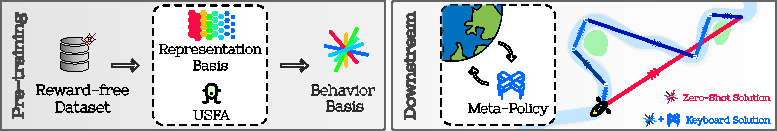
\includegraphics[width=\textwidth]{intro_horizontal.pdf}}
\caption{
Overview of the Laplacian Keyboard.
(\emph{Left}) A reward-free dataset is used to learn a representation basis and a USFA, inducing a behavior basis, which are directions in a latent space. For illustration, in this figure, we depict those as behaviours following \textit{straight-line trajectories}.
(\emph{Right}) In a downstream navigation task, an agent (the boat) executes these options to interact with the environment. A zero-shot policy picks and executes one single option, producing a potentially suboptimal trajectory (red), whereas the LK trains a meta-policy that sequentially selects and switches between options, composing a piecewise trajectory (blue) that better matches the task.
\looseness=-1}
\label{fig:lk_dumb}
\end{figure*}



% A reward-free dataset is used to learn a representation basis and an USFA, inducing a behavior basis for downstream control (illustrated here as straight-line behaviors). Given a downstream task, a meta-policy is trained to select and stitch these behaviors.
% While the zero-shot policy is restricted to a single linear combination of the basis and may be suboptimal, the Laplacian Keyboard composes multiple basis elements sequentially, producing a piecewise trajectory that more closely approximates the optimal behavior.




Representation-based methods learn features to approximate a task-relevant quantity. Proto-Value Functions \citep[PVF;][]{mahadevan2005proto}, an early RL example of this principle, employs graph Laplacian eigenvectors as a basis for value function approximation. Given a new task, the agent learns the linear weights that combine these eigenvectors to approximate the optimal value function. More recently, Forward-Backward representations \citep[FB;][]{touati2022does} learn a low-rank representation of the successor measure of a policy class, which is then used to approximate reward functions. For any new task, the agent infers the weights that best approximate the corresponding reward function for this basis. If the learned representation spans the reward function, FB produces the optimal policy with no further learning involved. This enables FB to produce \textit{zero-shot} solutions. However, this zero-shot solution is constrained by the linear span of the learned features---the policy can be suboptimal when the task lies outside this span. \looseness = -1

The second category learns a basis of behaviors \citep[or options;][]{sutton1999between} rather than features. Given a new task, these methods use generalized policy improvement \citep[GPI;][]{barreto2017successor} by evaluating each option in the basis and combining them using linear weights, guaranteeing performance at least as good as that of the best individual option, and often better. The Option Keyboard framework~\citep{barreto2019option} extends this idea by learning state-dependent weights, enabling the agent to dynamically \textit{stitch} together options across states. This allows the agent to solve a broader class of tasks than is possible with a single fixed combination of the behavior basis. However, a central limitation is that the choice of the option basis is not well defined and typically relies on manual specification of either the options or their associated reward functions. \looseness = -1


In this work, we bridge representation- and behavior-based approaches through the Laplacian Keyboard (LK), a framework that exploits their coupling for option discovery. We show that graph Laplacian eigenvectors serve dual roles: as a basis for reward approximation and as a principled, task-agnostic source of behaviors \cite{machado2023temporal}. LK combines these eigenvectors, learned from an offline, reward-free dataset, with Universal Successor Feature Approximators \citep[USFA;][]{borsauniversal} to guarantee zero-shot optimal policies for tasks whose rewards lie within the span of the learned basis.


Many downstream tasks, however, fall outside this regime. To address this limitation, LK introduces efficient adaptation via sequential composition (see Figure~\ref{fig:lk_dumb}). Rather than relying on a single linear combination of basis elements, LK decomposes complex tasks into simpler subproblems. Each USFA-induced policy becomes a reusable option in a library of task-agnostic behaviors, and a meta-policy learns to select and stitch these options efficiently. This hierarchical structure enables LK to solve tasks whose reward functions cannot be represented within the basis span. By unifying zero-shot optimality within the basis with efficient composition beyond it, LK overcomes key limitations of both representation- and behavior-based methods.


This work makes two key contributions. (1) We establish graph Laplacian eigenvectors as an effective reward basis through empirical evidence and theoretical analysis, including value-function approximation error bounds that characterize the expressivity of a finite Laplacian basis. (2) We introduce the Laplacian Keyboard, a hierarchical framework that stitches Laplacian-induced behaviors via a meta-policy, outperforming zero-shot baselines while achieving superior sample efficiency compared to standard RL agents. \looseness=-1


\section{Background}

We first formalize the problem addressed by LK and then review related approaches that tackle the same problem by learning a basis of representations or behaviors. We use calligraphic capitals for sets (e.g., $\mathscr{S}, \mathscr{A}$), capitals for random variables (e.g., $S_t, A_t$), bold capitals for matrices (e.g., $\mathbf{L}, \pp$), non-bold lowercase for functions (e.g., $\pi, r$), and bold lowercase for vectors (e.g., $\mathbf{w}, \ei$). Functions over the state or action space are often represented in vectorized form by indexing their values, denoted using bold notation (e.g., $\mathbf{r}$). \looseness=-2


\subsection{Problem Definition}

In RL, the agent-environment interaction is modeled as a Markov Decision Process (MDP) $M = (\mathscr{S}, \mathscr{A}, p, r, \gamma)$, with state space $\mathscr{S}$, action space $\mathscr{A}$, transition dynamics $p(\cdot\mid s,a)$, and discount factor $\gamma$. In this work, we define the reward $r$ as a function of the next state. Specifically, for any transition $(s, a, s')$, the state-based reward is given by $r(s') = \int_{s,a} p(s' \mid s, a)\, r(s, a, s') \, ds \, da$. The goal is to learn a policy $\pi:\mathscr{S} \to \Delta(\mathscr{A})$ that maximizes discounted expected return, expressed via the action-value function $q_\pi(s,a) = \mathbb{E}_\pi\Big[\sum_{t=0}^\infty \gamma^t r(S_{t+1}) \mid S_0=s, A_0=a \Big]$, where $S_{t+1} \sim p(\cdot\mid S_t,A_t)$.

In this work, we aim to learn a basis of behaviors that an agent can employ to output near-optimal policies for any given reward function in a sample-efficient manner. Similar to \citet{touati2022does} and \citet{agarwal2025proto}, we formulate this objective as a two-phase process, commonly referred to as \textit{Unsupervised RL}. In the pre-training phase, the agent interacts with the environment for $M$ steps to learn the basis without access to any reward function. In the subsequent downstream phase, tasks are specified through reward functions, and the agent must leverage its prior knowledge to solve these tasks within $N$ steps, where $N \ll M$. \looseness = -1


\subsection{Solution Methods}

In this section, we provide a brief overview of related unsupervised RL methods, organized by whether they use \textit{representations} or \textit{options} as the underlying basis. A more detailed review is given in Appendix~\ref{sec:extended-related-work}.


\textbf{Representation-based methods} learn a state representation $\phi:\mathscr{S} \rightarrow \mathbb{R}^d$ of dimension $d$ during pre-training, defining a representation basis to approximate downstream rewards as:
\[
r(s) \approx \mathbf{w}^\top \bp(s), \quad \forall s \in \mathscr{S}.
\]
Simultaneously, a USFA is used to train a policy $\pi(a \mid s, \mathbf{w})$ \citep{borsauniversal}. In the downstream phase, once a task is specified, a weight vector $\mathbf{w}$ is estimated from $N$ samples via simple linear regression to approximate the reward function, which parameterizes the USFA. When the reward function lies exactly within the span of $\bm{\phi}$, the USFA recovers the optimal policy, making the choice of $\bm{\phi}$ and the USFA training procedure critical (see \citet{touati2022does, borsauniversal, ollivier2025features} for further discussion). This quick adaptation using only a few samples via linear regression is referred to as \textit{zero-shot} learning by \citet{touati2022does}. \looseness=-1

Methods like Forward-Backward Representations \citep{touati2022does} and Proto Successor Measure \citep{agarwal2025proto} model $\bm{\phi}$ as a low-rank representation of the successor measure of a class of policies. These approaches have been shown to scale to large state and action spaces with minimal human prior \citep{tirinzonizero}. The primary limitation of these approaches is expressivity: the linear span of $\bm{\phi}$ must be rich enough to approximate all potential downstream rewards, often requiring a high-dimensional $d$ to cover a diverse set of complex tasks.\looseness=-1


\textbf{Option-based methods} take a complementary approach by learning a reusable option basis that can be linearly combined to solve new tasks. Most methods assume access to reward features $\phi:\mathscr{S} \rightarrow \mathbb{R}^d$, which define this basis: each option is trained to be optimal for a reward induced by these features. For downstream rewards of the form $r(s)=\mathbf{w}^\top \bm{\phi}(s)$, options can be combined via General Policy Evaluation and Improvement \citep[GPE \& GPI;][]{barreto2020fast}, yielding a policy at least as good as any individual option. We refer to \citet{borsauniversal} for details on GPE \& GPI and its connection to the USFA framework. \looseness=-1

The Option Keyboard (OK) framework \citep{barreto2019option} generalizes this approach by learning a meta-policy $\pi_{\text{OK}}$ that composes options using state-dependent weights at execution time, rather than a single fixed combination, enabling solutions to a broader class of tasks \citep{chandrasekar2025towards}. However, OK has two key limitations: (1) it relies on manually specified reward features $\bm{\phi}$, and (2) lacks a principled procedure for constructing the option basis. While \citet{alegre2025constructing} partially addresses the latter, dependence on handcrafted features remains a central limitation when such features are difficult to specify. We discuss this work further in Section~\ref{sec:exp_alegre}.



\section{The Laplacian Basis}


\begin{figure}[t]
% \begin{center}
\centerline{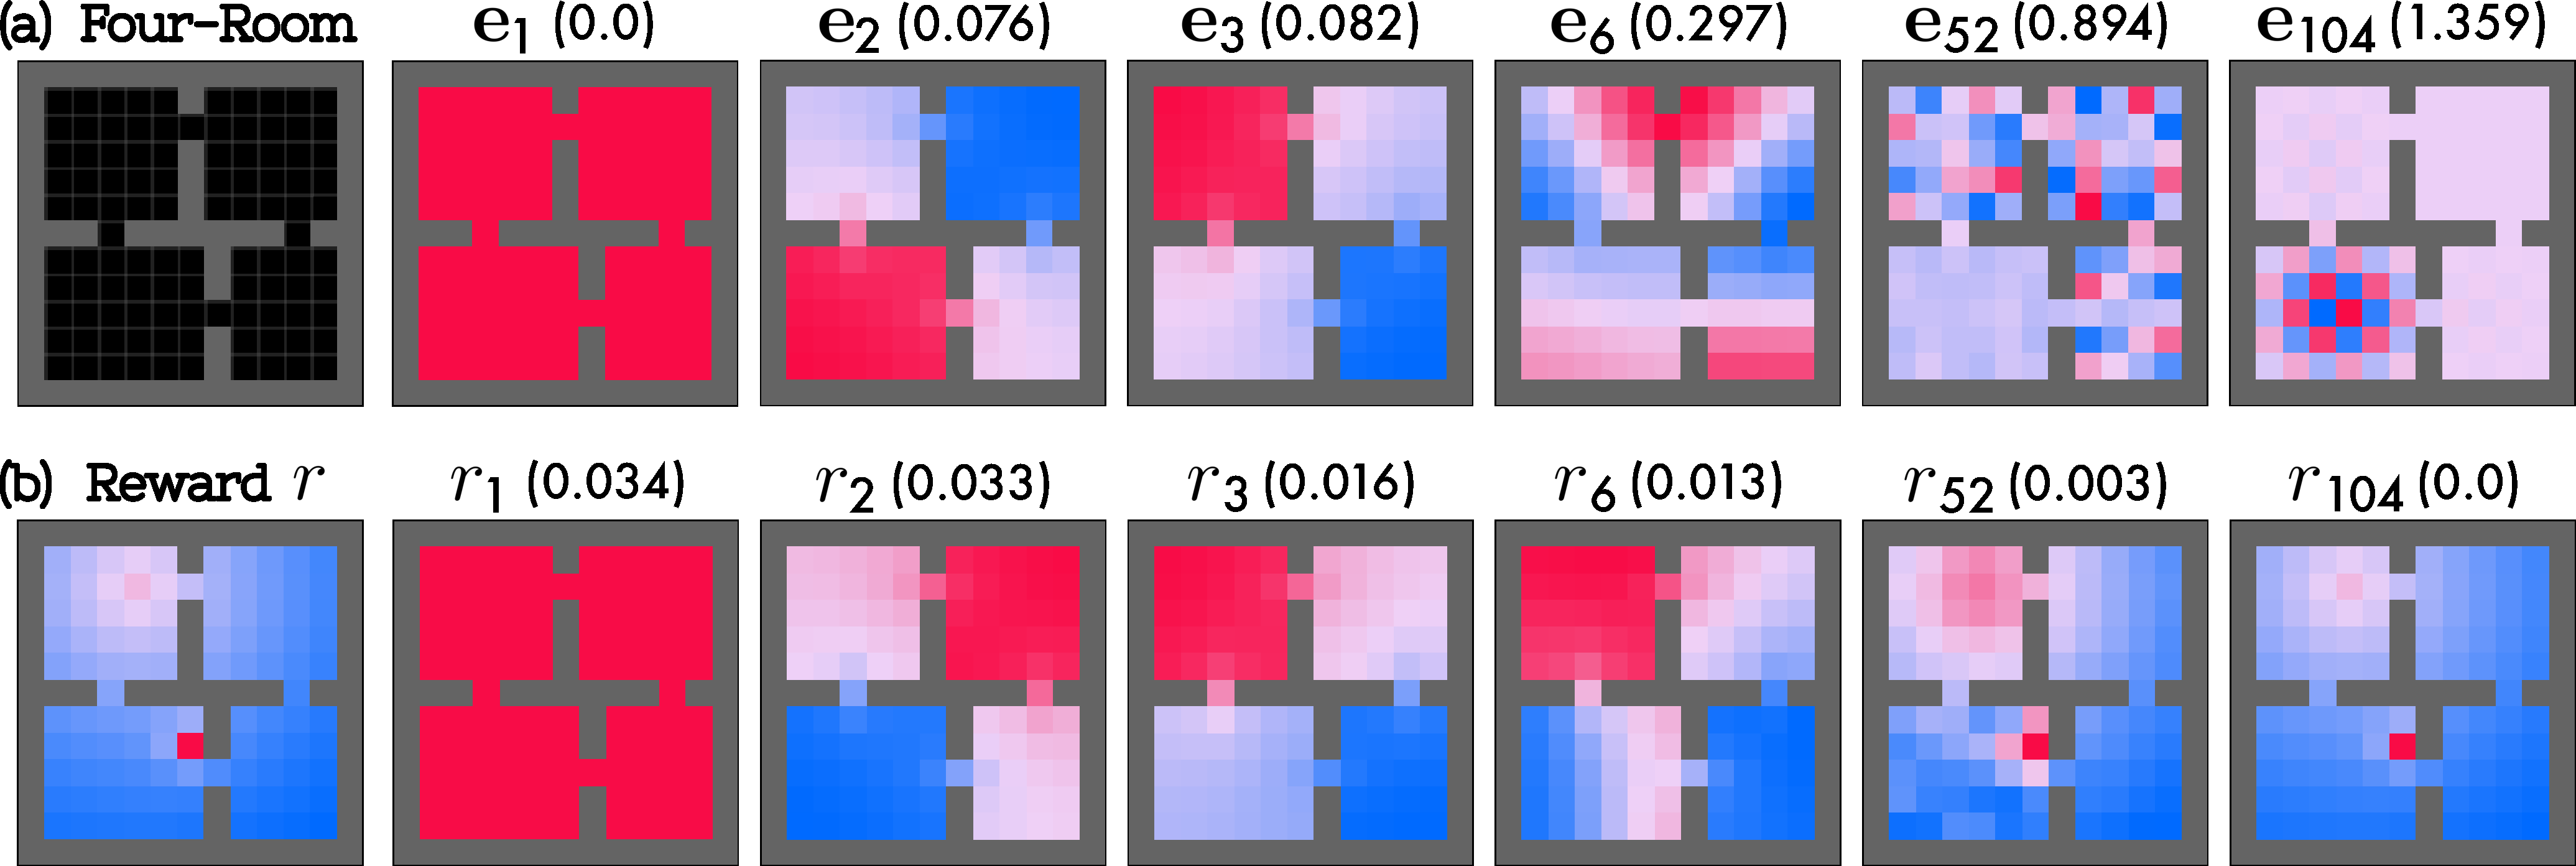
\includegraphics[width=\columnwidth]{lap_basis.pdf}}
\caption{We illustrate the Laplacian basis in the \texttt{Four-Room} environment, a toy domain introduced by \citet{sutton1999between}. The hotter (redder) the state's color, the larger the corresponding entry; color scales are normalized independently for each subplot. \textbf{(a)} Selected eigenvectors of the graph Laplacian induced by a uniform random policy, with values in parentheses indicating the eigenvector graph norm (Eqn.~\ref{eqn:grap-norm}). \textbf{(b)} A sample reward function and its reconstruction using the first $k$ eigenvectors. Values in parentheses denote the mean squared error between the original and reconstructed reward functions. Increasing the basis size improves reconstruction accuracy.}
\label{fig:eigvecs}
\end{figure}



This section motivates the use of graph Laplacian eigenvectors as a basis for approximating reward functions.

We restrict ourselves to MDPs in which the induced Markov chain under any policy of interest is reversible \citep{levin2017markov}. 
% In informal terms, whenever a transition $(s,a) \to (s',a')$ can occur, the reverse transition $(s',a') \to (s,a)$ is also admissible. 
Any such MDP can be modeled as an undirected graph, with states as vertices and transitions as edges.\footnote{See Appendix \ref{apdx:gft_bg} for an in-depth background.} 
In the discrete case, the graph Laplacian is defined as $\mat{L} \, \dot{=} \, \mat{I} - \pp$, where $\pp(s, s') = \sum_{a \in \mathscr{A}} \pi(s, a) p(s'|s, a)$ denotes the probability of going from state $s$ to $s'$ under policy $\pi$. Let $\ei_i$ denote the $i$-th eigenvector of $\mat{L}$, with eigenvector ordering defined by their corresponding eigenvalue. These eigenvectors encode the structural properties of the state space in a natural order: eigenvectors associated with smaller eigenvalues are smoother, ranging from the constant vector $\ei_1$ to progressively more oscillatory patterns as the eigenvalue increases (see Figure~\ref{fig:eigvecs}a).



To formalize this notion of smoothness, we rely on the \textit{graph norm} \citep{zhu2012approximating}; for any function $f: \mathscr{S} \to \mathbb{R}$ defined over the state space:
\begin{equation}
    \|f\|_G \, \dot{=} \, \left[ \frac{1}{2}  \sum_{(i,j) \in \mathscr{S} \times \mathscr{S}} \pp(i, j) (f(i) - f(j))^2\right]^{\frac{1}{2}}.    
    \label{eqn:grap-norm}
\end{equation}

The graph norm penalizes local variations weighted by the transition probabilities, smaller values indicating that the signals vary smoothly across connected states (see Figure~\textcolor{neelam}{\ref{fig:eigvecs}a}). \looseness = -1


The Laplacian representation is the mapping $\phi: \mathscr{S} \rightarrow \mathbb{R}^k$ ($0 < k \le |\mathscr{S}|$), defined by $\bp(s) = [\ei_1[s], \ei_2[s], \dots, \ei_k[s]]$, where $\ei_i[s]$ denotes the $s$-th entry of eigenvector $\ei_i$. The eigenvectors of $\mat{L}$ form an orthonormal basis spanning the entire state-space function class. Stacking the Laplacian representations of all states yields the \textit{Laplacian basis} $\mathbf{\Phi} \in \mathbb{R}^{|\mathscr{S}|\times k}$. Using the complete basis ($k = |\mathscr{S}|$), any reward function ${r}: \mathscr{S} \to \mathbb{R}$ admits an exact decomposition: $\mathbf{r}_k \, \dot{=} \, \mathbf{\Phi} \, (\mathbf{\Phi}^\top \mathbf{r})$ (the least-squares solution). However, for environments with large state spaces, computing and storing the full basis is infeasible.


This constraint requires restricting the representation to the first $k \ll |\mathscr{S}|$ eigenvectors, imposing an inductive bias. These eigenvectors, corresponding to the smallest eigenvalues, capture the lowest-frequency components of functions defined over the state space. As a result, any reward function with significant high-frequency structure lies outside the span of this truncated basis and cannot be reconstructed exactly (Figure~\textcolor{neelam}{\ref{fig:eigvecs}b}). This mismatch propagates to the prediction problem: the optimal value function computed from the approximated reward need not coincide with true optimal value function. Theorem \ref{theorem:the-one-main-paper} bounds this mismatch.

\begin{theorem}[\ValueApproxName]
Let $r: \mathscr{S} \to \mathbb{R}$ be a reward function with bounded variation\footnote{A formal definition of \textit{bounded variation} is provided in Eqn.~\ref{eqn:bounded_variation} in Appendix~\ref{sec:app_background}. Intuitively, it requires the reward function to vary smoothly over the state space.} and $\mathbf{r}_k$ its reconstruction using the first $k$ eigenvectors. Let $\mathbf{v}^*$ and $\mathbf{v}^*_k$ be their corresponding optimal value functions. Then,
\begin{equation}
    \|\mathbf{v}^* - \mathbf{v}^*_k\|_\infty \le \frac{\|r\|_G}{(1-\gamma)\sqrt{\lambda_k}},
\end{equation}
where $\lambda_k$ is the $k$-th eigenvalue.
\label{theorem:the-one-main-paper}
\end{theorem}

The proof is provided in Appendix \ref{sec:proof}. It proceeds by first establishing an upper bound on the reconstruction error of the reward function when using the first $k$ eigenvectors of the graph Laplacian, then using the Bellman contraction property to show that this error amplifies by no more than $(1-\gamma)^{-1}$, yielding the stated bound on the value function. 

The bound reveals two key factors influencing approximation error. 
(1) Reward functions that vary smoothly over the state space, reflected by a smaller value of $\|r\|_G$, incur smaller errors.
(2) Increasing the basis size improves approximation quality: for the normalized Laplacian, eigenvalues satisfy $\lambda_k \in [0,2]$, and larger $k$ corresponds to incorporating higher-frequency components, tightening the bound.
Together, they characterize how signal smoothness and basis dimensionality jointly determines the correctness of the induced value function. \looseness=-1



\begin{figure}[t]
\centerline{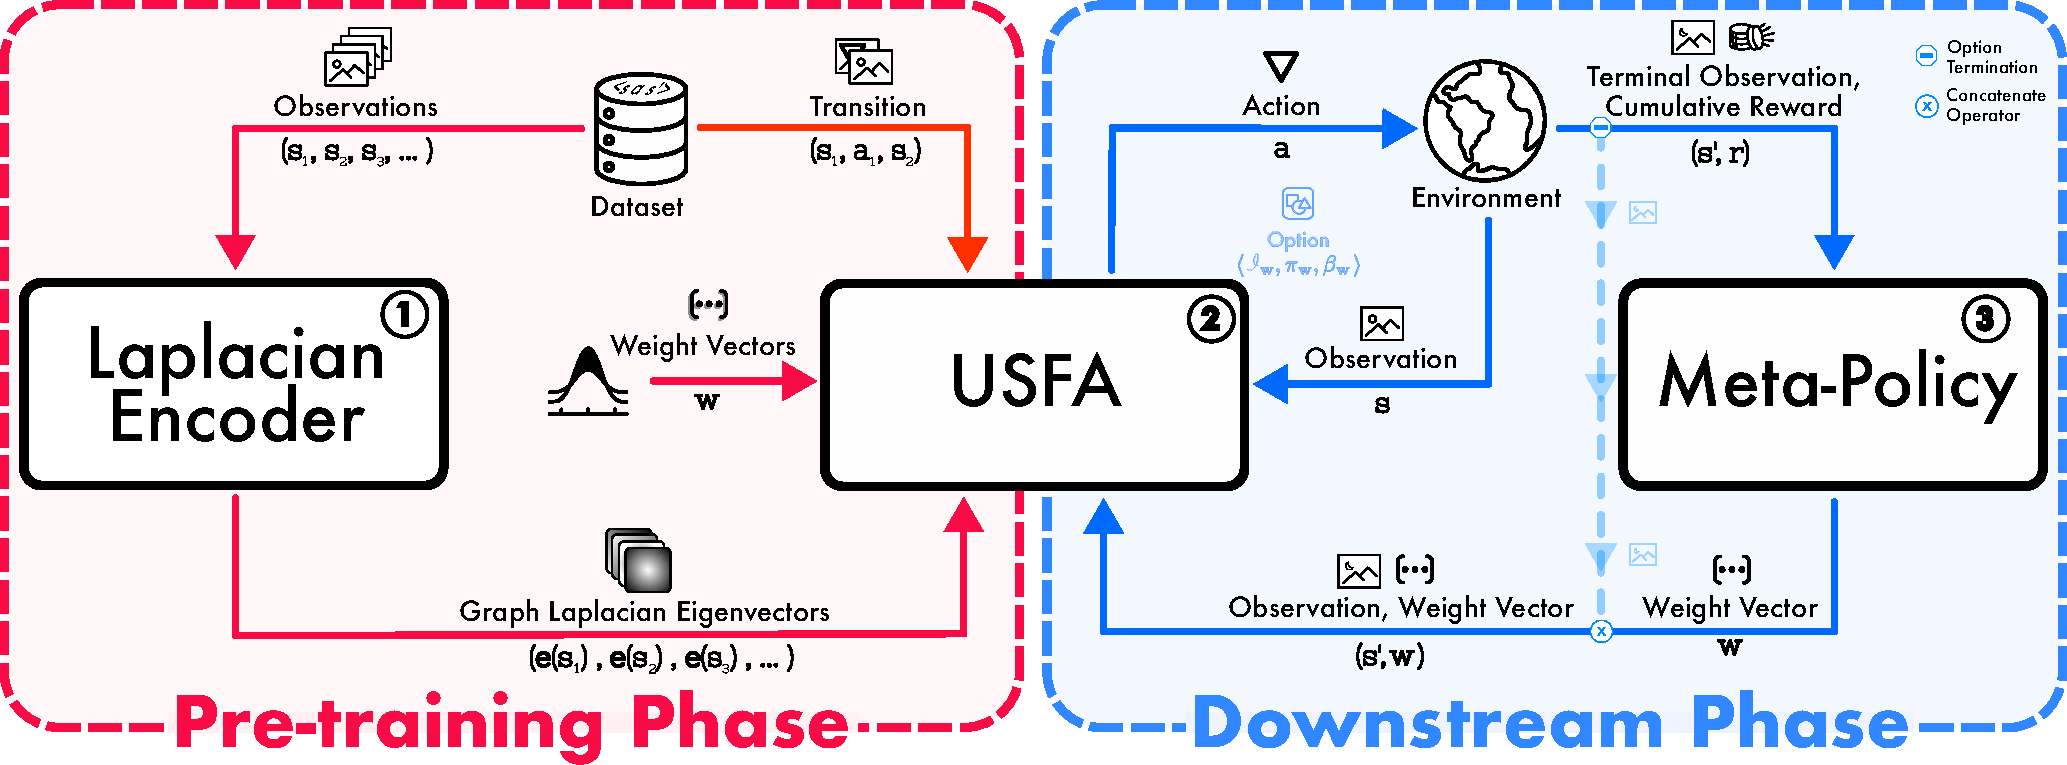
\includegraphics[width=\columnwidth]{lk_detail.pdf}}
\caption{The Laplacian Keyboard Framework. During pre-training, the agent first learns graph Laplacian eigenvectors through the Laplacian Encoder \circled{1}, then uses these as state representations to learn a continuous library of options via a USFA \circled{2}. In the downstream phase, a meta-policy \circled{3} learns to stitch these base policies, enabling rapid and sample-efficient adaptation to new tasks. Numbers indicate the learning sequence of each module.}
\label{fig:lk_detail}
\end{figure}

\section{The Laplacian Keyboard}

Having established the Laplacian representation as an effective basis, we introduce the Laplacian Keyboard (Figure~\ref{fig:lk_detail}) and describe its construction and use for control.

\subsection{Pre-training Phase}

We assume access to a reward-free dataset, $\mathscr{D}$, that induces a transition kernel, $\pp$, and its graph Laplacian, $\mathbf{L}$. We approximate the first $k$ eigenvectors of $\mathbf{L}$ using the Augmented Laplacian Objective \citep[ALLO;][]{gomezproper}:

\vspace{-15pt}

\begin{flalign*}
& \max_{\boldsymbol{\beta}} \min_{\mathbf{u} \in \mathbb{R}^{k|\mathscr{S}|}}
  \underbrace{\sum_{i=1}^k \langle \mathbf{u}_i, \mathbf{L}\mathbf{u}_i \rangle}_{\text{smoothness term}}
  \;+\; && \\
& \underbrace{
    \sum_{j=1}^k \sum_{k=1}^j 
    \Big[
      \beta_{jk}\big( \langle \mathbf{u}_j, \llbracket \mathbf{u}_k \rrbracket \rangle - \delta_{jk} \big)
      + b\,\big( \langle \mathbf{u}_j, \llbracket \mathbf{u}_k \rrbracket \rangle - \delta_{jk} \big)^2
    \Big]
  }_{\text{orthogonality-enforcing terms}}
&&
\end{flalign*}

\vspace{-5pt}


where $\mathbf{u}_i \in \mathbb{R}^{|\mathscr{S}|}$ denotes the learned approximation to the $i$-th Laplacian eigenvector $\ei_i$, $\boldsymbol{\beta} = \{\beta_{jk}\}$ are Lagrange multipliers enforcing orthonormality, $\delta_{jk}$ is the Kronecker delta, and $b > 0$ is a hyper-parameter. The notation $\llbracket \mathbf{u}_k \rrbracket$ denotes a stop-gradient operation. For notational simplicity, we henceforth use $\ei_i$ to denote the learned eigenvectors $\mathbf{u}_i$ obtained from this optimization.

% We train a USFA, which maps reward functions to value functions through successor features \citep[SFs][]{barreto2017successor}, a generalization of successor representations \citep{dayan1993improving}. Using the Laplacian basis $\bp(s) \in \mathbb{R}^k$, any weight vector $\mathbf{w}$ defines a reward function $r_{\mathbf{w}}(s) = \mathbf{w}^\top \bp(s)$. The USFA is conditioned on $\mathbf{w}$ and comprises a policy $\pi_{\mathbf{w}}$ and a SF estimator, $\bm{\psi}_{\mathbf{w}}$.

% The SFs encode the expected discounted accumulation of Laplacian features under the conditioned policy:
% \begin{equation}
%     \bm{\psi}(s,a,\mathbf{w}) =
%     \mathbb{E}_{\pi_{\mathbf{w}}}\!\left[
%     \sum_{t=0}^{\infty} \gamma^t \bp(S_{t+1})
%     \,\middle|\,
%     S_0 = s,\, A_0 = a
%     \right].
% \end{equation}
% Training is performed off-policy using transitions $(s,a,s')$ drawn from a dataset $\mathscr{D}$ with empirical dynamics $p_{\mathscr{D}}(\cdot \mid s,a)$. During learning, weight vectors $\mathbf{w}$ are sampled and used to condition both the policy and the SF estimator. The SFs are learned by enforcing Bellman consistency,
% \begin{equation}
%     \bm{\psi}(s,a,\mathbf{w})
%     =
%     \bp(s') + \gamma
%     \mathbb{E}_{a' \sim \pi_{\mathbf{w}}(\cdot \mid s')}
%     \bm{\psi}(s',a',\mathbf{w}),
% \end{equation}
% where $s' \sim p_{\mathscr{D}}(\cdot \mid s,a)$. Under exact representation, the USFA recovers optimal policies for all reward functions in the span of the $k$ Laplacian eigenvectors, with the corresponding action-value function given by
% $q^*_{\mathbf{w}}(s,a) = \mathbf{w}^\top \bm{\psi}(s,a,\mathbf{w})$
% \citep{borsauniversal}. In continuous action spaces, $\pi_{\mathbf{w}}$ is optimized using policy gradients with this value estimate, while in discrete action spaces actions are selected greedily as $\arg\max_a \mathbf{w}^\top \bm{\psi}(s,a,\mathbf{w})$.


We use the Laplacian representation $\bp(s) \in \mathbb{R}^k$ to parameterize a family of reward functions of the form
$r_{\mathbf{w}}(s) = \mathbf{w}^\top \bp(s)$.
To model policies and value functions for this reward family, we train a Universal Successor Feature Approximator (USFA) \citep{barreto2017successor}, which generalizes successor representations \citep{dayan1993improving} by conditioning on the reward parameter $\mathbf{w}$. The USFA consists of a policy $\pi_{\mathbf{w}}$ and a corresponding successor feature estimator $\bm{\psi}_{\mathbf{w}}$.

The successor features encode the expected discounted accumulation of Laplacian features under the conditioned policy:
\begin{equation}
    \bm{\psi}(s,a,\mathbf{w}) =
    \mathbb{E}_{\pi_{\mathbf{w}}}\!\left[
    \sum_{t=0}^{\infty} \gamma^t \bp(S_{t+1})
    \,\middle|\,
    S_0 = s,\, A_0 = a
    \right].
\end{equation}
Training is performed off-policy using transitions $(s,a,s')$ sampled from a dataset $\mathscr{D}$ with empirical dynamics $p_{\mathscr{D}}(\cdot \mid s,a)$. During training, weight vectors $\mathbf{w}$ are sampled and used to jointly condition both the policy and the successor feature estimator. The successor features are learned by enforcing Bellman consistency,
\begin{equation}
    \bm{\psi}(s,a,\mathbf{w})
    =
    \bp(s') + \gamma
    \mathbb{E}_{a' \sim \pi_{\mathbf{w}}(\cdot \mid s')}
    \bm{\psi}(s',a',\mathbf{w}),
\end{equation}
where $s' \sim p_{\mathscr{D}}(\cdot \mid s,a)$. Under exact representation, the USFA recovers optimal policies for all reward functions lying in the span of the $k$ Laplacian eigenvectors, with the optimal action-value function given by
$q^*_{\mathbf{w}}(s,a) = \mathbf{w}^\top \bm{\psi}(s,a,\mathbf{w})$.
In continuous action spaces, $\pi_{\mathbf{w}}$ is optimized using policy gradients with this value estimate, while in discrete action spaces actions are selected greedily via
$\arg\max_a \mathbf{w}^\top \bm{\psi}(s,a,\mathbf{w})$
\citep{borsauniversal}.


During training, following \citet{touati2022does}, weight vectors $\mathbf{w}$ are sampled from a broad distribution to promote wide coverage of the reward-function space. For any reward function in the linear span of the eigenvectors, the USFA can output the optimal policy. For reward functions outside this span, we have provided a bound for the sub-optimality of the resulting policies in Theorem~\ref{theorem:the-one-main-paper}. The next section describes how LK goes beyond the linear span to address a larger family of reward functions. \looseness = -1


\subsection{Downstream Phase}
\label{sec:downstream}

In the downstream phase, a meta-policy, $\pi_{\text{LK}}: \mathscr{S} \to \mathbb{R}^k$, is trained to sequence options for solving arbitrary tasks. This meta-policy generates weight vectors $\mathbf{w} \in \mathbb{R}^k$ that parameterize the USFA, which in turn produces and executes options. The hierarchical control mechanism operates as follows: $\pi_{\text{LK}}$ outputs a weight vector $\mathbf{w}$ that parameterizes the USFA to instantiate an option; this option executes for a predetermined horizon $t_{\text{term}}$ or until its termination condition is satisfied; control then returns to $\pi_{\text{LK}}$, which selects a new weight vector based on the new state. This process continues iteratively until the task is solved. \looseness = -1


When the downstream reward function $r$ lies within the span of the learned eigenvectors $\ei$, the meta-policy recovers the optimal weight vector $\mathbf{w}$ satisfying $r(s)=\mathbf{w}^\top\bp(s)$, achieving zero-shot transfer as in other representation-based methods. For out-of-span rewards, the meta-policy approximates the optimal policy by sequencing multiple options~\citep{alegre2025constructing}, stitching locally optimal behaviors induced by different weight vectors into a near-optimal global policy (see Figure~\ref{fig:lk_example}). This compositional structure enables LK to address reward functions beyond the linear span of the learned features.



\begin{figure}[t]
\centerline{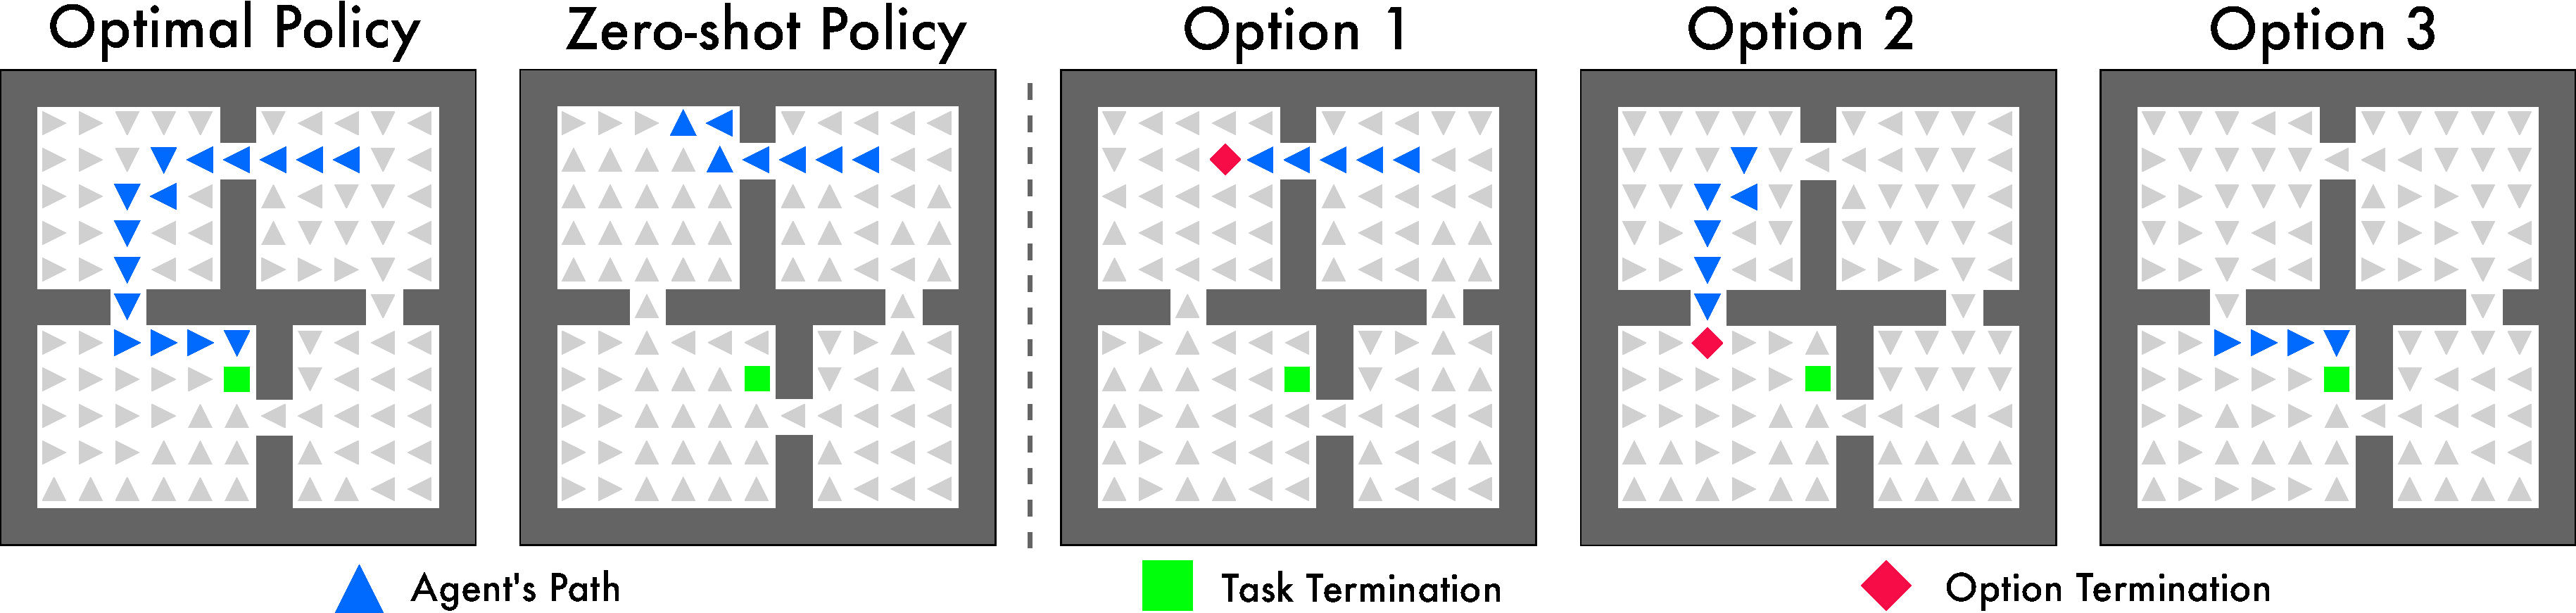
\includegraphics[width=\columnwidth]{LK_optimal_4rooms.pdf}}
\caption{%This example shows how 
The LK stitches behaviors from the learned basis to approximate the optimal policy when the reward function lies outside the span of the eigenvectors. We use the same reward function $r$ from Figure~\ref{fig:eigvecs}. The \textit{first} panel contains the optimal policy of the original reward function to reach the goal state. The \textit{second} panel displays the optimal policy of the reconstructed reward function with $k=6$ eigenvectors (${r}_6$). This policy fails to reach the goal state. The \textit{last three} panels show how LK stitches three individual options, each terminated after a fixed horizon $t_{\text{term}} = 6$.
Together, these options form a near-optimal policy that closely replicates the true optimal behavior through a hierarchical control loop. \looseness=-1}
\label{fig:lk_example}
\vspace{-15pt}
\end{figure}


When compared to prior option-based methods, LK does not rely on manually specified reward features or predefined training tasks to form the behavior basis. Instead, it is learned directly from the offline dataset. Consequently, the basis scales with the coverage of the dataset and the chosen value of $k$. In addition, we do not constrain the basis to a finite set of options; the USFA formulation provides a continuous library of option policies.


Finally, we expect LK to achieve better sample efficiency than flat agents, i.e., agents that act directly in the primitive action space, for two reasons.~(1) By learning over options rather than primitive actions, LK propagates value information across multiple timesteps, which can accelerate credit assignment \citep{sutton1999between}. (2) Exploration in this structured space corresponds to exploring over coherent, temporally-extended behaviors~\citep{machado2017laplacian,machado2023temporal,jinnai2019discovering}, which can reduce variance and enable faster downstream learning. However, unlike previous approaches, here the action space of $\pi_{\text{LK}}$ is the continuous space of weight vectors $\mathbf{w}$ that parameterize options. This induces a smooth control space in which small changes in the policy output lead to similar behaviors, instead of having small parameter changes producing qualitatively different action sequences.  \looseness=-1


\section{Laplacian Behavior Basis}

Here we visualize the behaviors induced by the graph Laplacian eigenvectors in the DeepMind Control suite \citep[DMC;][]{tassa2018deepmind}. We consider three domains: \textsc{Cheetah}, \textsc{Quadruped}, and \textsc{Walker}---corresponding to agents with distinct morphologies and control dynamics. Observations consist of joint positions and velocities; additional environment details are provided in Appendix~\ref{sec:environments}. We use the offline dataset from \citet{yarats2022exorl}, which contains trajectories collected under diverse exploration strategies.

Figure~\ref{fig:behaviors} illustrates the behaviors induced by the first Laplacian eigenvector across the three domains, corresponding to the negative ($\mathbf{w}_{-\mathbf{e}{_1}}$) and positive ($\mathbf{w}_{+\mathbf{e}{_1}}$) directions of that eigenvector. Although the specific behaviors differ across environments, the two directions consistently induce opposing outcomes. In \textsc{Cheetah}, the negative direction produces forward hopping, while the positive direction results in an inverted posture. In \textsc{Quadruped}, the negative direction yields an inverted stance, whereas the positive direction induces an upright posture. In \textsc{Walker}, the negative direction leads to a backward headstand, while the positive direction produces a forward headstand. We observe similar oppositional structure for other eigenvector directions and across multiple runs. These behaviors emerge without hand-crafted priors, providing a scalable mechanism for learning a behavioral basis without explicitly enumerating skills.

\begin{figure}[t]
\centerline{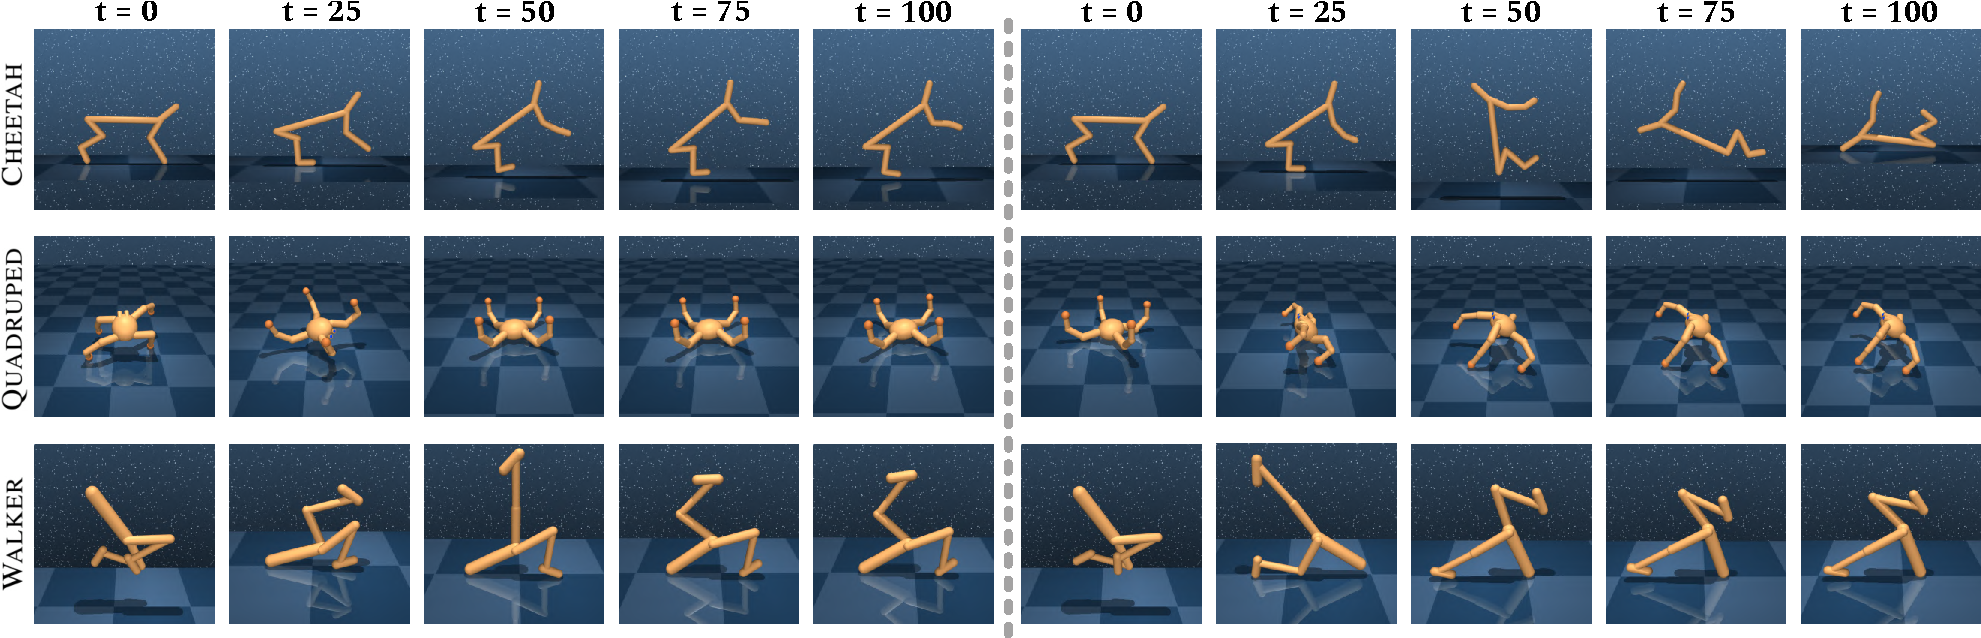
\includegraphics[width=\columnwidth]{behaviors_compressed.pdf}}
\caption{Instances from the Laplacian behavior basis. The left panel shows the behavior corresponding to $\mathbf{w}_{-\mathbf{e}{_1}}=[-1, 0, 0, \dots]$, while the right panel shows the behavior corresponding to $\mathbf{w}_{+\mathbf{e}{_1}}=[+1, 0, 0, \dots]$. \looseness=-1}
\label{fig:behaviors}
\vspace{-10pt}
\end{figure}



\section{Empirical Validation on DMC}

Building on the preceding analysis, we empirically examine two key properties of the Laplacian behavior basis and its use within LK.
(1) Laplacian eigenvectors provide a task-agnostic representational basis that supports zero-shot RL.
(2) The hierarchical structure of LK enables sample-efficient learning that extends beyond what can be achieved through linear combinations of the basis alone.


\paragraph{Environment:} We consider four tasks in each of the DMC domains: \textsc{Cheetah} (\texttt{Run, Run Backwards, Walk, Walk Backwards}), \textsc{Quadruped} (\texttt{Jump, Run, Stand, Walk}), and \textsc{Walker} (\texttt{Flip, Run, Stand, Walk}). Backward variants are denoted with a \texttt{-B} suffix (e.g., \texttt{Run-B}). Each domain includes offline datasets from three exploration policies: \texttt{APS}, \texttt{Proto}, and \texttt{RND} \cite{yarats2022exorl}. The diversity of domains, tasks, and data-collection strategies makes DMC a suitable benchmark for evaluating the representational and learning properties of LK.

\paragraph{Implementation:} For each domain--dataset pair and a given basis size $k$, we train a Laplacian encoder and a corresponding USFA policy, resulting in 9 pre-trained agents that are used for zero-shot evaluation. Using these pre-trained components, we then train a meta-policy for each downstream task, yielding a total of 36 meta-policies (9 domain--dataset pairs $\times$ 4 tasks). We repeat this procedure for basis sizes $k \in \{1, 2, 3, 5, 10, 20, 50\}$. Both the USFA and the meta-policies are trained using TD3 \citep{fujimoto2018addressing}. Zero-shot performance is evaluated using 10K labeled samples, while each meta-policy is trained for 200K environment interactions. To contextualize task difficulty, we additionally train a flat TD3 agent for 2M interactions. Both the meta-policy and the flat baseline are evaluated every 10K interactions over 10 episodes, and all results are averaged over 30 independent runs.


\begin{table}[t]
\centering
\caption{Comparison of zero-shot performance between FB, LK ($k=50$), and a flat TD3. Reported values are the mean $\pm$ standard error, averaged over 30 independent runs for each of the three datasets (90 runs total per entry).}
\setlength{\tabcolsep}{6pt}
\renewcommand{\arraystretch}{1.3}
\footnotesize
\label{tab:zero-shot-comp}
\begin{tabular}{lrrr}
\toprule
\textbf{Task} & \textbf{FB} & \textbf{LK} & \textbf{Flat TD3} \\
\midrule

\rowcolor{gray!15}
\textsc{Cheetah} \textit{(avg)} & 552 & 450 & 786 \\
\hspace{.5em} \texttt{Run} & 248 ${\scriptstyle \pm 7}$ & 196 ${\scriptstyle \pm 9}$ & 714 ${\scriptstyle \pm 13}$ \\
\hspace{.5em} \texttt{Run-B} & 229 ${\scriptstyle \pm 4}$ & 188 ${\scriptstyle \pm 6}$ & 471 ${\scriptstyle \pm 15}$ \\
\hspace{.5em} \texttt{Walk} & 819 ${\scriptstyle \pm 15}$ & 709 ${\scriptstyle \pm 22}$ & 980 ${\scriptstyle \pm 2}$ \\
\hspace{.5em} \texttt{Walk-B} & 912 ${\scriptstyle \pm 10}$ & 706 ${\scriptstyle \pm 14}$ & 981 ${\scriptstyle \pm 1}$ \\
\addlinespace
\rowcolor{gray!15}
\textsc{Quadruped} \textit{(avg)} & 470 & 509 & 592 \\
\hspace{.5em} \texttt{Jump} & 483 ${\scriptstyle \pm 7}$ & 554 ${\scriptstyle \pm 10}$ & 625 ${\scriptstyle \pm 38}$ \\
\hspace{.5em} \texttt{Run} & 317 ${\scriptstyle \pm 6}$ & 366 ${\scriptstyle \pm 5}$ & 456 ${\scriptstyle \pm 31}$ \\
\hspace{.5em} \texttt{Stand} & 617 ${\scriptstyle \pm 12}$ & 705 ${\scriptstyle \pm 14}$ & 708 ${\scriptstyle \pm 35}$ \\
\hspace{.5em} \texttt{Walk} & 461 ${\scriptstyle \pm 9}$ & 410 ${\scriptstyle \pm 11}$ & 578 ${\scriptstyle \pm 48}$ \\
\addlinespace
\rowcolor{gray!15}
\textsc{Walker} \textit{(avg)} & 584 & 582 & 780 \\
\hspace{.5em} \texttt{Flip} & 412 ${\scriptstyle \pm 13}$ & 507 ${\scriptstyle \pm 15}$ & 667 ${\scriptstyle \pm 7}$ \\
\hspace{.5em} \texttt{Run} & 356 ${\scriptstyle \pm 7}$ & 294 ${\scriptstyle \pm 9}$ & 571 ${\scriptstyle \pm 15}$ \\
\hspace{.5em} \texttt{Stand} & 754 ${\scriptstyle \pm 13}$ & 635 ${\scriptstyle \pm 23}$ & 977 ${\scriptstyle \pm 2}$ \\
\hspace{.5em} \texttt{Walk} & 816 ${\scriptstyle \pm 8}$ & 890 ${\scriptstyle \pm 11}$ & 905 ${\scriptstyle \pm 17}$ \\
\addlinespace

\bottomrule
\end{tabular}
\vspace{-5pt}
\end{table}


\subsection{Generality of the Laplacian Basis}

We first assess whether the Laplacian basis can linearly approximate arbitrary reward functions through zero-shot evaluation. For comparison, we use Forward-Backward representations (FB), which has shown great promise \cite{touati2022does, tirinzonizero} with theoretical guarantees \cite{blier2021learning}. Accordingly, we expect LK's zero-shot performance to be atleast comparable with FB and competitive with a strong oracle up to a constant factor.

Table~\ref{tab:zero-shot-comp} presents zero-shot performance for a basis size of $k=50$, with results averaged across the three datasets unless noted otherwise. We focus on $k=50$ here, with additional results provided in Appendix~\ref{sec:generality-appx}, as this basis size was used in \citet{touati2022does}, where performance was reported to plateau for larger values of $k$. We use a task-specific flat TD3 agent as an oracle baseline. 
LK achieves strong zero-shot performance comparable to FB; a sign test finds no significant difference between the two methods, indicating that the Laplacian basis matches the expressiveness of this established alternative.
Relative to the oracle, LK attains at least 75\% of oracle return on 8 of 12 tasks, indicating effective approximation of a broad class of reward functions. This behavior is particularly pronounced in the \textsc{Quadruped} domain, where LK achieves near-oracle performance across all tasks. For clarity, we report only LK's zero-shot results in subsequent sections to facilitate direct comparison with downstream performance. \looseness=-1


Figure~\ref{fig:lk-lineplot-main} further presents LK’s zero-shot performance as a function of the basis size. In \textsc{Cheetah} and \textsc{Walker}, performance generally improves with increasing basis size. For most tasks, improvements are gradual, while a small number exhibit sharp gains, suggesting that those additional basis components typically contribute incrementally, with occasional dominant directions.

In contrast, \textsc{Quadruped} achieves its strongest performance with the smallest basis ($k=1$), with performance degrading slightly as the basis size increases. This suggests that the leading eigenvector captures most of the task-relevant structure, while higher-order components provide limited additional benefit. We observe that the first eigenvector induces behaviors that regulate torso elevation, central to the reward functions of all four tasks, and discuss this effect in detail in Appendix~\ref{sec:quadruped}.


\begin{figure}[t]
\centerline{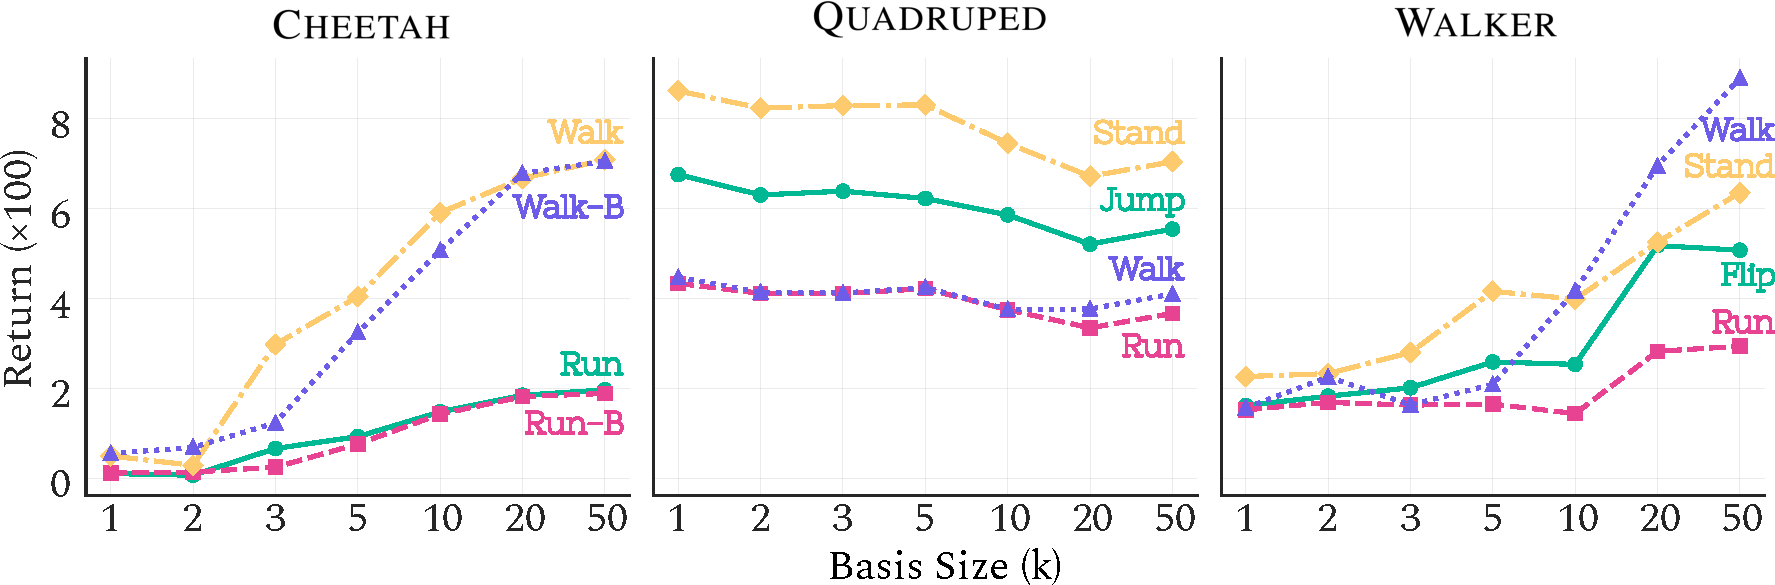
\includegraphics[width=\columnwidth]{lk-lineplot-main.pdf}}
\caption{Zero-shot performance of LK for varying basis sizes, averaged over 30 independent runs for each of the three datasets (90 runs total per curve).}
\label{fig:lk-lineplot-main}
\vspace{-15pt}
\end{figure}


\subsection{Hierarchical Composition}

We next examine the benefits of LK’s hierarchical structure. Specifically, we show that hierarchy (1) enables LK to improve upon zero-shot solutions with minimal additional interaction and (2) improves sample efficiency relative to flat agents. These experiments are informative not because the basis is rich, but because it is deliberately constrained ($k \in \{1,2,3,5,10\}$), serving as a proxy for settings in which even larger bases may be insufficient.

Table~\ref{tab:perc_imp_fb_lk} reports the percentage improvement of LK after 200K environment interactions relative to its zero-shot performance. In \textsc{Cheetah} and \textsc{Walker}, LK improves over the zero-shot solution on most tasks and across most basis sizes. The improvements are largest when the behavioral basis is small, highlighting the regime in which hierarchical composition is most effective. When $k=1$, the USFA can represent only two options, corresponding to the positive and negative directions of the eigenvector, since no linear combinations are possible and scaling the weight vector has no effect. Despite this severe restriction, the meta-policy’s ability to switch between these two options yields improvements exceeding 100\% on several tasks. This illustrates a key property of LK: even highly constrained bases can be effective when coupled with hierarchical control. As $k$ increases, the magnitude of improvement generally decreases but remains largely positive, indicating that the benefits of composition are strongest when tasks require non-linear reuse of a limited set of basis behaviors. \looseness=-1


\begin{table}
\centering
\caption{Relative percentage improvement of LK over its zero-shot baseline for varying basis sizes, estimated  from 30 independent runs for each of the three datasets (90 runs total per entry).}
\label{tab:perc_imp_fb_lk}

\setlength{\tabcolsep}{1.5pt}
\scriptsize

\begin{tabular}{ 
  l
  S[table-format=4.1]
  S[table-format=4.1]
  S[table-format=4.1]
  S[table-format=4.1]
  S[table-format=4.1]
  S[table-format=3.1]
  S[table-format=3.1]
}
\toprule
 & \multicolumn{7}{c}{\textbf{Improvement (\%) for Basis Size $k$}} \\
\cmidrule(lr){2-8}
\textbf{Task} & 1 & 2 & 3 & 5 & 10 & 20 & 50 \\
\midrule

\rowcolor{gray!15} \domainavg{cheetah}  & 1296 & 2553 & 288 & 97 & 51 & 17 & 10 \\
\hspace{.5em} \texttt{Run} & 1081 & 4608 & 176 & 61 & 58 & 44 & 34 \\
\hspace{.5em} \texttt{Run-B} & 1678 & 1241 & 508 & 154 & 64 & -3 & 1 \\
\hspace{.5em} \texttt{Walk} & 808 & 3532 & 125 & 41 & 29 & 21 & 12 \\
\hspace{.5em} \texttt{Walk-B} & 1619 & 829 & 345 & 133 & 53 & 5 & -6 \\
\addlinespace
\rowcolor{gray!15} \domainavg{quadruped}  & -3 & -12 & -11 & -17 & -14 & -2 & -12 \\
\hspace{.5em} \texttt{Jump} & -3 & -13 & -13 & -19 & -26 & -7 & -13 \\
\hspace{.5em} \texttt{Run} & -3 & -11 & -13 & -21 & -15 & -2 & -17 \\
\hspace{.5em} \texttt{Stand} & 1 & -16 & -14 & -20 & -16 & -7 & -13 \\
\hspace{.5em} \texttt{Walk} & -6 & -7 & -5 & -10 & -1 & 7 & -4 \\
\addlinespace
\rowcolor{gray!15} \domainavg{walker}  & 112 & 107 & 115 & 132 & 159 & 62 & 35 \\
\hspace{.5em} \texttt{Flip} & 106 & 99 & 104 & 115 & 189 & 53 & 46 \\
\hspace{.5em} \texttt{Run} & 55 & 52 & 34 & 80 & 185 & 62 & 44 \\
\hspace{.5em} \texttt{Stand} & 118 & 145 & 119 & 79 & 136 & 97 & 49 \\
\hspace{.5em} \texttt{Walk} & 170 & 132 & 204 & 253 & 126 & 37 & 2 \\
\addlinespace


\bottomrule
\end{tabular}
\vspace{-15pt}
\end{table}


In contrast, \textsc{Quadruped} exhibits the opposite trend. LK rarely improves over its zero-shot solution across tasks and basis sizes. Consistent with observations from the previous section, tasks in this domain appear to be well approximated by the leading eigenvector. If the zero-shot weight vector is already near-optimal, hierarchical learning reduces to identifying a single weight vector in $\mathbb{R}^k$, which we hypothesize to be a challenging optimization problem. Nevertheless, LK can be constructed to choose between the zero-shot solution and hierarchical composition, guaranteeing performance no worse than the best of the two. \looseness=-1


\begin{figure*}[t]
\centerline{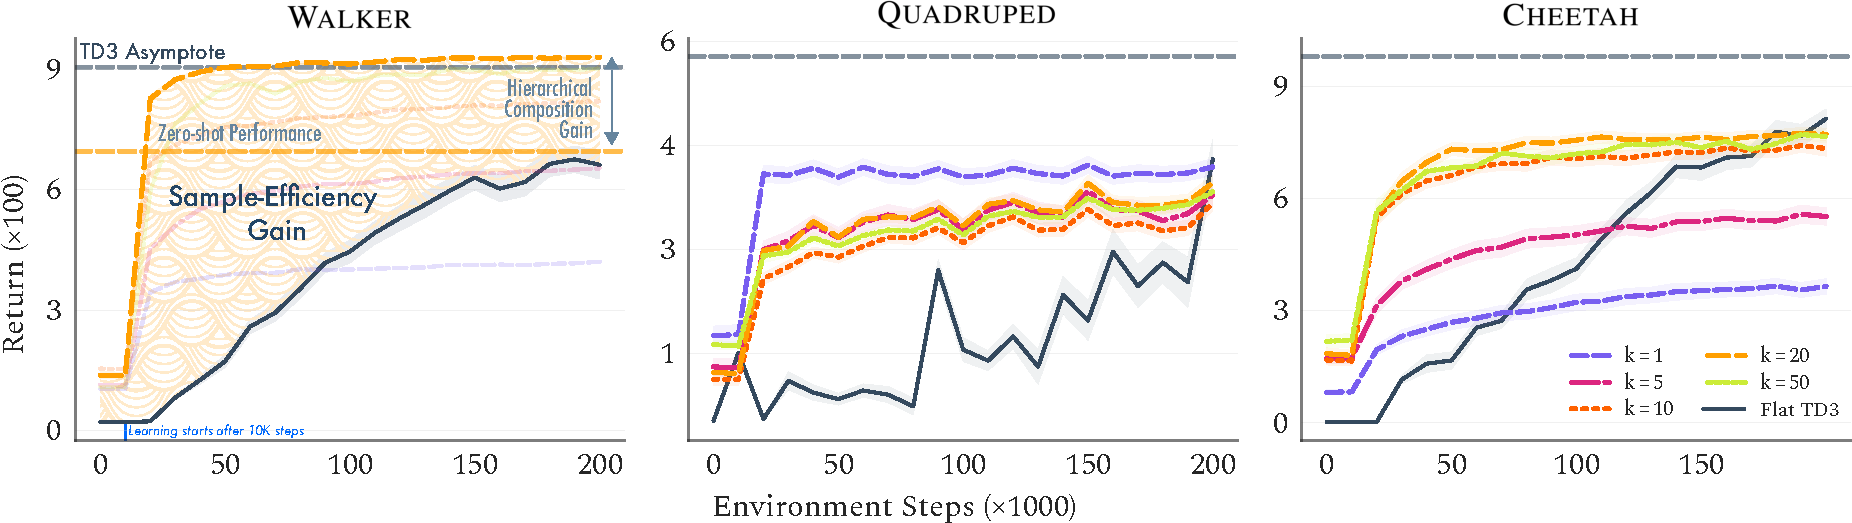
\includegraphics[width=\textwidth]{lk-curves-main.pdf}}
\caption{Evaluation curves for LK with varying basis sizes and a flat TD3 agent on the \texttt{Walk} task, averaged over 30 independent runs for each of the three datasets (90 runs total per curve).}
\vspace{-5pt}
\label{fig:lk-curve-main}
\end{figure*}



Figure~\ref{fig:lk-curve-main} presents evaluation curves for LK and the flat TD3 on a representative task, \texttt{Walk}, across all three domains; the remaining curves are provided in the Appendix~\ref{sec:hier-comp-appendix}. We analyze the hierarchical advantages of LK in more detail in the \textsc{Walker} domain with $k=20$. The yellow shaded region indicates the sample-efficiency advantage of LK relative to the flat baseline. Both agents perform random exploration for the first 10K steps, after which learning begins. Despite operating in a higher-dimensional action space (dimension $k$) than the flat agent (domain-specific action dimension, 6 in \textsc{Walker}), LK exhibits rapid performance gains and converges to a stable policy earlier. This behavior is consistent with the hypothesis outlined in Section~\ref{sec:downstream}. We additionally indicate the hierarchical composition gain, defined as the improvement of LK over its zero-shot performance, corresponding to the values reported in Table~\ref{tab:perc_imp_fb_lk}.
\looseness = -1


\section{Comparison Against Privileged Baseline}
~\label{sec:exp_alegre}
\vspace{-10pt}

As a final empirical evaluation, we compare LK to Option Keyboard Basis \citep[OKB;][]{alegre2025constructing}. OKB constructs its option basis from environment-provided reward features that span downstream tasks and is theoretically guaranteed to recover a basis sufficient for optimal control. This comparison assesses whether LK can achieve competitive performance without access to such privileged, handcrafted reward information, thereby highlighting the effectiveness of the Laplacian behavior basis.

We evaluate on the \textsc{Item-Collector} task \cite{barreto2019option, alegre2025constructing}, a $10\times10$ toroidal gridworld where the agent must collect items in a fixed order. Transitions are annotated with reward features for OKB, while LK is pre-trained on a reward-free dataset collected via a uniform random walk. The USFA is trained with Double DQN \citep{van2016deep} using basis sizes $k \in \{20,30,40\}$. Zero-shot performance is evaluated with 50K labeled samples, and the meta-policy is trained for 500K steps.

Figure~\ref{fig:okb_comp} compares the evaluation returns of OKB and LK. Despite relying only on transition data and lacking privileged reward features, LK achieves performance close to OKB. With more training steps, we observe that the gap between OKB and LK decreases, indicating that LK can recover structural information from environment dynamics alone to induce effective behaviors. More generally, it suggests that strong downstream performance does not require explicit reward-feature engineering, as Laplacian eigenvectors form a scalable basis for reusable options.


\section{Conclusion}

We establish both theoretically and empirically that graph Laplacian eigenvectors form a principled and sample-efficient basis for RL. When combined with a USFA, they induce a task-agnostic behavior basis that can be queried to solve a range of downstream tasks, effectively functioning as a behavioral foundation model. However, as highlighted by the big world hypothesis~\citep{javed2024big}, no fixed basis can capture the full diversity of tasks in large and complex environments. To address this limitation, we introduce the Laplacian Keyboard, a hierarchical framework in which a meta-policy adapts the fixed behavior basis to a given task through sequential composition at execution time. As noted by \citet{javed2024big}, \textit{``the key research challenge for achieving goals in big worlds is to come up with solution methods that efficiently utilize the limited resources of the agent"}; LK follows this principle by treating the learned basis as a structured starting point rather than a complete solution. Empirical results across multiple environments and basis sizes demonstrate improved performance over zero-shot baselines and greater sample efficiency than flat RL agents. \looseness = -1



\begin{figure}[t]
\centerline{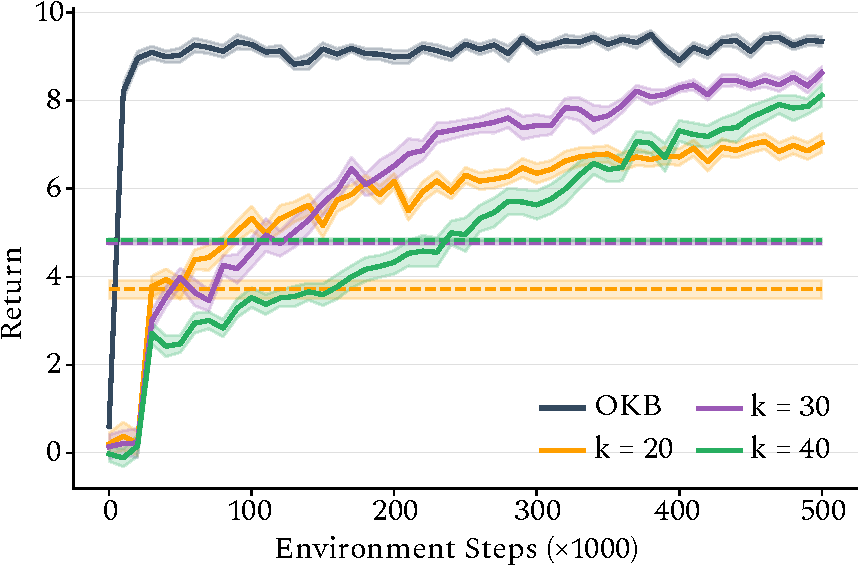
\includegraphics[width=.8\columnwidth]{okb.pdf}}
\caption{Evaluation curves for LK with varying basis sizes and OKB, averaged over 30 independent runs. The shaded region indicates the standard error. The horizontal dashed line corresponds to the zero-shot performance.}
\label{fig:okb_comp}
\vspace{-15pt}
\end{figure}

While this work focuses on an offline, reward-free setting, a natural extension is a fully online framework in which representation-driven option discovery~\citep{machado2023temporal, klissarov2023deep} is combined with LK to support efficient exploration and continual refinement of the behavior basis. We also observe that tasks favor different option termination horizons \(t_{\text{term}}\), suggesting that learning termination sets could further improve temporal abstraction and meta-policy adaptation.


\section*{Impact Statement}
This paper presents work whose goal is to advance the field
of Reinforcement Learning. There are many potential societal
consequences of our work, none which we feel must be
specifically highlighted here.

\bibliography{references.bib}
% \bibliographystyle{icml2026}


\begin{thebibliography}{39}
\providecommand{\natexlab}[1]{#1}
\providecommand{\url}[1]{\texttt{#1}}
\expandafter\ifx\csname urlstyle\endcsname\relax
  \providecommand{\doi}[1]{doi: #1}\else
  \providecommand{\doi}{doi: \begingroup \urlstyle{rm}\Url}\fi

\bibitem[Agarwal et~al.(2025{\natexlab{a}})Agarwal, Chuck, Sikchi, Hu, Rudolph, Niekum, Stone, and Zhang]{agarwal2025unified}
Agarwal, S., Chuck, C., Sikchi, H., Hu, J., Rudolph, M., Niekum, S., Stone, P., and Zhang, A.
\newblock {A Unified Framework for Unsupervised Reinforcement Learning Algorithms}.
\newblock In \emph{Workshop on Reinforcement Learning Beyond Rewards@ Reinforcement Learning Conference}, 2025{\natexlab{a}}.

\bibitem[Agarwal et~al.(2025{\natexlab{b}})Agarwal, Sikchi, Stone, and Zhang]{agarwal2025proto}
Agarwal, S., Sikchi, H., Stone, P., and Zhang, A.
\newblock {Proto Successor Measure: Representing the Behavior Space of an RL Agent}.
\newblock In \emph{{International Conference on Machine Learning}}, 2025{\natexlab{b}}.

\bibitem[Alegre et~al.(2025)Alegre, Bazzan, Barreto, and Da~Silva]{alegre2025constructing}
Alegre, L.~N., Bazzan, A. L.~C., Barreto, A., and Da~Silva, B.~C.
\newblock {Constructing an Optimal Behavior Basis for the Option Keyboard}.
\newblock In \emph{{Neural Information Processing Systems}}, 2025.

\bibitem[Alver \& Precup(2022)Alver and Precup]{alver2022sip}
Alver, S. and Precup, D.
\newblock {Constructing a Good Behavior Basis for Transfer using Generalized Policy Updates}.
\newblock In \emph{International Conference on Learning Representations}, 2022.

\bibitem[Bagatella et~al.(2025)Bagatella, Pirotta, Touati, Lazaric, and Tirinzoni]{bagatella2025tdjepa}
Bagatella, M., Pirotta, M., Touati, A., Lazaric, A., and Tirinzoni, A.
\newblock {TD-JEPA: Latent-predictive Representations for Zero-Shot Reinforcement Learning}.
\newblock \emph{arXiv preprint arXiv:2510.00739}, 2025.

\bibitem[Barreto et~al.(2017)Barreto, Dabney, Munos, Hunt, Schaul, van Hasselt, and Silver]{barreto2017successor}
Barreto, A., Dabney, W., Munos, R., Hunt, J.~J., Schaul, T., van Hasselt, H., and Silver, D.
\newblock {Successor Features for Transfer in Reinforcement Learning}.
\newblock In \emph{{Neural Information Processing Systems}}, 2017.

\bibitem[Barreto et~al.(2019)Barreto, Borsa, Hou, Comanici, Ayg{\"u}n, Hamel, Toyama, Mourad, Silver, and Precup]{barreto2019option}
Barreto, A., Borsa, D., Hou, S., Comanici, G., Ayg{\"u}n, E., Hamel, P., Toyama, D., Mourad, S., Silver, D., and Precup, D.
\newblock {The Option Keyboard: Combining Skills in Reinforcement Learning}.
\newblock In \emph{{Neural Information Processing Systems}}, 2019.

\bibitem[Barreto et~al.(2020)Barreto, Hou, Borsa, Silver, and Precup]{barreto2020fast}
Barreto, A., Hou, S., Borsa, D., Silver, D., and Precup, D.
\newblock {Fast Reinforcement Learning with Generalized Policy Updates}.
\newblock \emph{{Proceedings of the National Academy of Sciences}}, 117\penalty0 (48):\penalty0 30079--30087, 2020.

\bibitem[Bellemare et~al.(2019)Bellemare, Dabney, Dadashi, Ali~Taiga, Castro, Le~Roux, Schuurmans, Lattimore, and Lyle]{bellemare2019geometric}
Bellemare, M., Dabney, W., Dadashi, R., Ali~Taiga, A., Castro, P.~S., Le~Roux, N., Schuurmans, D., Lattimore, T., and Lyle, C.
\newblock {A Geometric Perspective on Optimal Representations for Reinforcement Learning}.
\newblock \emph{Neural Information Processing Systems}, 2019.

\bibitem[Blier et~al.(2021)Blier, Tallec, and Ollivier]{blier2021learning}
Blier, L., Tallec, C., and Ollivier, Y.
\newblock {Learning Successor States and Goal-Dependent Values: A Mathematical Viewpoint}.
\newblock \emph{{arXiv preprint arXiv:2101.07123}}, 2021.

\bibitem[Borsa et~al.(2019)Borsa, Barreto, Quan, Mankowitz, van Hasselt, Munos, Silver, and Schaul]{borsauniversal}
Borsa, D., Barreto, A., Quan, J., Mankowitz, D.~J., van Hasselt, H., Munos, R., Silver, D., and Schaul, T.
\newblock {Universal Successor Features Approximators}.
\newblock In \emph{{International Conference on Learning Representations}}, 2019.

\bibitem[Carvalho et~al.(2023)Carvalho, Saraiva, Filos, Lampinen, Matthey, Lewis, Lee, Singh, Jimenez~Rezende, and Zoran]{carvalho2023combining}
Carvalho, W., Saraiva, A., Filos, A., Lampinen, A., Matthey, L., Lewis, R.~L., Lee, H., Singh, S., Jimenez~Rezende, D., and Zoran, D.
\newblock {Combining Behaviors with the Successor Features Keyboard}.
\newblock In \emph{{Neural Information Processing Systems}}, 2023.

\bibitem[Chandrasekar \& Machado(2025)Chandrasekar and Machado]{chandrasekar2025towards}
Chandrasekar, S. and Machado, M.~C.
\newblock {Towards An Option Basis To Optimize All Rewards}.
\newblock In \emph{Workshop on Reinforcement Learning Beyond Rewards@ Reinforcement Learning Conference}, 2025.

\bibitem[Dayan(1993)]{dayan1993improving}
Dayan, P.
\newblock {Improving Generalization for Temporal Difference Learning: The Successor Representation}.
\newblock \emph{Neural computation}, 5\penalty0 (4):\penalty0 613--624, 1993.

\bibitem[Fourier(1878)]{fourier1878analytical}
Fourier, J.
\newblock \emph{The Analytical Theory of Heat}.
\newblock {Cambridge University Press}, 1878.

\bibitem[Fujimoto et~al.(2018)Fujimoto, Hoof, and Meger]{fujimoto2018addressing}
Fujimoto, S., Hoof, H.~v., and Meger, D.
\newblock {Addressing Function Approximation Error in Actor-Critic Methods}.
\newblock In \emph{{International Conference on Machine Learning}}, 2018.

\bibitem[Gomez et~al.(2023)Gomez, Bowling, and Machado]{gomezproper}
Gomez, D., Bowling, M., and Machado, M.~C.
\newblock {Proper Laplacian Representation Learning}.
\newblock In \emph{{International Conference on Learning Representations}}, 2023.

\bibitem[Huang et~al.(2022)Huang, Dossa, Ye, Braga, Chakraborty, Mehta, and Araújo]{huang2022cleanrl}
Huang, S., Dossa, R. F.~J., Ye, C., Braga, J., Chakraborty, D., Mehta, K., and Araújo, J.~G.
\newblock {CleanRL: High-quality Single-file Implementations of Deep Reinforcement Learning Algorithms}.
\newblock \emph{{Journal of Machine Learning Research}}, 23\penalty0 (274):\penalty0 1--18, 2022.

\bibitem[Jajoo et~al.(2025)Jajoo, Sikchi, Agarwal, Zhang, Niekum, and White]{jajoo2025regularized}
Jajoo, P., Sikchi, H., Agarwal, S., Zhang, A., Niekum, S., and White, M.
\newblock {Regularized Latent Dynamics Prediction is a Strong Baseline for Behavioral Foundation Models}.
\newblock In \emph{Workshop on Reinforcement Learning Beyond Rewards@ Reinforcement Learning Conference}, 2025.

\bibitem[Javed \& Sutton(2024)Javed and Sutton]{javed2024big}
Javed, K. and Sutton, R.~S.
\newblock {The Big World Hypothesis and its Ramifications for Artificial Intelligence}.
\newblock In \emph{{Finding the Frame: An RLC Workshop for Examining Conceptual Frameworks}}, 2024.

\bibitem[Jinnai et~al.(2019)Jinnai, Park, Abel, and Konidaris]{jinnai2019discovering}
Jinnai, Y., Park, J.~W., Abel, D., and Konidaris, G.
\newblock {Discovering Options for Exploration by Minimizing Cover Time}.
\newblock In \emph{{International Conference on Machine Learning}}, pp.\  3130--3139, 2019.

\bibitem[Klissarov \& Machado(2023)Klissarov and Machado]{klissarov2023deep}
Klissarov, M. and Machado, M.~C.
\newblock {Deep Laplacian-Based Options for Temporally-Extended Exploration}.
\newblock In \emph{{International Conference on Machine Learning}}, 2023.

\bibitem[Levin \& Peres(2017)Levin and Peres]{levin2017markov}
Levin, D.~A. and Peres, Y.
\newblock \emph{{Markov Chains and Mixing Times}}, volume 107.
\newblock American Mathematical Soc., 2017.

\bibitem[Machado et~al.(2017)Machado, Bellemare, and Bowling]{machado2017laplacian}
Machado, M.~C., Bellemare, M.~G., and Bowling, M.
\newblock {A Laplacian Framework for Option Discovery in Reinforcement Learning}.
\newblock In \emph{{International Conference on Machine Learning}}, 2017.

\bibitem[Machado et~al.(2023)Machado, Barreto, Precup, and Bowling]{machado2023temporal}
Machado, M.~C., Barreto, A., Precup, D., and Bowling, M.
\newblock {Temporal Abstraction in Reinforcement Learning with the Successor Representation}.
\newblock \emph{{Journal of Machine Learning Research}}, 24\penalty0 (80):\penalty0 1--69, 2023.

\bibitem[Mahadevan(2005)]{mahadevan2005proto}
Mahadevan, S.
\newblock {Proto-Value Functions: Developmental Reinforcement Learning}.
\newblock In \emph{{International Conference on Machine Learning}}, pp.\  553--560, 2005.

\bibitem[Ollivier(2025)]{ollivier2025features}
Ollivier, Y.
\newblock {Which Features are Best for Successor Features?}
\newblock \emph{arXiv preprint arXiv:2502.10790}, 2025.

\bibitem[Park et~al.(2024)Park, Kreiman, and Levine]{park2024hilp}
Park, S., Kreiman, T., and Levine, S.
\newblock {Foundation Policies with Hilbert Representations}.
\newblock In \emph{International Conference on Machine Learning}, 2024.

\bibitem[Shuman et~al.(2016)Shuman, Ricaud, and Vandergheynst]{shuman2016vertex}
Shuman, D.~I., Ricaud, B., and Vandergheynst, P.
\newblock {Vertex-frequency Analysis on Graphs}.
\newblock \emph{Applied and Computational Harmonic Analysis}, 40\penalty0 (2):\penalty0 260--291, 2016.

\bibitem[Sikchi et~al.(2025)Sikchi, Tirinzoni, Touati, Xu, Kanervisto, Niekum, Zhang, Lazaric, and Pirotta]{sikchi2025fast}
Sikchi, H., Tirinzoni, A., Touati, A., Xu, Y., Kanervisto, A., Niekum, S., Zhang, A., Lazaric, A., and Pirotta, M.
\newblock {Fast Adaptation with Behavioral Foundation Models}.
\newblock In \emph{Reinforcement Learning Conference}, 2025.

\bibitem[Sutton et~al.(1999)Sutton, Precup, and Singh]{sutton1999between}
Sutton, R.~S., Precup, D., and Singh, S.
\newblock {Between MDPs and Semi-MDPs: A Framework for Temporal Abstraction in Reinforcement Learning}.
\newblock \emph{{Artificial Intelligence}}, 112\penalty0 (1-2):\penalty0 181--211, 1999.

\bibitem[Tassa et~al.(2018)Tassa, Doron, Muldal, Erez, Li, Casas, Budden, Abdolmaleki, Merel, Lefrancq, et~al.]{tassa2018deepmind}
Tassa, Y., Doron, Y., Muldal, A., Erez, T., Li, Y., Casas, D. d.~L., Budden, D., Abdolmaleki, A., Merel, J., Lefrancq, A., et~al.
\newblock {Deepmind Control Suite}.
\newblock \emph{arXiv preprint arXiv:1801.00690}, 2018.

\bibitem[Tirinzoni et~al.(2025{\natexlab{a}})Tirinzoni, Touati, Farebrother, Guzek, Kanervisto, Xu, Lazaric, and Pirotta]{tirinzoni2025zero}
Tirinzoni, A., Touati, A., Farebrother, J., Guzek, M., Kanervisto, A., Xu, Y., Lazaric, A., and Pirotta, M.
\newblock {Zero-shot Whole-body Humanoid Control via Behavioral Foundation Models}.
\newblock In \emph{{International Conference on Learning Representations}}, 2025{\natexlab{a}}.

\bibitem[Tirinzoni et~al.(2025{\natexlab{b}})Tirinzoni, Touati, Farebrother, Guzek, Kanervisto, Xu, Lazaric, and Pirotta]{tirinzonizero}
Tirinzoni, A., Touati, A., Farebrother, J., Guzek, M., Kanervisto, A., Xu, Y., Lazaric, A., and Pirotta, M.
\newblock {Zero-Shot Whole-Body Humanoid Control via Behavioral Foundation Models}.
\newblock In \emph{{International Conference on Learning Representations}}, 2025{\natexlab{b}}.

\bibitem[Touati et~al.(2023)Touati, Rapin, and Ollivier]{touati2022does}
Touati, A., Rapin, J., and Ollivier, Y.
\newblock {Does Zero-Shot Reinforcement Learning Exist?}
\newblock In \emph{{International Conference on Learning Representations}}, 2023.

\bibitem[van Hasselt et~al.(2016)van Hasselt, Guez, and Silver]{van2016deep}
van Hasselt, H., Guez, A., and Silver, D.
\newblock {Deep Reinforcement Learning with Double Q-learning}.
\newblock In \emph{AAAI Conference on Artificial Intelligence}, 2016.

\bibitem[Yarats et~al.(2022)Yarats, Brandfonbrener, Liu, Laskin, Abbeel, Lazaric, and Pinto]{yarats2022exorl}
Yarats, D., Brandfonbrener, D., Liu, H., Laskin, M., Abbeel, P., Lazaric, A., and Pinto, L.
\newblock {Don't Change the Algorithm, Change the Data: Exploratory Data for Offline Reinforcement Learning}.
\newblock \emph{arXiv preprint arXiv:2201.13425}, 2022.

\bibitem[Zahavy et~al.(2021)Zahavy, Barreto, Mankowitz, Hou, O'Donoghue, Kemaev, and Singh]{zahavy2021discovering}
Zahavy, T., Barreto, A., Mankowitz, D.~J., Hou, S., O'Donoghue, B., Kemaev, I., and Singh, S.
\newblock {Discovering a Set of Policies for the Worst Case Reward}.
\newblock In \emph{International Conference on Learning Representations}, 2021.

\bibitem[Zhu \& Rabbat(2012)Zhu and Rabbat]{zhu2012approximating}
Zhu, X. and Rabbat, M.
\newblock {Approximating Signals Supported on Graphs}.
\newblock In \emph{{IEEE International Conference on Acoustics, Speech and Signal Processing}}, 2012.

\end{thebibliography}



\newpage
\appendix
\onecolumn

\section{Extended Related Work}
\label{sec:extended-related-work}

The Laplacian Keyboard bridges representation-based and behavior-based solution methods to address the \textit{zero-shot} RL problem. In this section, we review closely related work along both directions, extending the discussion beyond that provided in the main paper. \looseness=-1

\paragraph{Representation-based Methods:}
A common approach to zero-shot RL is to learn task-agnostic state representations that can be reused for downstream control. Examples include Hilbert Foundation Policies \citep[HILP;][]{park2024hilp}, Proto Successor Measures \citep[PSM;][]{agarwal2025proto}, Regularized Latent Dynamics Prediction \citep[RLDP;][]{jajoo2025regularized}, and TD-JEPA \citep{bagatella2025tdjepa}. While these methods differ in their objectives, they all aim to construct representations that support policy transfer without additional environment interaction.

HILP learns representations sufficient for expressing goal-reaching value functions and uses them to construct intrinsic reward functions for training a latent-conditioned policy. PSM learns a basis over state visitation distributions, enabling downstream behaviors to be synthesized as linear combinations of these bases and supporting zero-shot policy construction via reward-dependent recombination. RLDP and TD-JEPA learn predictive latent representations by modeling future states while regularizing against feature collapse; these representations are then paired with USFA to enable zero-shot transfer. A unified treatment of several representation-based methods is provided by \citet{agarwal2025unified}.

Closely related in spirit to LK are the LoLa and ReLa algorithms proposed by \citet{sikchi2025fast}, which also exploit pre-trained knowledge to improve downstream task performance. However, unlike the LK, these methods are not hierarchical in nature and are primarily motivated by reducing approximation errors arising during pre-training and inference. As a result, they are better characterized as fine-tuning or correction mechanisms rather than frameworks for skill composition.

\paragraph{Behavior-based Methods:}

Set of Independent Policies \citep[SIP;][]{alver2022sip}, Set Max Policies \citep[SMP;][]{zahavy2021discovering}, and the Successor Feature Keyboard \citep[SFK;][]{carvalho2023combining} are few examples that focus on learning a reusable set of behaviors or policies to enable zero-shot control.

SIP assumes access to a set of independent reward features and learns a policy for each feature. At test time, GPE \& GPI are used to recover the optimal policy for any reward expressed as a linear combination of these features. SMP retains the linear reward assumption but optimizes for robustness by learning policies that maximize worst-case performance over admissible rewards; zero-shot transfer is again achieved using GPE \& GPI. SFK relaxes the assumption of known reward features and learns a policy basis by extracting shared structure across a set of training tasks.


\vspace{10pt}

A unifying backbone of these methods is the successor representation \citep[SR;][]{dayan1993improving} and its generalization, successor features \citep[SF;][]{barreto2017successor}. These frameworks decompose the value function into a dynamics-dependent component, capturing long-term state visitation, and a task-specific component defined by the reward. SR represents each state by its expected discounted future state occupancies under a policy, while SF extends this idea to feature spaces by modeling expected discounted feature activations. Under the assumption of linear reward functions, this decomposition allows value functions to be computed as inner products between SF and reward weights, naturally enabling zero-shot transfer via GPE \& GPI and USFA.



\newpage

\section{Laplacian Basis}

In this section, we provide the proof for Theorem \ref{theorem:the-one-main-paper}. We first provide the necessary background, followed by the proof. We reintroduce a few details for completeness. 

\subsection{Background}~\label{sec:app_background}

The proof and theorem is partly inspired from the spectral graph theory literature. Hence we first introduce concepts in the language of graph theory before using them for RL.

\subsubsection{Spectral Theory}
\label{apdx:gft_bg}

\paragraph{Graph Laplacian:} 

Consider an undirected graph $G = (\mathscr{V}, \mathscr{E})$ with vertex set $\mathscr{V}$ and edge set $\mathscr{E}$. Each edge $(i, j) \in \mathscr{E}$ carries a non-negative weight $w_{ij} \ge 0$ quantifying the connection strength between vertices $i$ and $j$. These weights define the weighted adjacency matrix $\mathbf{W} \in \mathbb{R}^{|\mathscr{V}| \times |\mathscr{V}|}$, where $\mathbf{W}_{ij} = w_{ij}$ for $(i, j) \in \mathscr{E}$ and $\mathbf{W}_{ij} = 0$ otherwise. The vertex degrees $d_i = \sum_j w_{ij}$ form the degree matrix $\mathbf{D} = \mathrm{diag}(d_1, d_2, \dots, d_{|\mathscr{V}|})$. For undirected graphs, the adjacency matrix exhibits symmetry: $w_{ij} = w_{ji} \, \forall (i, j) \in \mathscr{E}$.

The \textit{graph Laplacian matrix} is defined as $\mathbf{L} \, \dot{=} \, \mathbf{D} - \mathbf{W}$, a real symmetric positive semi-definite matrix admitting the eigendecomposition $\mathbf{L} = \mathbf{E} \mathbf{\Lambda} \mathbf{E}^\top$. Here, $\mathbf{E} = [\ei_1, \ei_2, \dots, \ei_{|\mathscr{V}|}]$ contains orthonormal eigenvectors and $\mathbf{\Lambda} = \mathrm{diag}(\lambda_1, \lambda_2, \dots, \lambda_{|\mathscr{V}|})$ contains the corresponding non-negative eigenvalues ordered such that $0 = \lambda_1 \le \lambda_2 \le \cdots \le \lambda_{|\mathscr{V}|}$. These eigenvectors encode structural properties of the graph in an ordered fashion: eigenvectors associated with smaller eigenvalues (low frequencies) exhibit smooth variations across the graph, while those associated with larger eigenvalues (high frequencies) capture rapid oscillations between neighboring vertices. \looseness = -1


\paragraph{Graph Fourier Transform:} 
Any graph signal $f: \mathscr{V} \rightarrow \mathbb{R}$ defined over the vertices admits an exact decomposition as a linear combination of the Laplacian eigenvectors:
\begin{equation}
\mathbf{f} = \sum_{i=1}^{|\mathscr{V}|} \hat{f}_i \ei_i,
\end{equation}
where the \textit{Graph Fourier coefficients} $\hat{f}_i = \langle \mathbf{f}, \ei_i \rangle$ represent the projection of $\mathbf{f}$ onto the $i$-th eigenvector. The \textit{Graph Fourier Transform} (GFT) $\mathbf{\hat{f}} = \mathbf{E}^\top \mathbf{f}$ maps signals from the vertex domain to the spectral domain, where $\mathbf{\hat{f}} = [\hat{f}_1, \hat{f}_2, \dots, \hat{f}_{|\mathscr{V}|}]^\top$ denotes the signal's spectral representation. This transformation serves as the graph analog of the classical Fourier transform, decomposing arbitrary graph signals into fundamental frequency components. Signals dominated by small coefficients $\hat{f}_i$ for low $i$ vary smoothly across the graph topology, while those with significant high-index coefficients exhibit complex, irregular patterns that vary sharply between connected vertices. \looseness = -1

A fundamental property of the GFT is energy preservation across domains, formalized by Parseval's theorem \cite{shuman2016vertex}:

\begin{lemma}[Parseval's Theorem]
The energy of a signal in the vertex domain equals its energy in the spectral domain:
\begin{equation}
\sum_{i=1}^{|\mathscr{V}|} f(i)^2 = \sum_{i=1}^{|\mathscr{V}|} \hat{f}_i^2.
\end{equation}
\label{lm:parseval}
\end{lemma}

This property allows us to measure energy of the signal as a function of the Graph Fourier coefficients.

\paragraph{Truncated Spectral Approximation:} 
For large graphs where $|\mathscr{V}|$ is large, computing and storing the full basis becomes computationally prohibitive. This constraint requires restricting the representation to a \textit{truncated spectral basis} consisting of the first $k \ll |\mathscr{V}|$ eigenvectors corresponding to the smallest eigenvalues. The resulting approximation
\begin{equation}
\mathbf{f}_k = \sum_{i=1}^{k} \hat{f}_i \ei_i
\end{equation}
captures the signal's low-frequency components---variations that are smooth with respect to the graph structure. This dimensionality reduction induces an inductive bias toward smoother signals that vary gradually across connected vertices while filtering out high-frequency fluctuations. The truncation sacrifices exact reconstruction in favor of computational efficiency. \looseness = -1

The approximation error induced by truncation can be quantified through Parseval's theorem. Since the omitted eigenvectors correspond to the high-frequency components, the squared reconstruction error is given by
\begin{equation}
    \operatorname{error}(f,k) \dot{=} \sum_{i = k+1}^{|\mathscr{V}|} \hat{f}_i^2,
\end{equation}
representing the energy concentrated in the discarded frequencies. This quantity measures the information loss incurred by restricting the reconstruction space to the subspace spanned by the first $k$ eigenvectors. As $k$ increases, the approximation error decreases, tightening the reconstruction quality.

\paragraph{Graph Signal Smoothness:} 
To formalize the notion of smoothness for signals defined over graphs, we rely on the \textit{graph total variation}, which quantifies local variations weighted by edge connectivity \citep{zhu2012approximating}.

\begin{definition}[Graph Total Variation]
For any graph signal $f: \mathscr{V} \to \mathbb{R}$, the graph total variation is defined as
\begin{equation}
    \|f\|_G \, \dot{=} \, \left[ \frac{1}{2}  \sum_{(i,j) \in \mathscr{E}} w_{ij} (f(i) - f(j))^2\right]^{\frac{1}{2}}.    
\end{equation}
\end{definition}

The graph total variation penalizes differences between signal values at connected vertices, weighted by their edge strengths. Smaller values of $\|f\|_G$ indicate that the signal varies smoothly across connected vertices. The factor $\frac{1}{2}$ accounts for double-counting in undirected graphs; \citet{zhu2012approximating} omit this term by enumerating each edge exactly once. 

A signal $f$ exhibits \textit{bounded variation} if there exists a constant $0 < C \ll \lambda_{|\mathscr{V}|}$ satisfying
\begin{equation}
\|f\|_G^2 \le C \cdot \|f\|^2,
\label{eqn:bounded_variation}
\end{equation}
where $\|f\|$ denotes the standard $\ell_2$ norm of $f$ viewed as a vector over the vertices.. This condition ensures that the signal exhibits controlled variability with respect to the underlying graph topology. The reconstruction error induced by truncation can be bounded using this smoothness measure,

\begin{lemma}[Reconstruction Bound \cite{zhu2012approximating}] 
For any signal $f$ with bounded variation, the squared reconstruction error using the first $k$ eigenvectors satisfies
\begin{equation}
    \operatorname{error}(f,k) \le \|f\|_G^2 \cdot \lambda_k^{-1}.
\end{equation}
\label{lm:error_bound}
\end{lemma}

The bound reveals two key factors influencing approximation quality. (1) Signals that vary smoothly over the graph structure, reflected by smaller $\|f\|_G$, incur smaller errors. (2) Increasing the basis size improves reconstruction: as $k$ grows, the corresponding eigenvalue $\lambda_k$ increases, tightening the bound. Together, they characterize how signal smoothness and basis dimensionality jointly determine reconstruction accuracy. \looseness = -1

\subsubsection{Laplacian for RL}
The spectral framework introduced above extends naturally to a class of MDPs known as reversible MDPs.

\paragraph{Reversible MDPs:} 
A Markov chain with state space $\mathscr{X}$ and transition matrix $\mathbf{P}$ is \textit{reversible} \citep{levin2017markov} if there exists a probability distribution $\pi$ on $\mathscr{X}$ satisfying the \textit{detailed balance equations}:
\[
\pi(x) P(x, y) = \pi(y) P(y, x) \quad \forall \, x, y \in \mathscr{X}.
\]
In the RL context, we call a policy $\pi$ reversible if the Markov chain it induces is reversible. Let $\pp(s, s') \, \dot{=} \, \sum_{a \in \mathscr{A}} \pi(a \mid s)\, p(s' \mid s, a)$ denote the policy-induced transition matrix. Then $\pi$ is reversible if the detailed balance condition holds: $\pp(s, s') = \pp(s', s) \, \forall \, s, s' \in \mathscr{S}$.

\paragraph{Graph Laplacian for Reversible MDPs:} 
Reversible MDPs can be modeled as undirected graphs $G = (\mathscr{S}, \mathscr{E})$, where the state space $\mathscr{S}$ forms the vertex set and edges represent feasible transitions. An edge $(s, s') \in \mathscr{E}$ exists whenever the transition probability between states $s$ and $s'$ is nonzero under policy $\pi$. The edge weight is defined as
\[
w_{ss'} \, \dot{=} \, \pp(s, s') = \sum_{a \in \mathscr{A}} \pi(a \mid s)\, p(s' \mid s, a),
\]
quantifying the policy-induced transition probability. For reversible policies, the adjacency matrix $\mathbf{W}$ is symmetric by construction, and the degree matrix reduces to the identity matrix $\mathbf{D} = \mathbf{I}$ since each row of $\pp$ sums to one.

The graph Laplacian is defined as $\mathbf{L} \, \dot{=} \, \mathbf{I} - \pp$, where $\pp$ denotes the state transition probability matrix. This formulation preserves the spectral properties established in Appendix~\ref{apdx:gft_bg}: $\mathbf{L}$ remains positive semi-definite with eigenvalues $0 = \lambda_1 \leq \lambda_2 \leq \cdots \leq \lambda_{|\mathscr{S}|}$, and its eigenvectors $\{\ei_i\}_{i=1}^{|\mathscr{S}|}$ form an orthonormal basis for functions defined over the state space.

\paragraph{Spectral Approximation of Reward Functions:} 
The primary graph signals of interest in RL are the reward function $r: \mathscr{S} \to \mathbb{R}$ and the value function $v: \mathscr{S} \to \mathbb{R}$. When these functions exhibit bounded variation with respect to the state space---meaning that states with high transition probability tend to have similar rewards or values---they can be efficiently approximated using a truncated Laplacian basis. In this work, we focus on the spectral representation of reward functions. Any reward function $r: \mathscr{S} \to \mathbb{R}$ admits the approximation
\begin{equation}
    \mathbf{r}_k = \sum_{i=1}^{k} \langle \mathbf{r}, \ei_i \rangle \, \ei_i,
\end{equation}
where the first $k$ eigenvectors capture the low-frequency components of the reward signal. This truncated basis restricts the representable reward space to smooth functions that vary gradually across connected states, filtering out high-frequency reward structures that exhibit sharp variations in the state space. \looseness = -1


\subsection{Formal Proof}
\label{sec:proof}

With the necessary background established, we now bound the change in the optimal value function caused by using an approximated reward function.

\begin{theorem}[\ValueApproxName \, (restated)]
Let $r: \mathscr{S} \to \mathbb{R}$ be a reward function with bounded variation and $\mathbf{r}_k$ its reconstruction using the first $k$ eigenvectors. Let $\mathbf{v}^*$ and $\mathbf{v}^*_k$ be their corresponding optimal value functions. Then,
\begin{equation}
    \|\mathbf{v}^* - \mathbf{v}^*_k\|_\infty \le \frac{\|r\|_G}{(1-\gamma)\sqrt{\lambda_k}},
\end{equation}
where $\lambda_k$ is the $k$-th eigenvalue.
\end{theorem}

\begin{proof}
We establish the bound in two stages: first, we bound the approximation error $\|\mathbf{r} - \mathbf{r}_k\|_{\infty}$, then propagate this through the value function.

\textbf{Step 1: Bounding the Signal Approximation Error.}

Let $\mathbf{r}_{residual} = \mathbf{r} - \mathbf{r}_k$ denote the reconstruction residual. By Parseval's theorem (Lemma \ref{lm:parseval}), the $\ell_2$ error is
\begin{equation}
    \|\mathbf{r} - \mathbf{r}_k\|_2^2 = \sum_s (r(s) - r_k(s))^2 = \sum_{i=k+1}^{|\mathscr{S}|} \hat{r}_i^2,
\end{equation}

where $\hat{r}_i$ is the $i$-th Graph Fourier coefficient. Applying Lemma \ref{lm:error_bound}, we obtain
\begin{equation}
    \|\mathbf{r} - \mathbf{r}_k\|_2^2 \leq \frac{\|r\|_G^2}{\lambda_k}.
\end{equation}
Since the $\ell_{\infty}$ norm is bounded by the $\ell_2$ norm, i.e., $\|\mathbf{r} - \mathbf{r}_k\|_{\infty}^2 \leq \|\mathbf{r} - \mathbf{r}_k\|_2^2$, we have
\begin{equation}
    \|\mathbf{r} - \mathbf{r}_k\|_{\infty} \leq \frac{\|r\|_G}{\sqrt{\lambda_k}} \coloneq \xi.
    \label{eq:approximation_error}
\end{equation}

\textbf{Step 2: Propagating Error Through the Value Function.}

Let $v^*$ and $v_k^*$ be the optimal value functions of $r$ and $r_k$. By the Bellman optimality equation:
\begin{equation}
    v^*(s) = \max_{a \in \mathscr{A}} \sum_{s' \in \mathscr{S}} p(s'|s,a) \left[ r(s') + \gamma v^*(s') \right]
\end{equation}

To bound the difference $\|v^* - v_k^*\|_\infty$, we start with the point-wise difference:
\begin{align}
    v^*(s) - v_k^*(s) &= \max_a \left[ \sum_{s'} p(s'|s,a) (r(s') + \gamma v^*(s')) \right] - \max_a \left[ \sum_{s'} p(s'|s,a) (r_k(s') + \gamma v_k^*(s')) \right] \notag \\
    &\leq \max_a \left[ \sum_{s'} p(s'|s,a) \left( (r(s') - r_k(s')) + \gamma(v^*(s') - v_k^*(s')) \right) \right]
\end{align}
where we used the property $\max_a f(a) - \max_a g(a) \leq \max_a (f(a) - g(a))$. 

Taking the supremum over $s \in \mathscr{S}$ on both sides:
\begin{align}
    \|\mathbf{v}^* - \mathbf{v}_k^*\|_{\infty} &\leq \left\| \max_a \sum_{s'} p(s'|s,a) \left[ (r(s') - r_k(s')) + \gamma(v^*(s') - v_k^*(s')) \right] \right\|_\infty \notag \\
    &\leq \max_{s,a} \sum_{s'} p(s'|s,a) \left| r(s') - r_k(s') \right| + \gamma \max_{s,a} \sum_{s'} p(s'|s,a) \left| v^*(s') - v_k^*(s') \right|
\end{align}

Since $\sum_{s'} p(s'|s,a) = 1$, the weighted average is bounded by the maximum difference:
\begin{equation}
    \sum_{s'} p(s'|s,a) |r(s') - r_k(s')| \leq \|\mathbf{r} - \mathbf{r}_k\|_{\infty} \quad \text{and} \quad \sum_{s'} p(s'|s,a) |v^*(s') - v_k^*(s')| \leq \|\mathbf{v}^* - \mathbf{v}_k^*\|_{\infty}
\end{equation}

Substituting these back into our inequality, we obtain:
\begin{equation}
    \|\mathbf{v}^* - \mathbf{v}_k^*\|_{\infty} \leq \|\mathbf{r} - \mathbf{r}_k\|_{\infty} + \gamma \|\mathbf{v}^* - \mathbf{v}_k^*\|_{\infty}
\end{equation}


Rearranging yields
\begin{equation}
    (1 - \gamma) \|\mathbf{v}^* - \mathbf{v}_k^*\|_{\infty} \leq \|\mathbf{r} - \mathbf{r}_k\|_{\infty}.
\end{equation}

\begin{equation}
    \|\mathbf{v}^* - \mathbf{v}_k^*\|_{\infty} \leq \frac{\|\mathbf{r} - \mathbf{r}_k\|_{\infty}}{(1 - \gamma)}.
    \label{eqn:tighter-bound}
\end{equation}

Note that when the reward function lies in the span of the first $k$ eigenvectors, exact reconstruction holds ($r = r_k$), yielding zero error.  More generally, this upper bound can be expressed in terms of the graph total variation. Substituting the bound from Equation~\ref{eq:approximation_error}:

\begin{equation}
    \|\mathbf{v}^* - \mathbf{v}_k^*\|_{\infty} \leq \frac{\xi}{1-\gamma} = \frac{\|r\|_G}{(1-\gamma)\sqrt{\lambda_k}}.
    \label{eqn:looser-bound}
\end{equation}

Finally, we note that the bound in Eqn. \ref{eqn:looser-bound} is looser, but it offers a more direct interpretation than the bound in Eqn. \ref{eqn:tighter-bound}. This concludes the proof.

\end{proof}

\subsection{Empirical Evaluation of Theorem~\ref{theorem:the-one-main-paper}}

Figure~\ref{fig:emperical-proof} illustrates an empirical evaluation in the \texttt{Four-Rooms} domain using four simple reward functions. We measure the approximation error of the resulting value function as a function of the basis size used to reconstruct the reward. The reward associated with any transition $(s,a,s')$ depends solely on the successor state $s'$, and episodes terminate upon reaching the designated bright red states.

The basis is formed by eigenvectors induced by a uniform random policy, and value functions are computed via value iteration. Across all settings, the proposed bound constitutes a strict upper bound on the observed value approximation error. As the basis size increases, the gap between the bound and the empirical error consistently decreases. Additionally, reward functions that vary smoothly over the state space exhibit substantially lower approximation error than noisier reward functions, highlighting the bias induced by using a truncated basis.

\begin{figure*}[t]
\centerline{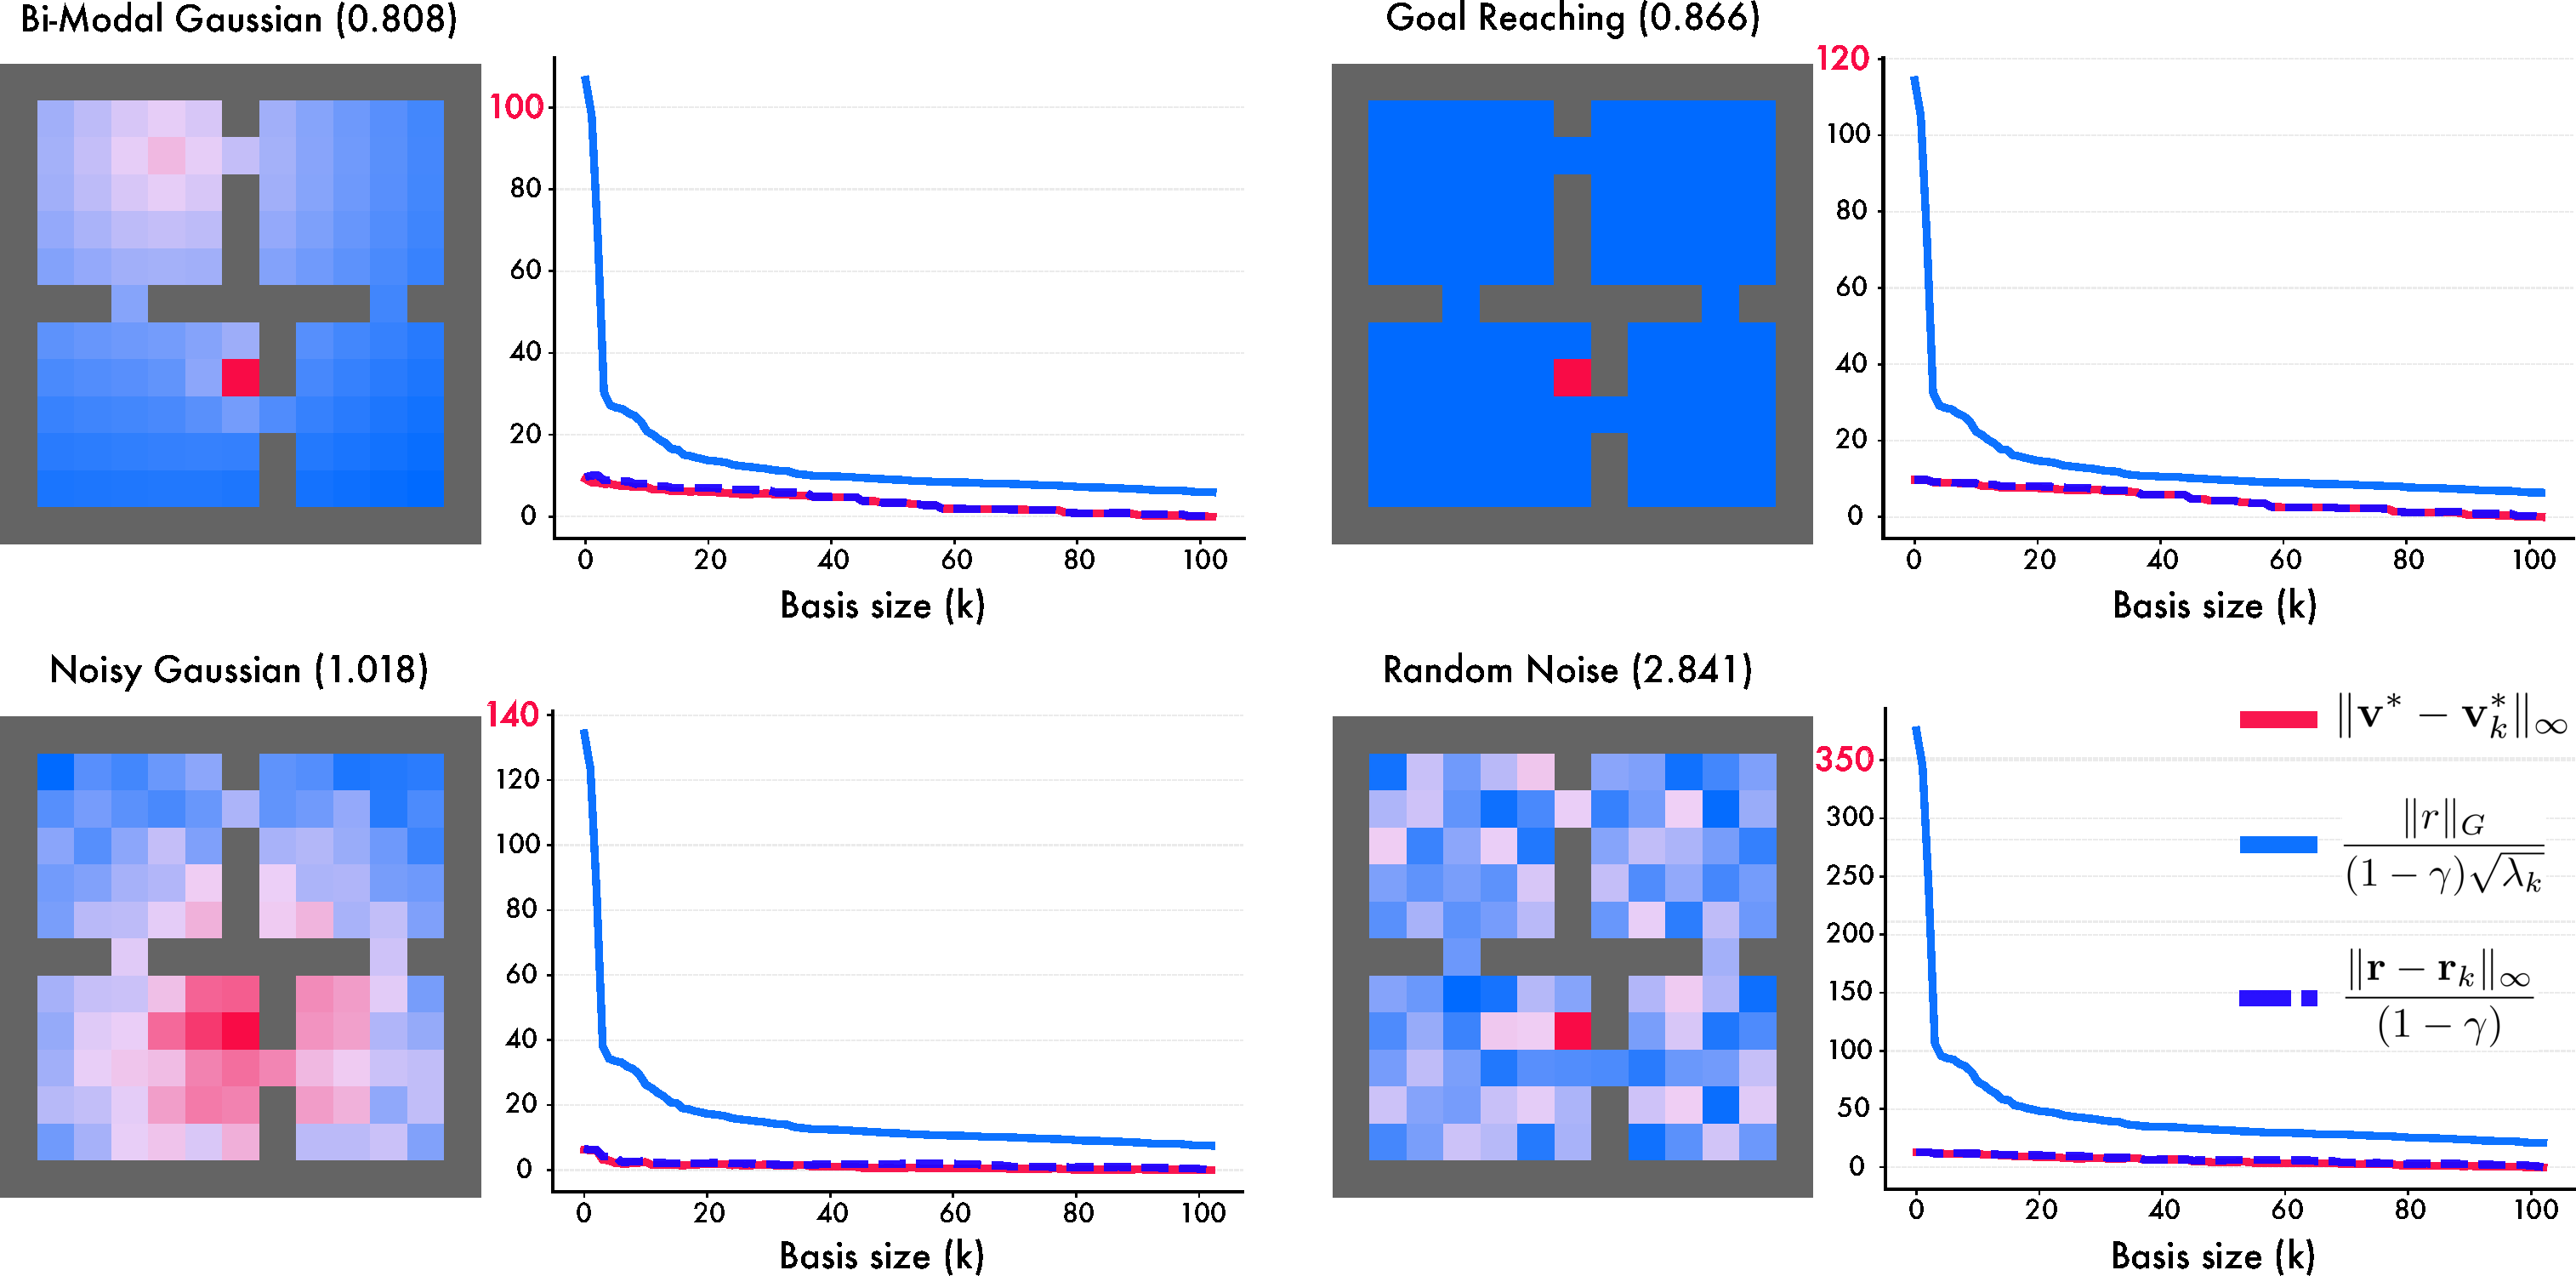
\includegraphics[width=\textwidth]{theorem_emperical.pdf}}
\caption{Reward reconstruction and induced value function error in \texttt{Four-Rooms}.
For four reward functions of increasing complexity (shown insets), we plot the value error, two different errors (Equation~\ref{eqn:tighter-bound} and ~\ref{eqn:looser-bound}) as a function of basis size $k$. The value in parenthesis corresponds to the reward function's graph norm. This environment has a total of 104 states.}
\label{fig:emperical-proof}
\end{figure*}


\newpage

\section{Experimental Details}
\label{sec:addn_exp}

We provide more experimental details in this section for clarity and reproducibility.


\subsection{Environments}
\label{sec:environments}

\textbf{DeepMind Control} (DMC) Suite \citep{tassa2018deepmind} comprises a variety of continuous control domains; in this work, we focus on three specific domains.

\begin{itemize}

    \item \textsc{Cheetah} is a bipedal agent actuated through a 6-dimensional continuous action space corresponding to joint torques. The observation space is 17-dimensional and consists of joint positions and joint velocities. In the \texttt{Walk} and \texttt{Run} tasks, the reward is a linear tolerance function of the forward torso velocity, encouraging the agent to exceed a task-specific speed threshold. The \texttt{Walk-Backward} and \texttt{Run-Backward} tasks are defined analogously by reversing the direction of the velocity term, thereby incentivizing backward locomotion.

    \item \textsc{Quadruped} is a four-legged agent actuated through a 12-dimensional continuous action space corresponding to joint torques. The observation space is 78-dimensional and consists of egocentric joint states, torso motion, inertial measurements, and force--torque readings at the feet. In the \texttt{Stand} task, the reward is a linear tolerance function encouraging an upright torso. The \texttt{Jump} task additionally rewards the agent for raising its center of mass above a target height while maintaining an upright posture. In the \texttt{Walk} and \texttt{Run} tasks, the reward is the product of the uprightness term and a forward-velocity term, incentivizing the agent to move at a task-specific target speed while remaining upright.

    \item \textsc{Walker} is a planar bipedal agent actuated through a 6-dimensional continuous action space corresponding to joint torques. The observation space is 24-dimensional and consists of body orientations, torso height, and joint velocities. In the \texttt{Run} tasks, the reward is a linear tolerance function of the horizontal torso velocity, encouraging the agent to achieve a target forward or backward speed. In the \texttt{Flip} tasks, the reward is instead defined over the torso’s angular momentum magnitude, incentivizing rapid rotational motion independent of translational velocity.




\end{itemize}

Across all DMC domains, tasks share the same underlying dynamics and differ only in their reward functions. Episodes have a fixed horizon of 1000 timesteps without early termination, yielding a maximum episode return close to 1000. We measure the undiscounted return, corresponding to setting $\gamma = 1$, as the performance metric.

\begin{figure*}[t]
\centerline{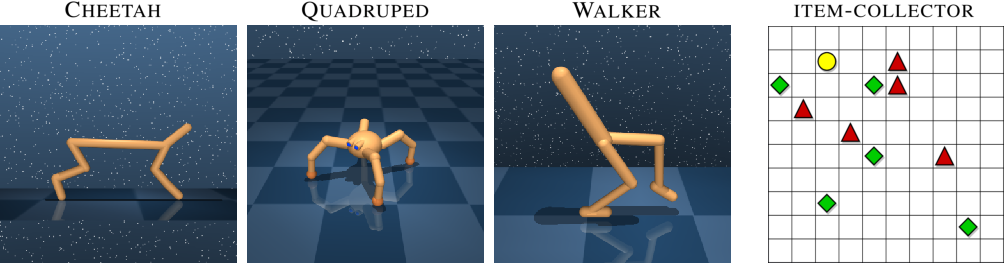
\includegraphics[width=.8\textwidth]{environments.pdf}}
\caption{The 4 environments we use to empirically evaluate the Laplacian Keyboard.}
\label{fig:environments}
\end{figure*}


\vspace{20pt}
\textbf{\textsc{Item-Collector}} is a discrete grid-world environment originally introduced by \citet{barreto2019option} and later used in \citet{alegre2025constructing} (Figure~\ref{fig:environments}). The environment consists of a $10 \times 10$ toroidal grid and a discrete action space of four cardinal movements. At the beginning of each episode, five items of each of two distinct types are placed uniformly at random across the grid. The agent’s objective is to collect all items of one type before collecting those of the other. Episodes terminate after 50 timesteps and admit a maximum undiscounted return of 10. The privileged reward features are two-dimensional and indicate which item type, if any, is collected at each transition. Performance is evaluated using the undiscounted return, corresponding to a discount factor of $\gamma = 1$.


\newpage

\subsection{Training Details}

\paragraph{Laplacian Encoder:}
The Laplacian Encoder is trained using ALLO, the contrastive objective shown in Equation~\ref{eqn:allo}:

\begin{equation}
\max_{\boldsymbol{\beta}} \min_{\mathbf{u} \in \mathbb{R}^{k|\mathscr{S}|}}
\underbrace{
  \sum_{i=1}^k \langle \mathbf{u}_i, \mathbf{L}\mathbf{u}_i \rangle
}_{\text{smoothness}}
+
\underbrace{
  \sum_{j=1}^k \sum_{k=1}^j
  \Big[
    \beta_{jk}
    \big(
      \langle \mathbf{u}_j, \llbracket \mathbf{u}_k \rrbracket \rangle
      - \delta_{jk}
    \big)
    +
    b
    \big(
      \langle \mathbf{u}_j, \llbracket \mathbf{u}_k \rrbracket \rangle
      - \delta_{jk}
    \big)^2
  \Big]
}_{\text{orthogonality constraints}}
\tag{3}
\label{eqn:allo}
\end{equation}

Each training batch consists of a positive pair of states and a negative state. The positive pair is used to estimate the smoothness term, while the negative sample contributes to the orthogonality constraints. To construct a positive pair, we sample an episode and a reference state from that episode, and then sample a paired state according to a geometric distribution parameterized by $\gamma_{\text{allo}}$. The negative sample is drawn as another random state from the same episode. The Laplacian Encoder is trained via gradient descent and maps raw observations to a $k$-dimensional Laplacian representation.

\paragraph{Universal Successor Feature Approximators (USFA):}
USFA is trained as a value function, instantiated as the critic in a TD3 agent for continuous action spaces and as the Q-network in a Double DQN agent for discrete action spaces. We do not employ additional offline RL-specific techniques. To expose the USFA to a broad class of reward functions during pre-training, we sample weight vectors $\mathbf{w} \in \mathbb{R}^k$ following \citet{touati2022does}.
\begin{enumerate}
    \item Weight vectors sampled uniformly from the sphere of radius $\sqrt{k}$, corresponding to reward functions given by random linear combinations of the Laplacian eigenvectors.
    \item Weight vectors obtained by sampling a random state from the offline dataset and using its Laplacian representation as $\mathbf{w}$, corresponding to a goal-reaching reward with the sampled state as the goal.
\end{enumerate}
The actor takes the raw observation and the weight vector as input and outputs an action. The critic takes the raw observation, action, and weight vector as input and outputs the corresponding successor feature. Gradients from the USFA do not propagate into the Laplacian Encoder.

\paragraph{Zero-shot:}
After training the Laplacian encoder and the USFA, and given a downstream task, we randomly sample $N$ transitions $\{(s_i, a_i, s'_i)\}_{i=1}^N$ from the offline dataset and assign each transition its corresponding reward. The zero-shot weight vector is then estimated as
\[
\mathbf{w} \;=\; \sum_{i=1}^N r(s'_i)\,\boldsymbol{\phi}(s'_i),
\]
which coincides with the least-squares solution under the assumption that the learned feature matrix is full rank. This weight vector parameterizes the USFA and induces the corresponding zero-shot policy.


\paragraph{Meta-Policy:}
The meta-policy is trained online using TD3. At each decision point, it takes the raw observation as input and outputs a weight vector $\mathbf{w} \in \mathbb{R}^k$, which parameterizes the USFA to instantiate an option. The instantiated option then executes for a fixed horizon $t_{\text{term}}$, during which environment rewards are accumulated. The meta-policy is trained to maximize the discounted return
$
\sum_{t=0}^{t_{\text{term}}} \gamma^{t} r_t
$.
Exploration in the weight space is achieved by adding Gaussian noise to the output weight vectors. During meta-policy training, both the Laplacian Encoder and the USFA are kept fixed, and gradients do not propagate through either module.


\subsection{Hyperparameter Selection:}

In this section, we describe the hyperparameter selection procedure for LK on the DMC suite. For \textsc{Item-Collector}, hyperparameters were derived by loosely adapting the settings used for DMC.



\paragraph{Pre-training:}
The majority of our hyperparameters are adopted from prior work, specifically \citet{gomezproper} for the Laplacian encoder training and \citet{touati2022does} for the USFA module training. 
During the pretraining phase, we observed improved training stability and final performance when using asymmetric step sizes for the USFA module: a smaller step size for the actor and a larger step size for the critic (SF estimator). We conducted a grid search over the following hyperparameters: gradient clipping coefficient $\lambda_{\text{usfa-c}} \in \{0.01, 0.001\}$, target network update coefficient $\tau_{\text{usfa-c}} \in \{0.01, 0.001\}$, policy update delay $d_{\text{usfa-a}} \in \{1, 3, 5\}$, policy noise standard deviation $\sigma_{\text{usfa-a}} \in \{0.0, 0.1, 0.2\}$. Here the subscripts usfa-a and usfa-c refers to the actor and the SF estimator modules respectively. The final pretraining hyperparameters were selected based on cumulative zero-shot performance across all 12 domain-task pairs on the APS dataset, with a basis size of $k=50$, averaged over 10 random seeds. 


\paragraph{Downstream:} 
For the downstream adaptation phase, we fixed the pretraining hyperparameters determined above and conducted an additional grid search to optimize the meta-policy parameters. We used a reduced basis size of $k=3$. The meta-agent hyperparameter search explored the following ranges: exploration noise standard deviation $\sigma_{\text{lk-a}} \in \{0.01, 0.001\}$, batch size $B_{\text{lk}} \in \{16, 32, 64\}$, policy update delay $d_{\text{lk-a}} \in \{1, 3, 5\}$, target network update coefficient $\tau_{\text{lk}} \in \{0.01, 0.001\}$, option duration $t_{term} \in \{1, 5, 10\}$. The optimal downstream configuration was selected based on zero-shot performance with $k=3$ basis size on the \texttt{Cheetah} domain, evaluated on T1 and T2 across 10 random seeds. Importantly, this single hyperparameter configuration was applied uniformly across all experimental domains, tasks, and basis sizes to ensure consistency. \looseness=-1

\begin{table}[t]
\centering

\begin{minipage}[t]{0.48\textwidth}
\centering
\setlength{\tabcolsep}{6pt}
\renewcommand{\arraystretch}{1.2}
\caption{Hyperparameters for DMC experiments.}
\label{tab:hyperparameters_left}
\begin{tabular}{lcc}
\toprule
\textbf{Hyperparameter} & \textbf{Symbol} & \textbf{Value} \\
\midrule

\rowcolor{gray!15}
\multicolumn{3}{l}{\textit{Laplacian Encoder (ALLO)}} \\

Total gradient steps & $N_{\text{allo}}$ & $10^6$ \\
Sampling discount factor & $\gamma_{\text{allo}}$ & 0.5 \\
Step size & $\alpha_{\text{allo}}$ & $10^{-4}$ \\

\rowcolor{gray!15}
\multicolumn{3}{l}{\textit{USFA Module (TD3-based)}} \\

Total gradient steps & $N_{\text{usfa-c}}$ & $10^6$ \\
Gradient clipping coefficient & $\lambda_{\text{usfa-c}}$ & 0.001 \\
Target network update coefficient & $\tau_{\text{usfa-c}}$ & 0.001 \\
Policy update delay & $d_{\text{usfa-a}}$ & 1 \\
Policy noise standard deviation & $\sigma_{\text{usfa-a}}$ & 0.0 \\
Actor step size & $\alpha_{\text{usfa-a}}$ & $10^{-4}$ \\
Critic step size & $\alpha_{\text{usfa-c}}$ & $10^{-3}$ \\
Discount factor & $\gamma_{\text{usfa}}$ & 0.98 \\

\rowcolor{gray!15}
\multicolumn{3}{l}{\textit{Meta-Agent (TD3-based)}} \\

Samples for zero-shot task inference & $N$ & $10^4$ \\
Total gradient steps & $N_{lk}$ & $2 \times 10^5$ \\
Batch size & $B_{\text{lk}}$ & 16 \\
Target network update coefficient & $\tau_{\text{lk}}$ & 0.01 \\
Policy update delay & $d_{\text{lk-a}}$ & 5 \\
Exploration noise standard deviation & $\epsilon_{\text{lk-a}}$ & 0.01 \\
Actor step size & $\alpha_{\text{lk-a}}$ & $10^{-4}$ \\
Critic step size & $\alpha_{\text{lk-c}}$ & $10^{-3}$ \\
Option horizon & $t_{\text{term}}$ & $5$ \\
Discount factor & $\gamma_{\text{lk}}$ & 0.98 \\
\bottomrule
\end{tabular}
\end{minipage}
\hfill
\begin{minipage}[t]{0.48\textwidth}
\centering
\setlength{\tabcolsep}{6pt}
\renewcommand{\arraystretch}{1.2}
\caption{Hyperparameters for \textsc{Item-collector} experiment}
\label{tab:hyperparameters_right}
\begin{tabular}{lcc}
\toprule
\textbf{Hyperparameter} & \textbf{Symbol} & \textbf{Value} \\
\midrule

\rowcolor{gray!15}
\multicolumn{3}{l}{\textit{Laplacian Encoder (ALLO)}} \\

Total gradient steps & $N_{\text{allo}}$ & $5 \times 10^5$ \\
Sampling discount factor & $\gamma_{\text{allo}}$ & 0.1 \\
Step size & $\alpha_{\text{allo}}$ & $10^{-4}$ \\

\rowcolor{gray!15}
\multicolumn{3}{l}{\textit{USFA Module (DDQN-based)}} \\

Total gradient steps & $N_{\text{usfa}}$ & $10^6$ \\
Gradient clipping coefficient & $\lambda_{\text{usfa}}$ & 0.01 \\
Target network update coefficient & $\tau_{\text{usfa}}$ & 0.001 \\
Target network update frequency & $d_{\text{usfa}}$ & 1 \\
Step size & $\alpha_{\text{usfa}}$ & $10^{-4}$ \\
Discount factor & $\gamma_{\text{usfa}}$ & 0.95 \\
\\
\\

\rowcolor{gray!15}
\multicolumn{3}{l}{\textit{Meta-Agent (TD3-based)}} \\

Samples for zero-shot task inference & $N$ & $5 \times 10^4$ \\
Total gradient steps & $N_{lk}$ & $5 \times 10^5$ \\
Batch size & $B_{\text{lk}}$ & 32 \\
Target network update coefficient & $\tau_{\text{lk}}$ & 0.001 \\
Policy update delay & $d_{\text{lk-a}}$ & 10 \\
Exploration noise standard deviation & $\epsilon_{\text{lk-a}}$ & 0.1 \\
Actor step size & $\alpha_{\text{lk-a}}$ & $10^{-4}$ \\
Critic step size & $\alpha_{\text{lk-c}}$ & $10^{-4}$ \\
Option horizon & $t_{\text{term}}$ & $5$ \\
Discount factor & $\gamma_{\text{lk}}$ & 0.95 \\
\bottomrule
\end{tabular}
\end{minipage}

\end{table}


\paragraph{Baselines:} We adopt the baseline implementations and hyperparameter settings for flat TD3 agents from \citet{huang2022cleanrl} and \citet{yarats2022exorl}, and for FB from \citet{tirinzoni2025zero} and \citet{touati2022does} in DMC, as well as from \citet{alegre2025constructing} for OKB on the \textsc{Item-Collector} task. To ensure a fair comparison with LK, FB is trained for 1M gradient steps, with all other hyperparameters kept consistent with \citet{tirinzoni2025zero}.

\newpage

\begin{figure*}[t]
\centerline{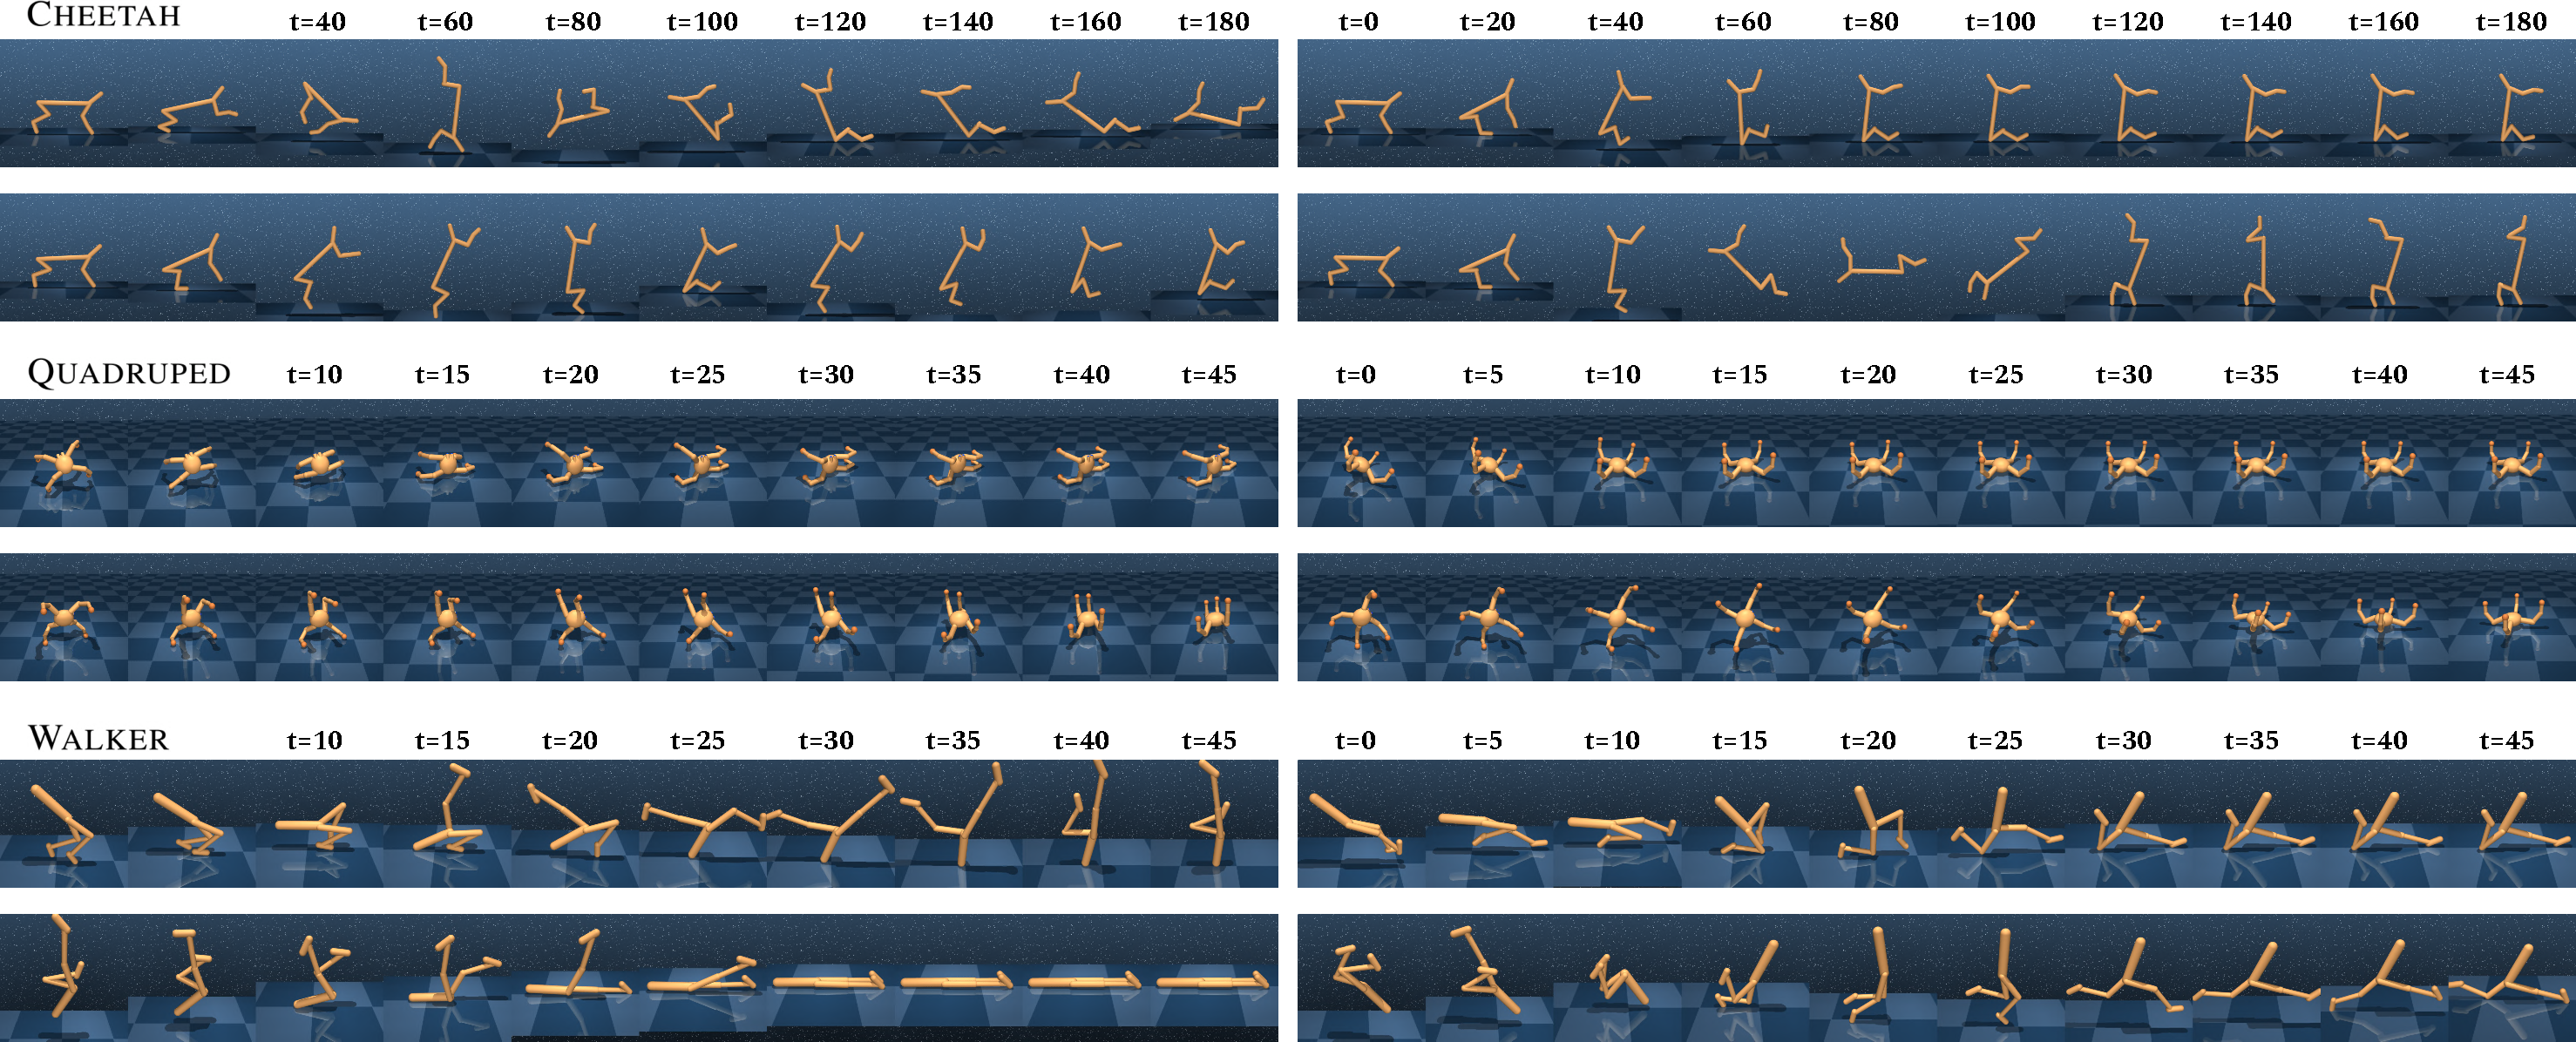
\includegraphics[width=\textwidth]{behaviors_more_compressed.pdf}}
\caption{Behaviors learned during pre-training on the \texttt{APS} dataset. Within each domain, behaviors correspond (clockwise) to $\mathbf{w}_{-\mathbf{e}_2}$, $\mathbf{w}_{+\mathbf{e}_2}$, $\mathbf{w}_{+\mathbf{e}_3}$, and $\mathbf{w}_{-\mathbf{e}_3}$.}
\label{fig:behaviors-appendix}
\end{figure*}



\section{Additional Results}

\subsection{Laplacian Behavior Basis}


Figure~\ref{fig:behaviors-appendix} visualizes additional behaviors induced by different weight vectors---specifically $\mathbf{w}_{-\mathbf{e}_2}$, $\mathbf{w}_{+\mathbf{e}_2}$, $\mathbf{w}_{-\mathbf{e}_3}$, and $\mathbf{w}_{+\mathbf{e}_3}$---across the three domains. For example, $\mathbf{w}_{-\mathbf{e}_2} = [0, -1, 0, \dots]$ induces a behavior that maximizes the negative of the second eigenvector.

We observe that the \textsc{Cheetah} exhibits behaviors such as backflipping, sitting on its hindquarters, hopping while seated, and transitioning from a backflip into a headstand. The \textsc{Quadruped} learns to lie on its side or back with distinct limb configurations, while the \textsc{Walker} acquires behaviors including headstands, multiple forms of splits, and lying flat on its back. While the specific behaviors discovered may vary across training runs and datasets due to stochasticity in the unsupervised optimization process, the approach consistently produces diverse and temporally coherent behaviors.







\begin{table}
\centering
\caption{Zero-shot performance comparison of FB and LK across datasets for $k=50$. Reported values are mean $\pm$ standard error, estimated from 30 independent runs.}
\label{tab:zero_shot_fb_lk_datasets}

\setlength{\tabcolsep}{10pt}
\renewcommand{\arraystretch}{1.2}

\footnotesize

\begin{tabular}{l r r r r r r}
\toprule
 & \multicolumn{2}{c}{\texttt{APS}} 
 & \multicolumn{2}{c}{\texttt{Proto}} 
 & \multicolumn{2}{c}{\texttt{RND}} \\
\cmidrule(lr){2-3} \cmidrule(lr){4-5} \cmidrule(lr){6-7}
\textbf{Task} 
& \multicolumn{1}{c}{FB} 
& \multicolumn{1}{c}{LK} 
& \multicolumn{1}{c}{FB} 
& \multicolumn{1}{c}{LK} 
& \multicolumn{1}{c}{FB} 
& \multicolumn{1}{c}{LK} \\
\midrule

\rowcolor{gray!15}
\textsc{Cheetah} \textit{(avg)} & 622 ${\scriptstyle \pm 31}$ & 591 ${\scriptstyle \pm 31}$ & 588 ${\scriptstyle \pm 33}$ & 551 ${\scriptstyle \pm 33}$ & 447 ${\scriptstyle \pm 27}$ & 208 ${\scriptstyle \pm 19}$ \\
\hspace{.5em} \texttt{Run} & 329 ${\scriptstyle \pm 17}$ & 265 ${\scriptstyle \pm 13}$ & 248 ${\scriptstyle \pm 8}$ & 216 ${\scriptstyle \pm 14}$ & 169 ${\scriptstyle \pm 9}$ & 108 ${\scriptstyle \pm 13}$ \\
\hspace{.5em} \texttt{Run-B} & 281 ${\scriptstyle \pm 8}$ & 297 ${\scriptstyle \pm 13}$ & 217 ${\scriptstyle \pm 8}$ & 217 ${\scriptstyle \pm 7}$ & 191 ${\scriptstyle \pm 9}$ & 51 ${\scriptstyle \pm 5}$ \\
\hspace{.5em} \texttt{Walk} & 899 ${\scriptstyle \pm 34}$ & 848 ${\scriptstyle \pm 30}$ & 937 ${\scriptstyle \pm 15}$ & 833 ${\scriptstyle \pm 38}$ & 621 ${\scriptstyle \pm 27}$ & 446 ${\scriptstyle \pm 43}$ \\
\hspace{.5em} \texttt{Walk-B} & 981 ${\scriptstyle \pm 3}$ & 953 ${\scriptstyle \pm 24}$ & 948 ${\scriptstyle \pm 14}$ & 937 ${\scriptstyle \pm 14}$ & 807 ${\scriptstyle \pm 27}$ & 228 ${\scriptstyle \pm 24}$ \\
\addlinespace
\rowcolor{gray!15}
\textsc{Quadruped} \textit{(avg)} & 612 ${\scriptstyle \pm 13}$ & 597 ${\scriptstyle \pm 17}$ & 228 ${\scriptstyle \pm 11}$ & 268 ${\scriptstyle \pm 12}$ & 569 ${\scriptstyle \pm 14}$ & 662 ${\scriptstyle \pm 17}$ \\
\hspace{.5em} \texttt{Jump} & 625 ${\scriptstyle \pm 12}$ & 674 ${\scriptstyle \pm 22}$ & 221 ${\scriptstyle \pm 15}$ & 288 ${\scriptstyle \pm 20}$ & 602 ${\scriptstyle \pm 8}$ & 701 ${\scriptstyle \pm 13}$ \\
\hspace{.5em} \texttt{Run} & 428 ${\scriptstyle \pm 10}$ & 425 ${\scriptstyle \pm 10}$ & 162 ${\scriptstyle \pm 13}$ & 204 ${\scriptstyle \pm 13}$ & 361 ${\scriptstyle \pm 7}$ & 470 ${\scriptstyle \pm 8}$ \\
\hspace{.5em} \texttt{Stand} & 799 ${\scriptstyle \pm 15}$ & 817 ${\scriptstyle \pm 23}$ & 332 ${\scriptstyle \pm 28}$ & 385 ${\scriptstyle \pm 28}$ & 720 ${\scriptstyle \pm 14}$ & 911 ${\scriptstyle \pm 14}$ \\
\hspace{.5em} \texttt{Walk} & 595 ${\scriptstyle \pm 12}$ & 470 ${\scriptstyle \pm 12}$ & 195 ${\scriptstyle \pm 13}$ & 195 ${\scriptstyle \pm 15}$ & 593 ${\scriptstyle \pm 22}$ & 565 ${\scriptstyle \pm 26}$ \\
\addlinespace
\rowcolor{gray!15}
\textsc{Walker} \textit{(avg)} & 484 ${\scriptstyle \pm 25}$ & 588 ${\scriptstyle \pm 22}$ & 665 ${\scriptstyle \pm 23}$ & 713 ${\scriptstyle \pm 24}$ & 604 ${\scriptstyle \pm 16}$ & 444 ${\scriptstyle \pm 29}$ \\
\hspace{.5em} \texttt{Flip} & 211 ${\scriptstyle \pm 20}$ & 604 ${\scriptstyle \pm 21}$ & 476 ${\scriptstyle \pm 30}$ & 682 ${\scriptstyle \pm 11}$ & 548 ${\scriptstyle \pm 19}$ & 236 ${\scriptstyle \pm 38}$ \\
\hspace{.5em} \texttt{Run} & 266 ${\scriptstyle \pm 16}$ & 327 ${\scriptstyle \pm 21}$ & 396 ${\scriptstyle \pm 13}$ & 343 ${\scriptstyle \pm 7}$ & 405 ${\scriptstyle \pm 7}$ & 211 ${\scriptstyle \pm 24}$ \\
\hspace{.5em} \texttt{Stand} & 660 ${\scriptstyle \pm 30}$ & 589 ${\scriptstyle \pm 45}$ & 896 ${\scriptstyle \pm 11}$ & 884 ${\scriptstyle \pm 37}$ & 704 ${\scriptstyle \pm 28}$ & 433 ${\scriptstyle \pm 33}$ \\
\hspace{.5em} \texttt{Walk} & 798 ${\scriptstyle \pm 15}$ & 833 ${\scriptstyle \pm 30}$ & 891 ${\scriptstyle \pm 8}$ & 941 ${\scriptstyle \pm 4}$ & 759 ${\scriptstyle \pm 14}$ & 896 ${\scriptstyle \pm 16}$ \\
\addlinespace

\bottomrule
\end{tabular}
\end{table}



\subsection{Generality of the Laplacian Basis}
\label{sec:generality-appx}

We report zero-shot performance of LK and FB with $k=50$ separately for each dataset in Table~\ref{tab:zero_shot_fb_lk_datasets}. The sign test is conducted using these dataset–task–specific results.
In Figure~\ref{fig:lk-lineplot-appendix}, we visualize zero-shot performance as a function of the basis size for each dataset separately, with the corresponding numerical values reported in Table~\ref{tab:lk_zero_shot_full_table}. While the qualitative trends relating performance to basis size discussed in the main paper largely persist, a closer inspection reveals dataset-specific structure. In particular, different datasets appear to preferentially benefit different domains.

For example, in \textsc{Cheetah}, performance is consistently higher when training on \texttt{APS} and \texttt{Proto} compared to \texttt{RND}, across all basis sizes. In contrast, for \textsc{Quadruped}, the highest performance is achieved when training on \texttt{RND}, indicating a clear dataset preference. Another pattern emerges in \texttt{Walker}: performance peaks at $k=20$ for most tasks when trained on \texttt{APS} and \texttt{Proto}, whereas it yields the lowest performance on \texttt{RND} across $k \in \{1, 2, 3, 5, 10, 20, 50\}$. These dataset-specific differences suggest that the quality of pretraining can induce approximation errors, highlighting the relevance of methods such as \citet{sikchi2025fast} for mitigating such effects.



\begin{figure*}
\centerline{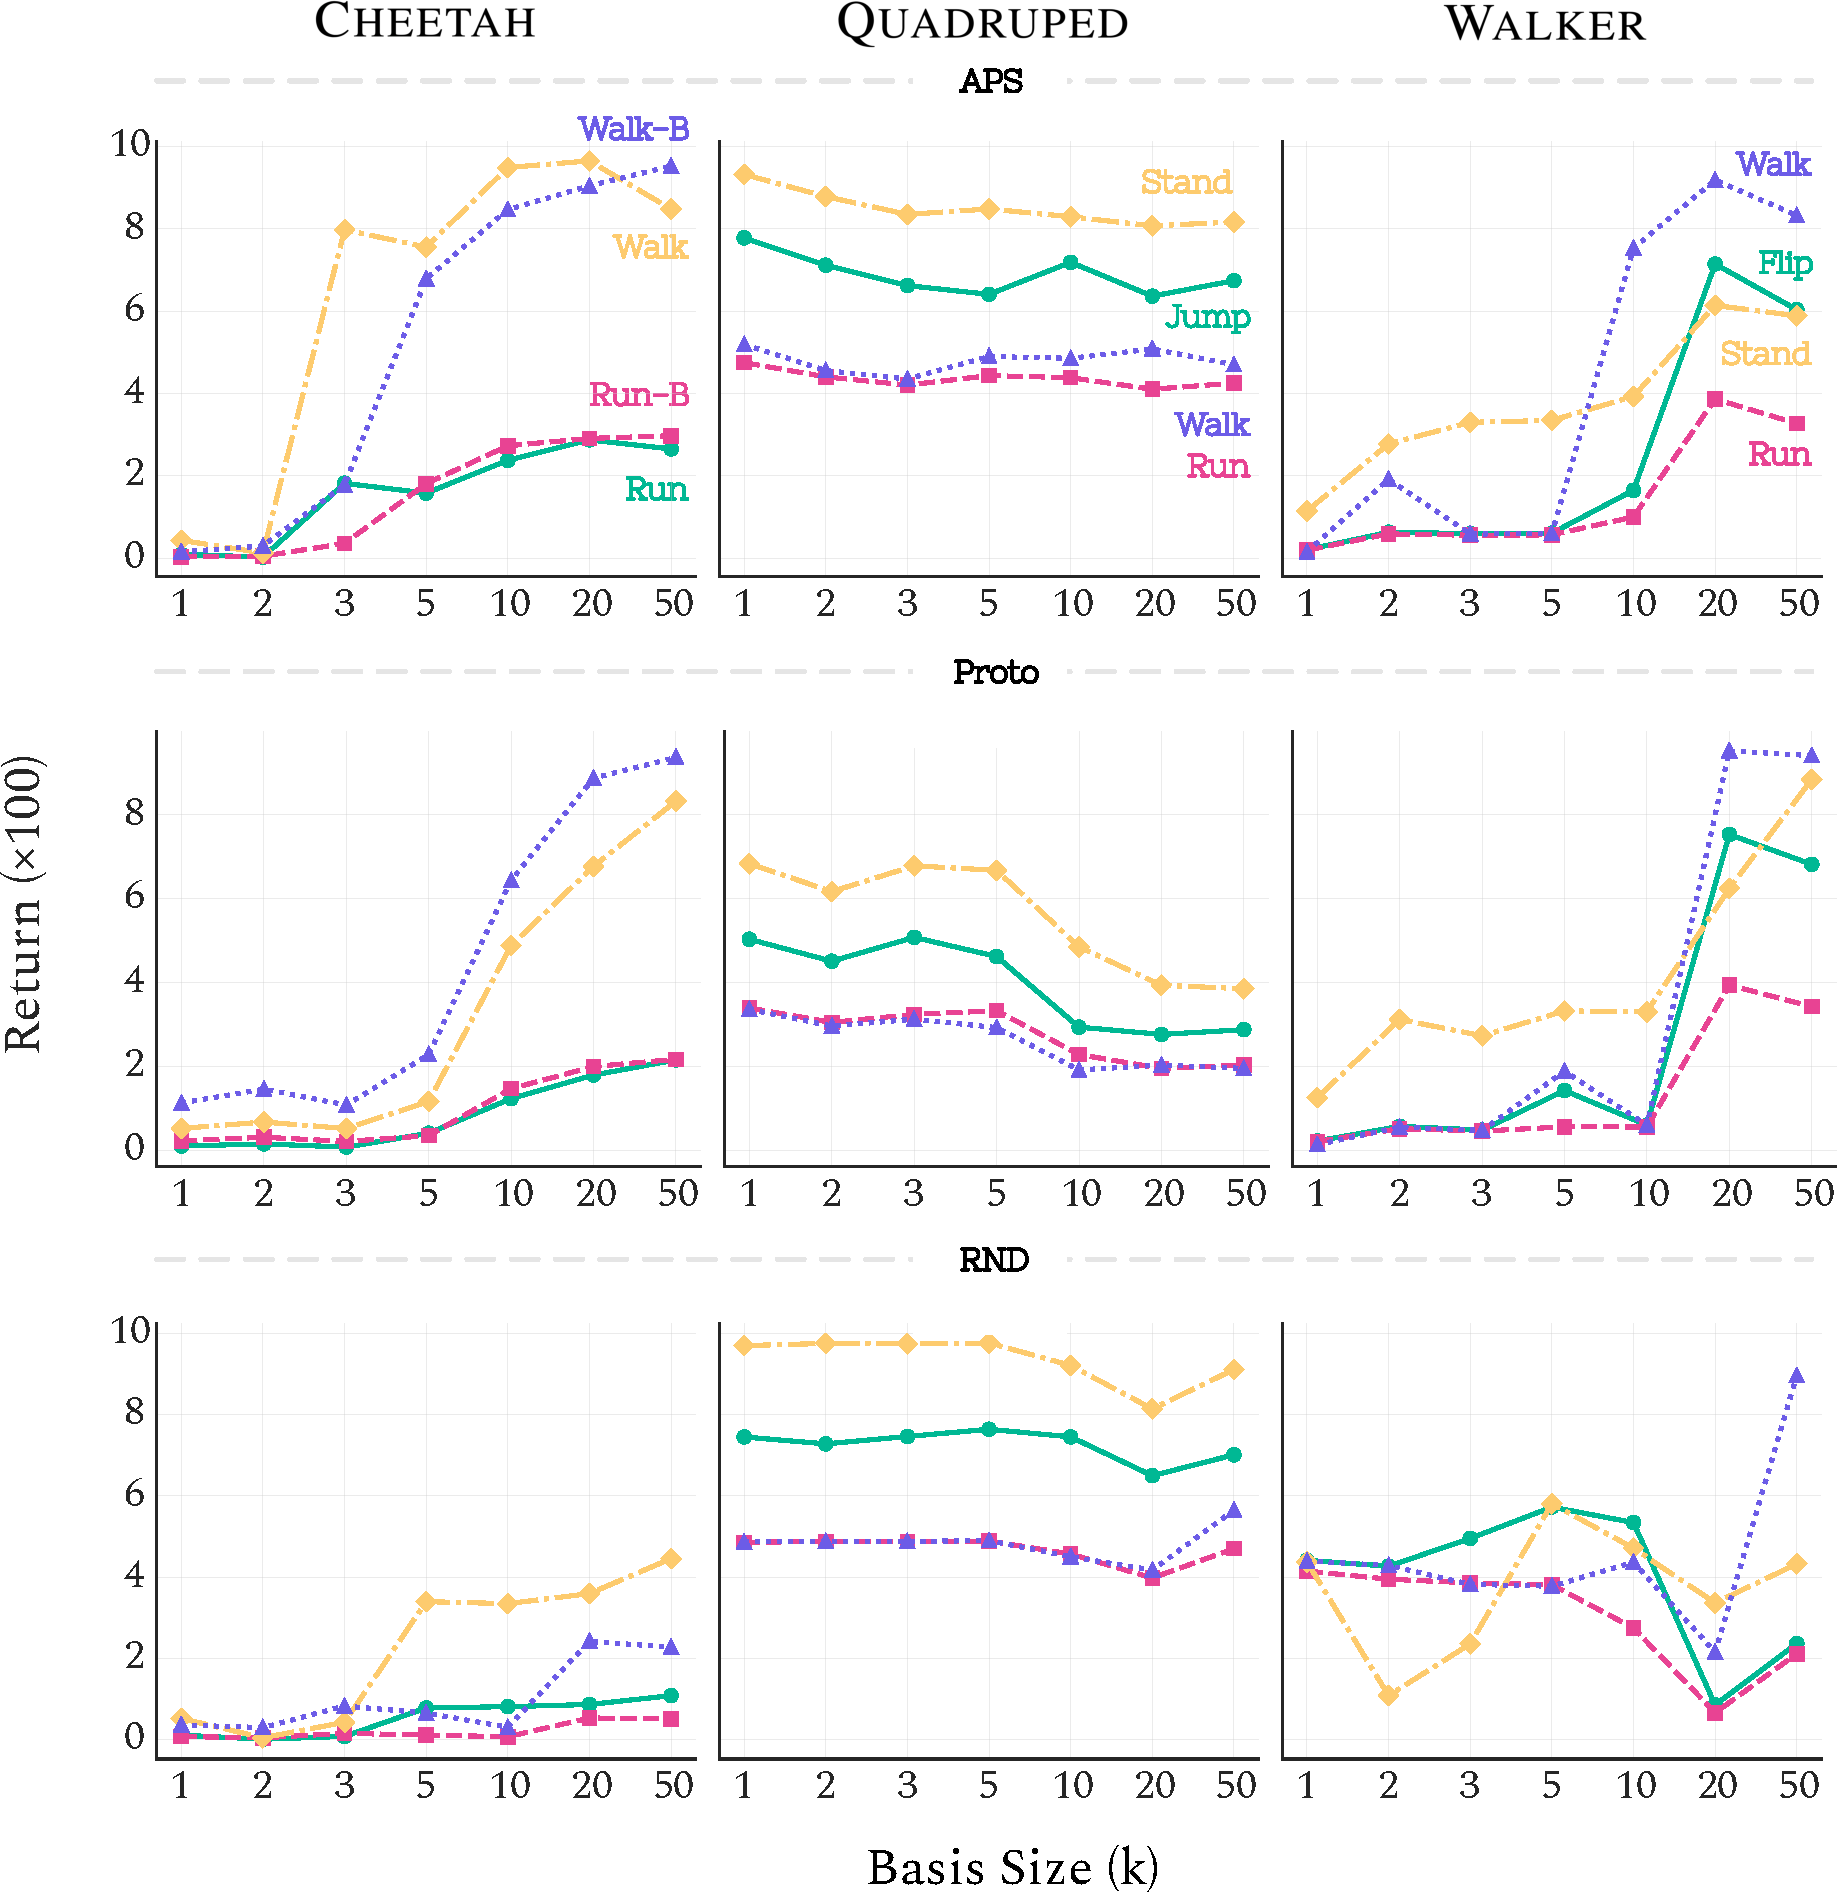
\includegraphics[width=.65\textwidth]{lk-lineplot-appendix.pdf}}
\caption{Zero-shot performance of LK as a function of basis size and dataset. Each row corresponds to a dataset, each curve to a task, and points indicate averages over 30 random seeds.}
\label{fig:lk-lineplot-appendix}
\end{figure*}


\begin{table}
\centering
\caption{Zero-shot performance of LK for different basis sizes and datasets. Reported values are mean $\pm$ standard error, estimated from 30 independent runs.}
\label{tab:lk_zero_shot_full_table}

\setlength{\tabcolsep}{7pt}
\renewcommand{\arraystretch}{1.2}

\footnotesize

\begin{tabular}{l l r r r r r r r}
\toprule
 & & \multicolumn{7}{c}{\textbf{Basis Size $k$}} \\
\cmidrule(lr){3-9}
\textbf{Dataset} & \textbf{Task}
& \multicolumn{1}{c}{1}
& \multicolumn{1}{c}{2}
& \multicolumn{1}{c}{3}
& \multicolumn{1}{c}{5}
& \multicolumn{1}{c}{10}
& \multicolumn{1}{c}{20}
& \multicolumn{1}{c}{50} \\
\midrule


 \rowcolor{gray!15}  \cellcolor{white} \texttt{APS} &  \domainavg{cheetah} & 17 ${\scriptstyle \pm 2}$ & 12 ${\scriptstyle \pm 3}$ & 298 ${\scriptstyle \pm 28}$ & 443 ${\scriptstyle \pm 29}$ & 577 ${\scriptstyle \pm 33}$ & 612 ${\scriptstyle \pm 32}$ & 591 ${\scriptstyle \pm 31}$ \\
& \hspace{.5em}\texttt{Run} & 9 ${\scriptstyle \pm 2}$ & 2 ${\scriptstyle \pm 0}$ & 182 ${\scriptstyle \pm 10}$ & 158 ${\scriptstyle \pm 6}$ & 238 ${\scriptstyle \pm 9}$ & 287 ${\scriptstyle \pm 10}$ & 265 ${\scriptstyle \pm 13}$ \\
& \hspace{.5em}\texttt{Run-B} & 3 ${\scriptstyle \pm 1}$ & 5 ${\scriptstyle \pm 2}$ & 36 ${\scriptstyle \pm 2}$ & 181 ${\scriptstyle \pm 12}$ & 273 ${\scriptstyle \pm 21}$ & 291 ${\scriptstyle \pm 19}$ & 297 ${\scriptstyle \pm 13}$ \\
& \hspace{.5em}\texttt{Walk} & 43 ${\scriptstyle \pm 7}$ & 12 ${\scriptstyle \pm 1}$ & 798 ${\scriptstyle \pm 32}$ & 756 ${\scriptstyle \pm 24}$ & 949 ${\scriptstyle \pm 8}$ & 965 ${\scriptstyle \pm 5}$ & 848 ${\scriptstyle \pm 30}$ \\
& \hspace{.5em}\texttt{Walk-B} & 15 ${\scriptstyle \pm 4}$ & 29 ${\scriptstyle \pm 12}$ & 178 ${\scriptstyle \pm 13}$ & 679 ${\scriptstyle \pm 48}$ & 847 ${\scriptstyle \pm 49}$ & 905 ${\scriptstyle \pm 39}$ & 953 ${\scriptstyle \pm 24}$ \\
\addlinespace
 \rowcolor{gray!15}  \cellcolor{white} & \domainavg{quadruped} & 676 ${\scriptstyle \pm 17}$ & 622 ${\scriptstyle \pm 17}$ & 588 ${\scriptstyle \pm 17}$ & 606 ${\scriptstyle \pm 16}$ & 618 ${\scriptstyle \pm 16}$ & 591 ${\scriptstyle \pm 16}$ & 597 ${\scriptstyle \pm 17}$ \\
& \hspace{.5em}\texttt{Jump} & 778 ${\scriptstyle \pm 5}$ & 712 ${\scriptstyle \pm 8}$ & 662 ${\scriptstyle \pm 9}$ & 641 ${\scriptstyle \pm 15}$ & 719 ${\scriptstyle \pm 12}$ & 637 ${\scriptstyle \pm 21}$ & 674 ${\scriptstyle \pm 22}$ \\
& \hspace{.5em}\texttt{Run} & 475 ${\scriptstyle \pm 1}$ & 440 ${\scriptstyle \pm 4}$ & 421 ${\scriptstyle \pm 5}$ & 443 ${\scriptstyle \pm 7}$ & 439 ${\scriptstyle \pm 6}$ & 410 ${\scriptstyle \pm 9}$ & 425 ${\scriptstyle \pm 10}$ \\
& \hspace{.5em}\texttt{Stand} & 933 ${\scriptstyle \pm 6}$ & 879 ${\scriptstyle \pm 9}$ & 835 ${\scriptstyle \pm 9}$ & 849 ${\scriptstyle \pm 15}$ & 830 ${\scriptstyle \pm 21}$ & 807 ${\scriptstyle \pm 20}$ & 817 ${\scriptstyle \pm 23}$ \\
& \hspace{.5em}\texttt{Walk} & 519 ${\scriptstyle \pm 7}$ & 456 ${\scriptstyle \pm 12}$ & 435 ${\scriptstyle \pm 18}$ & 490 ${\scriptstyle \pm 16}$ & 486 ${\scriptstyle \pm 9}$ & 508 ${\scriptstyle \pm 5}$ & 470 ${\scriptstyle \pm 12}$ \\
\addlinespace
 \rowcolor{gray!15}  \cellcolor{white} & \domainavg{walker} & 42 ${\scriptstyle \pm 4}$ & 148 ${\scriptstyle \pm 13}$ & 126 ${\scriptstyle \pm 11}$ & 128 ${\scriptstyle \pm 11}$ & 353 ${\scriptstyle \pm 30}$ & 659 ${\scriptstyle \pm 24}$ & 588 ${\scriptstyle \pm 22}$ \\
& \hspace{.5em}\texttt{Flip} & 20 ${\scriptstyle \pm 0}$ & 63 ${\scriptstyle \pm 1}$ & 60 ${\scriptstyle \pm 0}$ & 61 ${\scriptstyle \pm 0}$ & 165 ${\scriptstyle \pm 35}$ & 715 ${\scriptstyle \pm 26}$ & 604 ${\scriptstyle \pm 21}$ \\
& \hspace{.5em}\texttt{Run} & 19 ${\scriptstyle \pm 0}$ & 59 ${\scriptstyle \pm 1}$ & 56 ${\scriptstyle \pm 0}$ & 56 ${\scriptstyle \pm 0}$ & 100 ${\scriptstyle \pm 17}$ & 387 ${\scriptstyle \pm 18}$ & 327 ${\scriptstyle \pm 21}$ \\
& \hspace{.5em}\texttt{Stand} & 114 ${\scriptstyle \pm 2}$ & 277 ${\scriptstyle \pm 18}$ & 330 ${\scriptstyle \pm 0}$ & 335 ${\scriptstyle \pm 1}$ & 393 ${\scriptstyle \pm 27}$ & 614 ${\scriptstyle \pm 56}$ & 589 ${\scriptstyle \pm 45}$ \\
& \hspace{.5em}\texttt{Walk} & 15 ${\scriptstyle \pm 1}$ & 192 ${\scriptstyle \pm 37}$ & 59 ${\scriptstyle \pm 0}$ & 60 ${\scriptstyle \pm 0}$ & 753 ${\scriptstyle \pm 61}$ & 919 ${\scriptstyle \pm 20}$ & 833 ${\scriptstyle \pm 30}$ \\
\addlinespace
\midrule
 \rowcolor{gray!15}  \cellcolor{white}\texttt{Proto} & \domainavg{cheetah} & 50 ${\scriptstyle \pm 6}$ & 65 ${\scriptstyle \pm 10}$ & 47 ${\scriptstyle \pm 7}$ & 105 ${\scriptstyle \pm 17}$ & 351 ${\scriptstyle \pm 31}$ & 486 ${\scriptstyle \pm 32}$ & 551 ${\scriptstyle \pm 33}$ \\
& \hspace{.5em}\texttt{Run} & 10 ${\scriptstyle \pm 1}$ & 15 ${\scriptstyle \pm 5}$ & 8 ${\scriptstyle \pm 1}$ & 41 ${\scriptstyle \pm 9}$ & 123 ${\scriptstyle \pm 16}$ & 180 ${\scriptstyle \pm 14}$ & 216 ${\scriptstyle \pm 14}$ \\
& \hspace{.5em}\texttt{Run-B} & 23 ${\scriptstyle \pm 3}$ & 31 ${\scriptstyle \pm 4}$ & 21 ${\scriptstyle \pm 4}$ & 35 ${\scriptstyle \pm 9}$ & 147 ${\scriptstyle \pm 15}$ & 200 ${\scriptstyle \pm 10}$ & 217 ${\scriptstyle \pm 7}$ \\
& \hspace{.5em}\texttt{Walk} & 52 ${\scriptstyle \pm 6}$ & 67 ${\scriptstyle \pm 25}$ & 52 ${\scriptstyle \pm 11}$ & 117 ${\scriptstyle \pm 30}$ & 488 ${\scriptstyle \pm 65}$ & 677 ${\scriptstyle \pm 61}$ & 833 ${\scriptstyle \pm 38}$ \\
& \hspace{.5em}\texttt{Walk-B} & 113 ${\scriptstyle \pm 16}$ & 146 ${\scriptstyle \pm 22}$ & 108 ${\scriptstyle \pm 20}$ & 228 ${\scriptstyle \pm 53}$ & 644 ${\scriptstyle \pm 63}$ & 888 ${\scriptstyle \pm 21}$ & 937 ${\scriptstyle \pm 14}$ \\
\addlinespace
 \rowcolor{gray!15}  \cellcolor{white} & \domainavg{quadruped} & 466 ${\scriptstyle \pm 16}$ & 417 ${\scriptstyle \pm 17}$ & 456 ${\scriptstyle \pm 18}$ & 439 ${\scriptstyle \pm 19}$ & 300 ${\scriptstyle \pm 15}$ & 267 ${\scriptstyle \pm 14}$ & 268 ${\scriptstyle \pm 12}$ \\
& \hspace{.5em}\texttt{Jump} & 503 ${\scriptstyle \pm 18}$ & 451 ${\scriptstyle \pm 21}$ & 508 ${\scriptstyle \pm 24}$ & 462 ${\scriptstyle \pm 30}$ & 294 ${\scriptstyle \pm 22}$ & 276 ${\scriptstyle \pm 23}$ & 288 ${\scriptstyle \pm 20}$ \\
& \hspace{.5em}\texttt{Run} & 339 ${\scriptstyle \pm 14}$ & 305 ${\scriptstyle \pm 18}$ & 324 ${\scriptstyle \pm 17}$ & 333 ${\scriptstyle \pm 18}$ & 228 ${\scriptstyle \pm 16}$ & 195 ${\scriptstyle \pm 15}$ & 204 ${\scriptstyle \pm 13}$ \\
& \hspace{.5em}\texttt{Stand} & 684 ${\scriptstyle \pm 27}$ & 617 ${\scriptstyle \pm 34}$ & 679 ${\scriptstyle \pm 33}$ & 668 ${\scriptstyle \pm 36}$ & 485 ${\scriptstyle \pm 33}$ & 394 ${\scriptstyle \pm 36}$ & 385 ${\scriptstyle \pm 28}$ \\
& \hspace{.5em}\texttt{Walk} & 336 ${\scriptstyle \pm 16}$ & 296 ${\scriptstyle \pm 20}$ & 313 ${\scriptstyle \pm 18}$ & 293 ${\scriptstyle \pm 23}$ & 192 ${\scriptstyle \pm 14}$ & 204 ${\scriptstyle \pm 18}$ & 195 ${\scriptstyle \pm 15}$ \\
\addlinespace
  \rowcolor{gray!15}  \cellcolor{white} & \domainavg{walker} & 46 ${\scriptstyle \pm 4}$ & 119 ${\scriptstyle \pm 10}$ & 104 ${\scriptstyle \pm 9}$ & 180 ${\scriptstyle \pm 19}$ & 127 ${\scriptstyle \pm 11}$ & 681 ${\scriptstyle \pm 24}$ & 713 ${\scriptstyle \pm 24}$ \\
& \hspace{.5em}\texttt{Flip} & 22 ${\scriptstyle \pm 1}$ & 57 ${\scriptstyle \pm 2}$ & 48 ${\scriptstyle \pm 2}$ & 142 ${\scriptstyle \pm 38}$ & 60 ${\scriptstyle \pm 0}$ & 753 ${\scriptstyle \pm 25}$ & 682 ${\scriptstyle \pm 11}$ \\
& \hspace{.5em}\texttt{Run} & 21 ${\scriptstyle \pm 1}$ & 52 ${\scriptstyle \pm 1}$ & 46 ${\scriptstyle \pm 2}$ & 56 ${\scriptstyle \pm 0}$ & 56 ${\scriptstyle \pm 0}$ & 394 ${\scriptstyle \pm 9}$ & 343 ${\scriptstyle \pm 7}$ \\
& \hspace{.5em}\texttt{Stand} & 126 ${\scriptstyle \pm 6}$ & 312 ${\scriptstyle \pm 9}$ & 273 ${\scriptstyle \pm 12}$ & 333 ${\scriptstyle \pm 1}$ & 330 ${\scriptstyle \pm 1}$ & 625 ${\scriptstyle \pm 54}$ & 884 ${\scriptstyle \pm 37}$ \\
& \hspace{.5em}\texttt{Walk} & 14 ${\scriptstyle \pm 1}$ & 56 ${\scriptstyle \pm 2}$ & 47 ${\scriptstyle \pm 2}$ & 189 ${\scriptstyle \pm 55}$ & 60 ${\scriptstyle \pm 0}$ & 953 ${\scriptstyle \pm 2}$ & 941 ${\scriptstyle \pm 4}$ \\
\addlinespace
\midrule
 \rowcolor{gray!15}  \cellcolor{white} \texttt{RND} & \domainavg{cheetah} & 26 ${\scriptstyle \pm 3}$ & 10 ${\scriptstyle \pm 1}$ & 37 ${\scriptstyle \pm 5}$ & 123 ${\scriptstyle \pm 15}$ & 113 ${\scriptstyle \pm 13}$ & 185 ${\scriptstyle \pm 13}$ & 208 ${\scriptstyle \pm 19}$ \\
& \hspace{.5em}\texttt{Run} & 11 ${\scriptstyle \pm 2}$ & 1 ${\scriptstyle \pm 0}$ & 8 ${\scriptstyle \pm 2}$ & 78 ${\scriptstyle \pm 8}$ & 81 ${\scriptstyle \pm 6}$ & 86 ${\scriptstyle \pm 3}$ & 108 ${\scriptstyle \pm 13}$ \\
& \hspace{.5em}\texttt{Run-B} & 7 ${\scriptstyle \pm 1}$ & 4 ${\scriptstyle \pm 1}$ & 15 ${\scriptstyle \pm 3}$ & 11 ${\scriptstyle \pm 2}$ & 7 ${\scriptstyle \pm 1}$ & 53 ${\scriptstyle \pm 4}$ & 51 ${\scriptstyle \pm 5}$ \\
& \hspace{.5em}\texttt{Walk} & 52 ${\scriptstyle \pm 9}$ & 4 ${\scriptstyle \pm 1}$ & 43 ${\scriptstyle \pm 10}$ & 340 ${\scriptstyle \pm 32}$ & 335 ${\scriptstyle \pm 21}$ & 359 ${\scriptstyle \pm 14}$ & 446 ${\scriptstyle \pm 43}$ \\
& \hspace{.5em}\texttt{Walk-B} & 36 ${\scriptstyle \pm 5}$ & 29 ${\scriptstyle \pm 4}$ & 82 ${\scriptstyle \pm 15}$ & 65 ${\scriptstyle \pm 13}$ & 30 ${\scriptstyle \pm 6}$ & 242 ${\scriptstyle \pm 22}$ & 228 ${\scriptstyle \pm 24}$ \\
\addlinespace
 \rowcolor{gray!15}  \cellcolor{white} & \domainavg{quadruped} & 672 ${\scriptstyle \pm 19}$ & 670 ${\scriptstyle \pm 19}$ & 674 ${\scriptstyle \pm 19}$ & 680 ${\scriptstyle \pm 19}$ & 644 ${\scriptstyle \pm 19}$ & 570 ${\scriptstyle \pm 19}$ & 662 ${\scriptstyle \pm 17}$ \\
& \hspace{.5em}\texttt{Jump} & 745 ${\scriptstyle \pm 11}$ & 728 ${\scriptstyle \pm 7}$ & 746 ${\scriptstyle \pm 9}$ & 764 ${\scriptstyle \pm 6}$ & 746 ${\scriptstyle \pm 12}$ & 650 ${\scriptstyle \pm 22}$ & 701 ${\scriptstyle \pm 13}$ \\
& \hspace{.5em}\texttt{Run} & 486 ${\scriptstyle \pm 2}$ & 488 ${\scriptstyle \pm 1}$ & 488 ${\scriptstyle \pm 1}$ & 489 ${\scriptstyle \pm 0}$ & 457 ${\scriptstyle \pm 10}$ & 398 ${\scriptstyle \pm 14}$ & 470 ${\scriptstyle \pm 8}$ \\
& \hspace{.5em}\texttt{Stand} & 970 ${\scriptstyle \pm 3}$ & 976 ${\scriptstyle \pm 1}$ & 975 ${\scriptstyle \pm 1}$ & 977 ${\scriptstyle \pm 1}$ & 922 ${\scriptstyle \pm 18}$ & 815 ${\scriptstyle \pm 28}$ & 911 ${\scriptstyle \pm 14}$ \\
& \hspace{.5em}\texttt{Walk} & 487 ${\scriptstyle \pm 3}$ & 488 ${\scriptstyle \pm 2}$ & 488 ${\scriptstyle \pm 3}$ & 490 ${\scriptstyle \pm 2}$ & 450 ${\scriptstyle \pm 10}$ & 417 ${\scriptstyle \pm 18}$ & 565 ${\scriptstyle \pm 26}$ \\
\addlinespace
 \rowcolor{gray!15}  \cellcolor{white} & \domainavg{walker} & 433 ${\scriptstyle \pm 2}$ & 340 ${\scriptstyle \pm 12}$ & 375 ${\scriptstyle \pm 12}$ & 478 ${\scriptstyle \pm 9}$ & 429 ${\scriptstyle \pm 14}$ & 176 ${\scriptstyle \pm 17}$ & 444 ${\scriptstyle \pm 29}$ \\
& \hspace{.5em}\texttt{Flip} & 441 ${\scriptstyle \pm 2}$ & 427 ${\scriptstyle \pm 2}$ & 495 ${\scriptstyle \pm 10}$ & 573 ${\scriptstyle \pm 2}$ & 534 ${\scriptstyle \pm 17}$ & 85 ${\scriptstyle \pm 6}$ & 236 ${\scriptstyle \pm 38}$ \\
& \hspace{.5em}\texttt{Run} & 415 ${\scriptstyle \pm 3}$ & 395 ${\scriptstyle \pm 3}$ & 386 ${\scriptstyle \pm 4}$ & 381 ${\scriptstyle \pm 3}$ & 275 ${\scriptstyle \pm 14}$ & 66 ${\scriptstyle \pm 7}$ & 211 ${\scriptstyle \pm 24}$ \\
& \hspace{.5em}\texttt{Stand} & 438 ${\scriptstyle \pm 4}$ & 108 ${\scriptstyle \pm 1}$ & 236 ${\scriptstyle \pm 31}$ & 581 ${\scriptstyle \pm 2}$ & 472 ${\scriptstyle \pm 35}$ & 337 ${\scriptstyle \pm 3}$ & 433 ${\scriptstyle \pm 33}$ \\
& \hspace{.5em}\texttt{Walk} & 440 ${\scriptstyle \pm 2}$ & 429 ${\scriptstyle \pm 2}$ & 382 ${\scriptstyle \pm 7}$ & 378 ${\scriptstyle \pm 8}$ & 437 ${\scriptstyle \pm 11}$ & 215 ${\scriptstyle \pm 53}$ & 896 ${\scriptstyle \pm 16}$ \\
\addlinespace

\bottomrule

\end{tabular}
\end{table}


\newpage
\subsection{Hierarchical Composition}
\label{sec:hier-comp-appendix}

\begin{table}[H]
\centering
\caption{Relative percentage improvement of LK over its zero-shot baseline for varying basis sizes. Reported values are mean $\pm$ standard error, estimated from 30 independent runs.}
\label{tab:perc_imp_fb_lk_appendix}

\setlength{\tabcolsep}{5pt}
\renewcommand{\arraystretch}{1.1}
\footnotesize

\begin{tabular}{l l r r r r r r r}
\toprule
 & & \multicolumn{7}{c}{\textbf{Improvement (\%) for Basis Size $k$}} \\
\cmidrule(lr){3-9}
\textbf{Dataset} & \textbf{Task}
& \multicolumn{1}{c}{1}
& \multicolumn{1}{c}{2}
& \multicolumn{1}{c}{3}
& \multicolumn{1}{c}{5}
& \multicolumn{1}{c}{10}
& \multicolumn{1}{c}{20}
& \multicolumn{1}{c}{50} \\
\midrule

 \rowcolor{gray!15}  \cellcolor{white} \texttt{APS} &\domainavg{cheetah} & 14701 ${\scriptstyle \pm 3418}$ & 11496 ${\scriptstyle \pm 2909}$ & 219 ${\scriptstyle \pm 28}$ & 98 ${\scriptstyle \pm 103}$ & 15 ${\scriptstyle \pm 9}$ & -3 ${\scriptstyle \pm 5}$ & 0 ${\scriptstyle \pm 6}$ \\
& \hspace{.5em} \texttt{Run} & 9143 ${\scriptstyle \pm 4069}$ & 5474 ${\scriptstyle \pm 705}$ & 34 ${\scriptstyle \pm 9}$ & -21 ${\scriptstyle \pm 11}$ & 17 ${\scriptstyle \pm 7}$ & 15 ${\scriptstyle \pm 5}$ & 20 ${\scriptstyle \pm 9}$ \\
& \hspace{.5em} \texttt{Run-B} & 25129 ${\scriptstyle \pm 9453}$ & 21084 ${\scriptstyle \pm 9546}$ & 497 ${\scriptstyle \pm 69}$ & 16 ${\scriptstyle \pm 11}$ & 31 ${\scriptstyle \pm 30}$ & -22 ${\scriptstyle \pm 14}$ & -6 ${\scriptstyle \pm 22}$ \\
& \hspace{.5em} \texttt{Walk} & 1956 ${\scriptstyle \pm 487}$ & 4169 ${\scriptstyle \pm 531}$ & 20 ${\scriptstyle \pm 6}$ & -25 ${\scriptstyle \pm 7}$ & -7 ${\scriptstyle \pm 4}$ & -2 ${\scriptstyle \pm 1}$ & 7 ${\scriptstyle \pm 7}$ \\
& \hspace{.5em} \texttt{Walk-B} & 22575 ${\scriptstyle \pm 8544}$ & 15258 ${\scriptstyle \pm 6347}$ & 325 ${\scriptstyle \pm 50}$ & 424 ${\scriptstyle \pm 411}$ & 20 ${\scriptstyle \pm 15}$ & -4 ${\scriptstyle \pm 12}$ & -20 ${\scriptstyle \pm 6}$ \\
\addlinespace
 \rowcolor{gray!15}  \cellcolor{white} & \domainavg{quadruped} & 0 ${\scriptstyle \pm 0}$ & -11 ${\scriptstyle \pm 2}$ & -8 ${\scriptstyle \pm 3}$ & 4 ${\scriptstyle \pm 2}$ & 3 ${\scriptstyle \pm 3}$ & 23 ${\scriptstyle \pm 2}$ & 26 ${\scriptstyle \pm 3}$ \\
& \hspace{.5em} \texttt{Jump} & 0 ${\scriptstyle \pm 0}$ & -18 ${\scriptstyle \pm 5}$ & -15 ${\scriptstyle \pm 4}$ & 4 ${\scriptstyle \pm 4}$ & -15 ${\scriptstyle \pm 3}$ & 21 ${\scriptstyle \pm 6}$ & 16 ${\scriptstyle \pm 5}$ \\
& \hspace{.5em} \texttt{Run} & 0 ${\scriptstyle \pm 0}$ & -11 ${\scriptstyle \pm 4}$ & -10 ${\scriptstyle \pm 4}$ & 1 ${\scriptstyle \pm 2}$ & 2 ${\scriptstyle \pm 2}$ & 20 ${\scriptstyle \pm 3}$ & 14 ${\scriptstyle \pm 4}$ \\
& \hspace{.5em} \texttt{Stand} & 0 ${\scriptstyle \pm 0}$ & -21 ${\scriptstyle \pm 3}$ & -15 ${\scriptstyle \pm 4}$ & -4 ${\scriptstyle \pm 3}$ & -1 ${\scriptstyle \pm 4}$ & 17 ${\scriptstyle \pm 3}$ & 15 ${\scriptstyle \pm 4}$ \\
& \hspace{.5em} \texttt{Walk} & 1 ${\scriptstyle \pm 0}$ & 6 ${\scriptstyle \pm 5}$ & 9 ${\scriptstyle \pm 8}$ & 18 ${\scriptstyle \pm 7}$ & 25 ${\scriptstyle \pm 7}$ & 34 ${\scriptstyle \pm 3}$ & 59 ${\scriptstyle \pm 5}$ \\
\addlinespace
 \rowcolor{gray!15}  \cellcolor{white} & \domainavg{walker} & 1399 ${\scriptstyle \pm 117}$ & 341 ${\scriptstyle \pm 22}$ & 393 ${\scriptstyle \pm 25}$ & 444 ${\scriptstyle \pm 27}$ & 447 ${\scriptstyle \pm 44}$ & 59 ${\scriptstyle \pm 14}$ & 72 ${\scriptstyle \pm 18}$ \\
& \hspace{.5em} \texttt{Flip} & 1299 ${\scriptstyle \pm 18}$ & 451 ${\scriptstyle \pm 22}$ & 492 ${\scriptstyle \pm 11}$ & 556 ${\scriptstyle \pm 12}$ & 894 ${\scriptstyle \pm 96}$ & 54 ${\scriptstyle \pm 37}$ & 52 ${\scriptstyle \pm 36}$ \\
& \hspace{.5em} \texttt{Run} & 682 ${\scriptstyle \pm 10}$ & 254 ${\scriptstyle \pm 16}$ & 217 ${\scriptstyle \pm 6}$ & 255 ${\scriptstyle \pm 9}$ & 504 ${\scriptstyle \pm 42}$ & 73 ${\scriptstyle \pm 37}$ & 92 ${\scriptstyle \pm 35}$ \\
& \hspace{.5em} \texttt{Stand} & 378 ${\scriptstyle \pm 7}$ & 172 ${\scriptstyle \pm 25}$ & 88 ${\scriptstyle \pm 4}$ & 102 ${\scriptstyle \pm 5}$ & 157 ${\scriptstyle \pm 10}$ & 101 ${\scriptstyle \pm 17}$ & 86 ${\scriptstyle \pm 14}$ \\
& \hspace{.5em} \texttt{Walk} & 3237 ${\scriptstyle \pm 229}$ & 488 ${\scriptstyle \pm 64}$ & 774 ${\scriptstyle \pm 13}$ & 863 ${\scriptstyle \pm 17}$ & 234 ${\scriptstyle \pm 96}$ & 6 ${\scriptstyle \pm 4}$ & 60 ${\scriptstyle \pm 51}$ \\
\addlinespace
\midrule
 \rowcolor{gray!15}  \cellcolor{white} \texttt{Proto} & \domainavg{cheetah} & 1987 ${\scriptstyle \pm 562}$ & 8217 ${\scriptstyle \pm 2506}$ & 7672 ${\scriptstyle \pm 1416}$ & 21718 ${\scriptstyle \pm 11966}$ & 931 ${\scriptstyle \pm 432}$ & 148 ${\scriptstyle \pm 69}$ & 39 ${\scriptstyle \pm 16}$ \\
& \hspace{.5em} \texttt{Run} & 2137 ${\scriptstyle \pm 762}$ & 15471 ${\scriptstyle \pm 6801}$ & 14704 ${\scriptstyle \pm 4255}$ & 63998 ${\scriptstyle \pm 47246}$ & 531 ${\scriptstyle \pm 201}$ & 141 ${\scriptstyle \pm 41}$ & 99 ${\scriptstyle \pm 61}$ \\
& \hspace{.5em} \texttt{Run-B} & 2137 ${\scriptstyle \pm 1420}$ & 2517 ${\scriptstyle \pm 1302}$ & 3799 ${\scriptstyle \pm 1381}$ & 7625 ${\scriptstyle \pm 2111}$ & 1804 ${\scriptstyle \pm 1611}$ & 38 ${\scriptstyle \pm 10}$ & 26 ${\scriptstyle \pm 5}$ \\
& \hspace{.5em} \texttt{Walk} & 1626 ${\scriptstyle \pm 750}$ & 13815 ${\scriptstyle \pm 7010}$ & 6496 ${\scriptstyle \pm 1692}$ & 9069 ${\scriptstyle \pm 5209}$ & 571 ${\scriptstyle \pm 229}$ & 403 ${\scriptstyle \pm 268}$ & 29 ${\scriptstyle \pm 14}$ \\
& \hspace{.5em} \texttt{Walk-B} & 2048 ${\scriptstyle \pm 1418}$ & 1066 ${\scriptstyle \pm 459}$ & 5690 ${\scriptstyle \pm 2763}$ & 6180 ${\scriptstyle \pm 2084}$ & 818 ${\scriptstyle \pm 580}$ & 10 ${\scriptstyle \pm 4}$ & 2 ${\scriptstyle \pm 2}$ \\
\addlinespace
 \rowcolor{gray!15}  \cellcolor{white} & \domainavg{quadruped} & -10 ${\scriptstyle \pm 3}$ & -22 ${\scriptstyle \pm 4}$ & -5 ${\scriptstyle \pm 5}$ & -28 ${\scriptstyle \pm 7}$ & 1 ${\scriptstyle \pm 6}$ & 42 ${\scriptstyle \pm 9}$ & -2 ${\scriptstyle \pm 7}$ \\
& \hspace{.5em} \texttt{Jump} & -9 ${\scriptstyle \pm 6}$ & -14 ${\scriptstyle \pm 7}$ & -19 ${\scriptstyle \pm 6}$ & -40 ${\scriptstyle \pm 11}$ & 1 ${\scriptstyle \pm 14}$ & 37 ${\scriptstyle \pm 17}$ & -5 ${\scriptstyle \pm 10}$ \\
& \hspace{.5em} \texttt{Run} & -15 ${\scriptstyle \pm 7}$ & -19 ${\scriptstyle \pm 9}$ & -7 ${\scriptstyle \pm 9}$ & -44 ${\scriptstyle \pm 6}$ & -10 ${\scriptstyle \pm 8}$ & 33 ${\scriptstyle \pm 13}$ & -1 ${\scriptstyle \pm 15}$ \\
& \hspace{.5em} \texttt{Stand} & 2 ${\scriptstyle \pm 2}$ & -26 ${\scriptstyle \pm 7}$ & -7 ${\scriptstyle \pm 10}$ & -26 ${\scriptstyle \pm 8}$ & -11 ${\scriptstyle \pm 8}$ & 37 ${\scriptstyle \pm 16}$ & 14 ${\scriptstyle \pm 14}$ \\
& \hspace{.5em} \texttt{Walk} & -19 ${\scriptstyle \pm 7}$ & -28 ${\scriptstyle \pm 10}$ & 12 ${\scriptstyle \pm 12}$ & -3 ${\scriptstyle \pm 21}$ & 24 ${\scriptstyle \pm 16}$ & 60 ${\scriptstyle \pm 24}$ & -14 ${\scriptstyle \pm 18}$ \\
\addlinespace
 \rowcolor{gray!15}  \cellcolor{white} & \domainavg{walker} & 1264 ${\scriptstyle \pm 102}$ & 388 ${\scriptstyle \pm 26}$ & 549 ${\scriptstyle \pm 40}$ & 623 ${\scriptstyle \pm 39}$ & 799 ${\scriptstyle \pm 41}$ & 41 ${\scriptstyle \pm 11}$ & 9 ${\scriptstyle \pm 3}$ \\
& \hspace{.5em} \texttt{Flip} & 1168 ${\scriptstyle \pm 42}$ & 467 ${\scriptstyle \pm 25}$ & 690 ${\scriptstyle \pm 63}$ & 790 ${\scriptstyle \pm 59}$ & 997 ${\scriptstyle \pm 18}$ & 49 ${\scriptstyle \pm 38}$ & 10 ${\scriptstyle \pm 2}$ \\
& \hspace{.5em} \texttt{Run} & 583 ${\scriptstyle \pm 23}$ & 223 ${\scriptstyle \pm 10}$ & 309 ${\scriptstyle \pm 26}$ & 534 ${\scriptstyle \pm 8}$ & 660 ${\scriptstyle \pm 12}$ & 23 ${\scriptstyle \pm 5}$ & 19 ${\scriptstyle \pm 3}$ \\
& \hspace{.5em} \texttt{Stand} & 324 ${\scriptstyle \pm 13}$ & 85 ${\scriptstyle \pm 7}$ & 141 ${\scriptstyle \pm 14}$ & 157 ${\scriptstyle \pm 3}$ & 172 ${\scriptstyle \pm 1}$ & 94 ${\scriptstyle \pm 16}$ & 13 ${\scriptstyle \pm 10}$ \\
& \hspace{.5em} \texttt{Walk} & 2979 ${\scriptstyle \pm 141}$ & 778 ${\scriptstyle \pm 30}$ & 1056 ${\scriptstyle \pm 66}$ & 1009 ${\scriptstyle \pm 84}$ & 1365 ${\scriptstyle \pm 9}$ & -1 ${\scriptstyle \pm 0}$ & -4 ${\scriptstyle \pm 1}$ \\
\addlinespace
\midrule
 \rowcolor{gray!15}  \cellcolor{white} \texttt{RND} & \domainavg{cheetah} & 4500 ${\scriptstyle \pm 829}$ & 18658 ${\scriptstyle \pm 5725}$ & 11940 ${\scriptstyle \pm 5242}$ & 909 ${\scriptstyle \pm 162}$ & 1137 ${\scriptstyle \pm 178}$ & 111 ${\scriptstyle \pm 24}$ & 335 ${\scriptstyle \pm 164}$ \\
& \hspace{.5em} \texttt{Run} & 3985 ${\scriptstyle \pm 1491}$ & 37205 ${\scriptstyle \pm 18305}$ & 14968 ${\scriptstyle \pm 5701}$ & 182 ${\scriptstyle \pm 40}$ & 77 ${\scriptstyle \pm 14}$ & 78 ${\scriptstyle \pm 17}$ & 907 ${\scriptstyle \pm 637}$ \\
& \hspace{.5em} \texttt{Run-B} & 4743 ${\scriptstyle \pm 1472}$ & 4936 ${\scriptstyle \pm 1341}$ & 1800 ${\scriptstyle \pm 655}$ & 2049 ${\scriptstyle \pm 522}$ & 2331 ${\scriptstyle \pm 531}$ & 148 ${\scriptstyle \pm 59}$ & 137 ${\scriptstyle \pm 76}$ \\
& \hspace{.5em} \texttt{Walk} & 4443 ${\scriptstyle \pm 2132}$ & 29938 ${\scriptstyle \pm 13003}$ & 29536 ${\scriptstyle \pm 19978}$ & 103 ${\scriptstyle \pm 29}$ & 69 ${\scriptstyle \pm 11}$ & 41 ${\scriptstyle \pm 11}$ & 177 ${\scriptstyle \pm 104}$ \\
& \hspace{.5em} \texttt{Walk-B} & 4829 ${\scriptstyle \pm 1527}$ & 2556 ${\scriptstyle \pm 644}$ & 1457 ${\scriptstyle \pm 816}$ & 1301 ${\scriptstyle \pm 257}$ & 2073 ${\scriptstyle \pm 279}$ & 179 ${\scriptstyle \pm 70}$ & 117 ${\scriptstyle \pm 41}$ \\
\addlinespace
 \rowcolor{gray!15}  \cellcolor{white} & \domainavg{quadruped} & -2 ${\scriptstyle \pm 1}$ & -3 ${\scriptstyle \pm 1}$ & -14 ${\scriptstyle \pm 2}$ & -22 ${\scriptstyle \pm 2}$ & -32 ${\scriptstyle \pm 2}$ & -35 ${\scriptstyle \pm 2}$ & -41 ${\scriptstyle \pm 2}$ \\
& \hspace{.5em} \texttt{Jump} & -2 ${\scriptstyle \pm 3}$ & -5 ${\scriptstyle \pm 3}$ & -8 ${\scriptstyle \pm 3}$ & -18 ${\scriptstyle \pm 4}$ & -39 ${\scriptstyle \pm 5}$ & -41 ${\scriptstyle \pm 3}$ & -36 ${\scriptstyle \pm 5}$ \\
& \hspace{.5em} \texttt{Run} & 1 ${\scriptstyle \pm 0}$ & -2 ${\scriptstyle \pm 2}$ & -14 ${\scriptstyle \pm 4}$ & -21 ${\scriptstyle \pm 4}$ & -31 ${\scriptstyle \pm 5}$ & -30 ${\scriptstyle \pm 4}$ & -43 ${\scriptstyle \pm 2}$ \\
& \hspace{.5em} \texttt{Stand} & 1 ${\scriptstyle \pm 0}$ & -3 ${\scriptstyle \pm 3}$ & -13 ${\scriptstyle \pm 4}$ & -26 ${\scriptstyle \pm 4}$ & -28 ${\scriptstyle \pm 4}$ & -34 ${\scriptstyle \pm 4}$ & -41 ${\scriptstyle \pm 3}$ \\
& \hspace{.5em} \texttt{Walk} & -7 ${\scriptstyle \pm 4}$ & -2 ${\scriptstyle \pm 2}$ & -20 ${\scriptstyle \pm 5}$ & -25 ${\scriptstyle \pm 4}$ & -32 ${\scriptstyle \pm 5}$ & -36 ${\scriptstyle \pm 3}$ & -43 ${\scriptstyle \pm 5}$ \\
\addlinespace
 \rowcolor{gray!15}  \cellcolor{white} & \domainavg{walker} & -1 ${\scriptstyle \pm 0}$ & 88 ${\scriptstyle \pm 14}$ & 65 ${\scriptstyle \pm 14}$ & 13 ${\scriptstyle \pm 3}$ & 46 ${\scriptstyle \pm 6}$ & 560 ${\scriptstyle \pm 34}$ & 224 ${\scriptstyle \pm 30}$ \\
& \hspace{.5em} \texttt{Flip} & 0 ${\scriptstyle \pm 0}$ & 1 ${\scriptstyle \pm 0}$ & 6 ${\scriptstyle \pm 4}$ & -2 ${\scriptstyle \pm 1}$ & 14 ${\scriptstyle \pm 14}$ & 660 ${\scriptstyle \pm 37}$ & 536 ${\scriptstyle \pm 81}$ \\
& \hspace{.5em} \texttt{Run} & 0 ${\scriptstyle \pm 0}$ & 0 ${\scriptstyle \pm 0}$ & -23 ${\scriptstyle \pm 5}$ & -12 ${\scriptstyle \pm 3}$ & 15 ${\scriptstyle \pm 9}$ & 551 ${\scriptstyle \pm 21}$ & 225 ${\scriptstyle \pm 47}$ \\
& \hspace{.5em} \texttt{Stand} & -5 ${\scriptstyle \pm 1}$ & 351 ${\scriptstyle \pm 8}$ & 258 ${\scriptstyle \pm 36}$ & 20 ${\scriptstyle \pm 3}$ & 105 ${\scriptstyle \pm 11}$ & 164 ${\scriptstyle \pm 2}$ & 135 ${\scriptstyle \pm 12}$ \\
& \hspace{.5em} \texttt{Walk} & 0 ${\scriptstyle \pm 0}$ & 1 ${\scriptstyle \pm 0}$ & 19 ${\scriptstyle \pm 3}$ & 48 ${\scriptstyle \pm 7}$ & 51 ${\scriptstyle \pm 5}$ & 864 ${\scriptstyle \pm 92}$ & 0 ${\scriptstyle \pm 4}$ \\
\addlinespace

\bottomrule
\end{tabular}
\end{table}

Table~\ref{tab:perc_imp_fb_lk_appendix} reports the percentage improvement of LK over its zero-shot baseline across three datasets. While the qualitative conclusions of the main paper hold, the gains vary by dataset. On \textsc{Cheetah}, hierarchical composition is most beneficial at small basis sizes in \texttt{APS}, with diminishing returns as the basis increases, whereas \texttt{Proto} and \texttt{RND} show consistent improvements across all basis sizes. 

We plot the individual evaluation curves of LK on all three datasets: \texttt{APS} in Figure~\ref{fig:lk-curve-aps}, \texttt{Proto} in Figure~\ref{fig:lk-curve-proto}, and \texttt{RND} in Figure~\ref{fig:lk-curve-rnd}. 


\begin{figure*}
\centerline{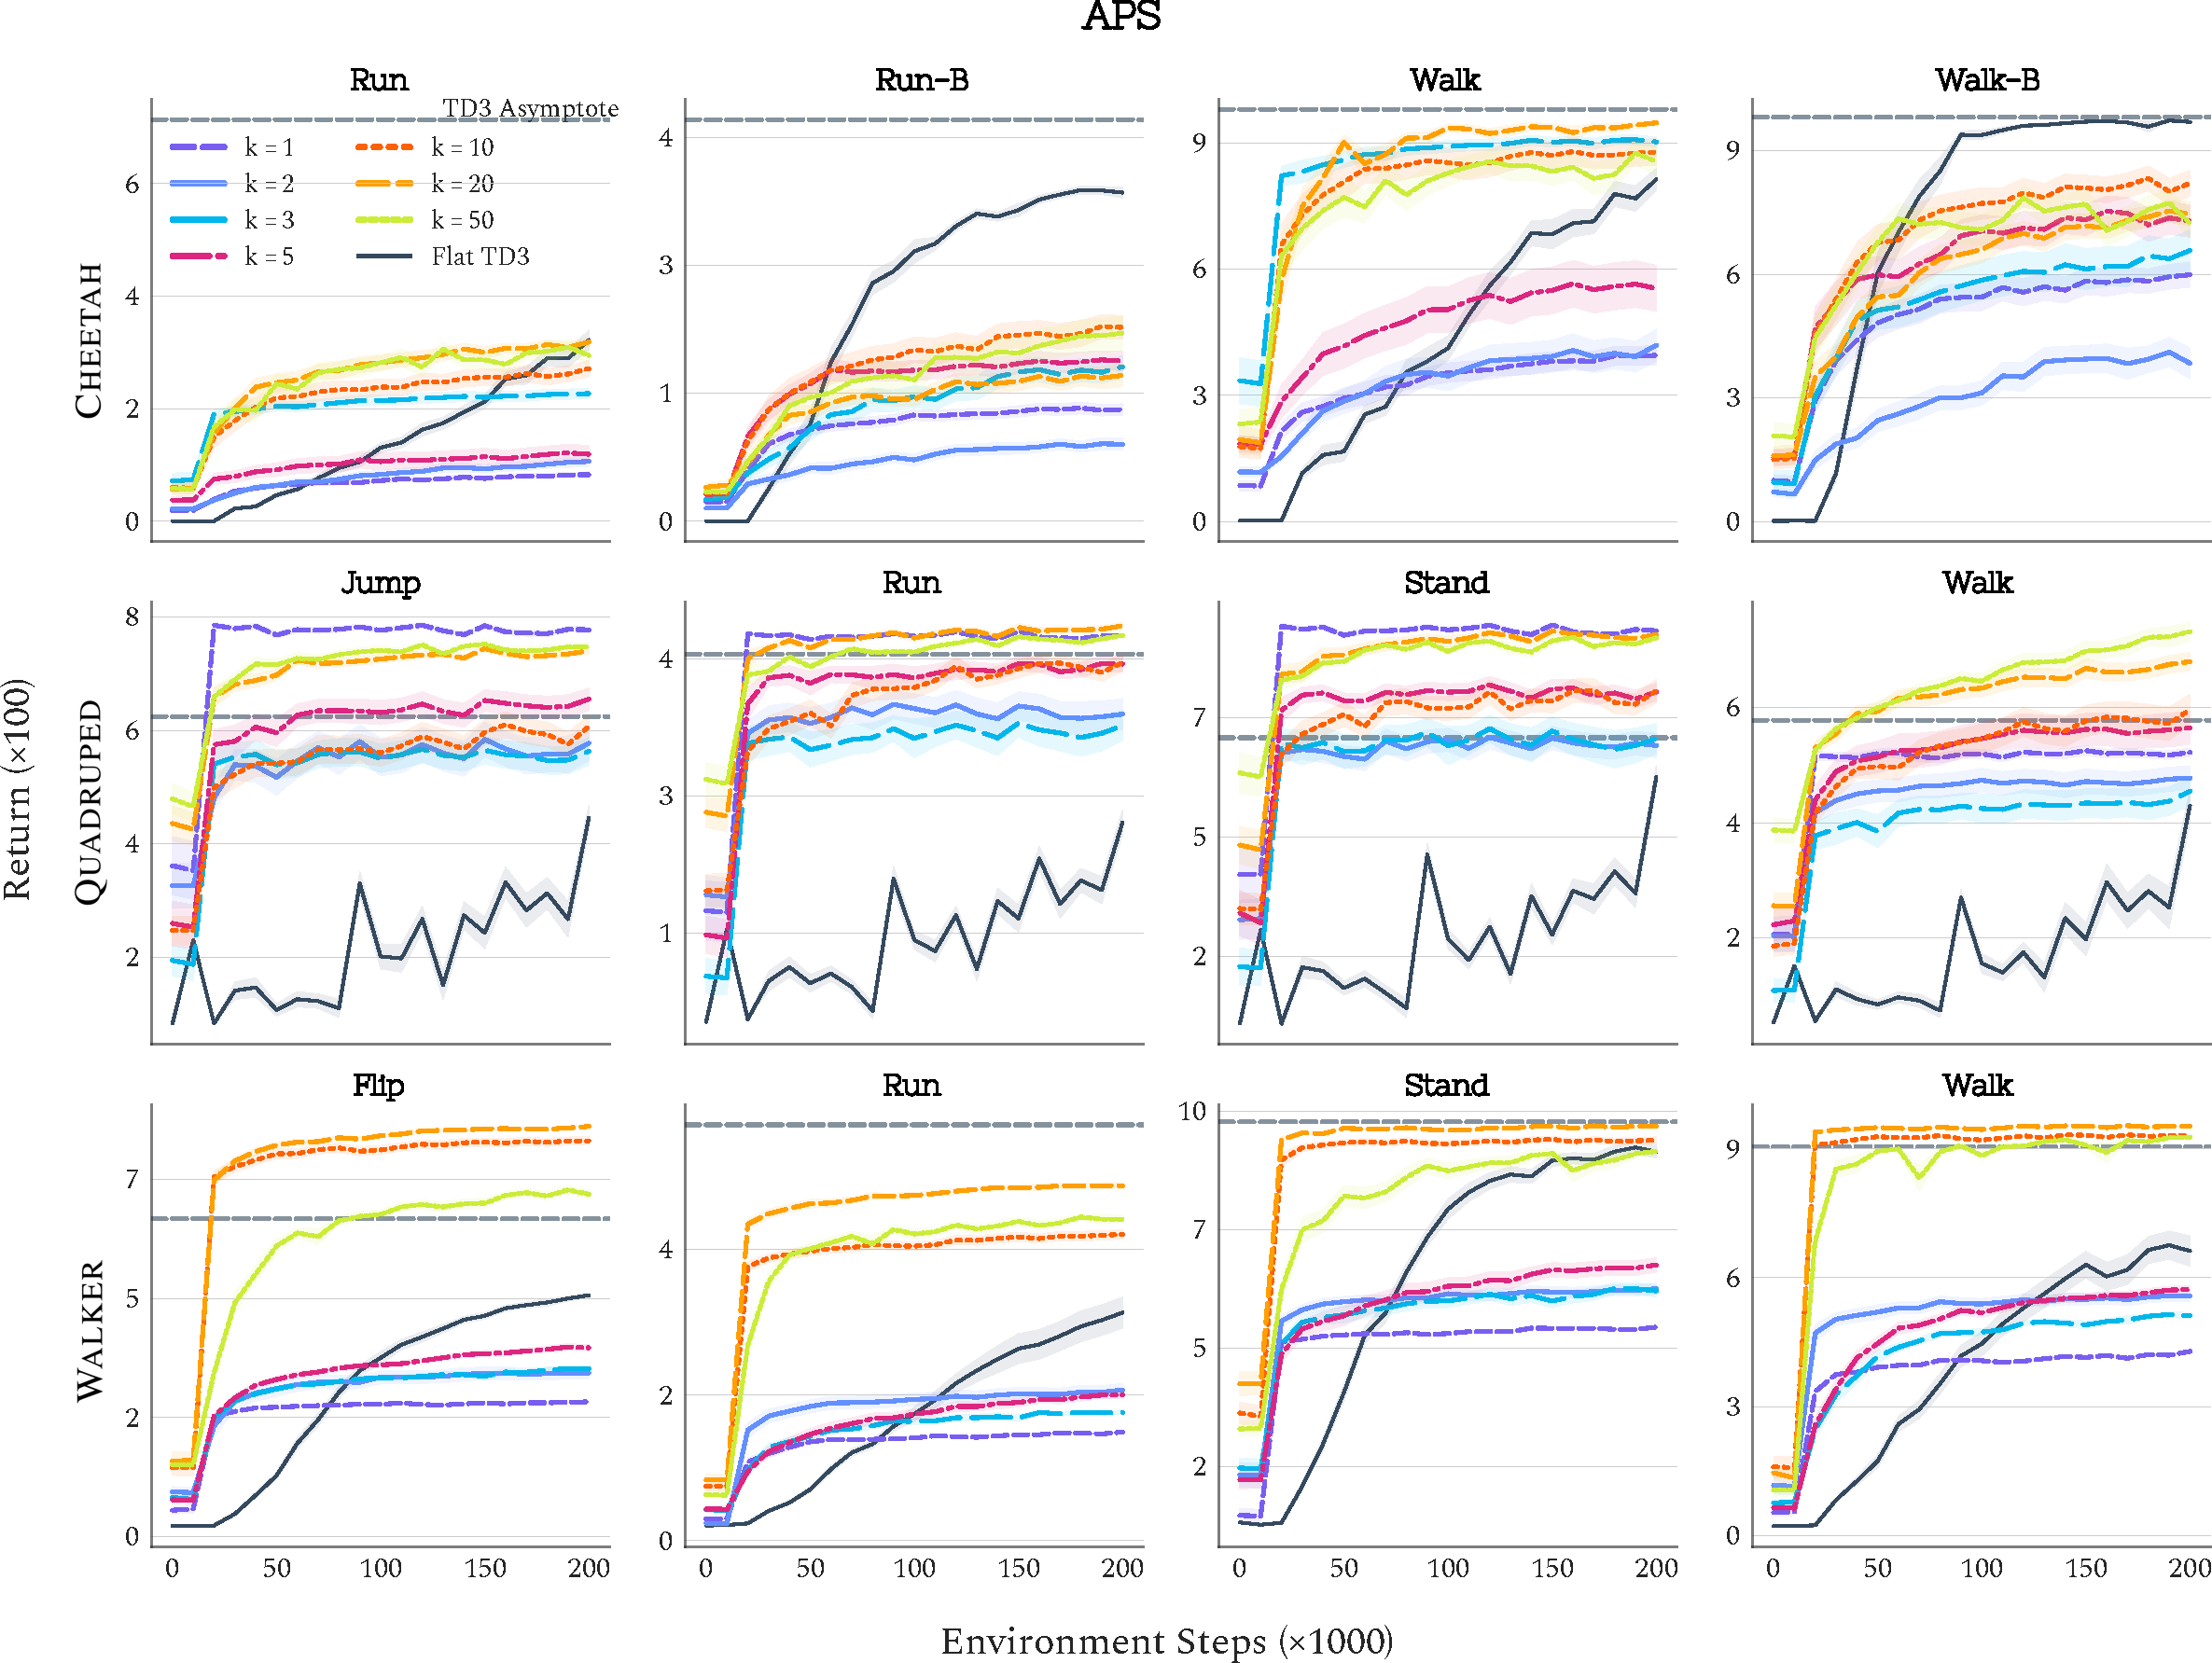
\includegraphics[width=.9\textwidth]{lk-curves-aps.pdf}}
\caption{Evaluation curves for LK pre-trained on the \texttt{APS} dataset with varying basis sizes, and for a flat TD3 agent. Shaded region indicates the standard error estimated over 30 independent runs.}
\label{fig:lk-curve-aps}
\end{figure*}



\begin{figure*}
\centerline{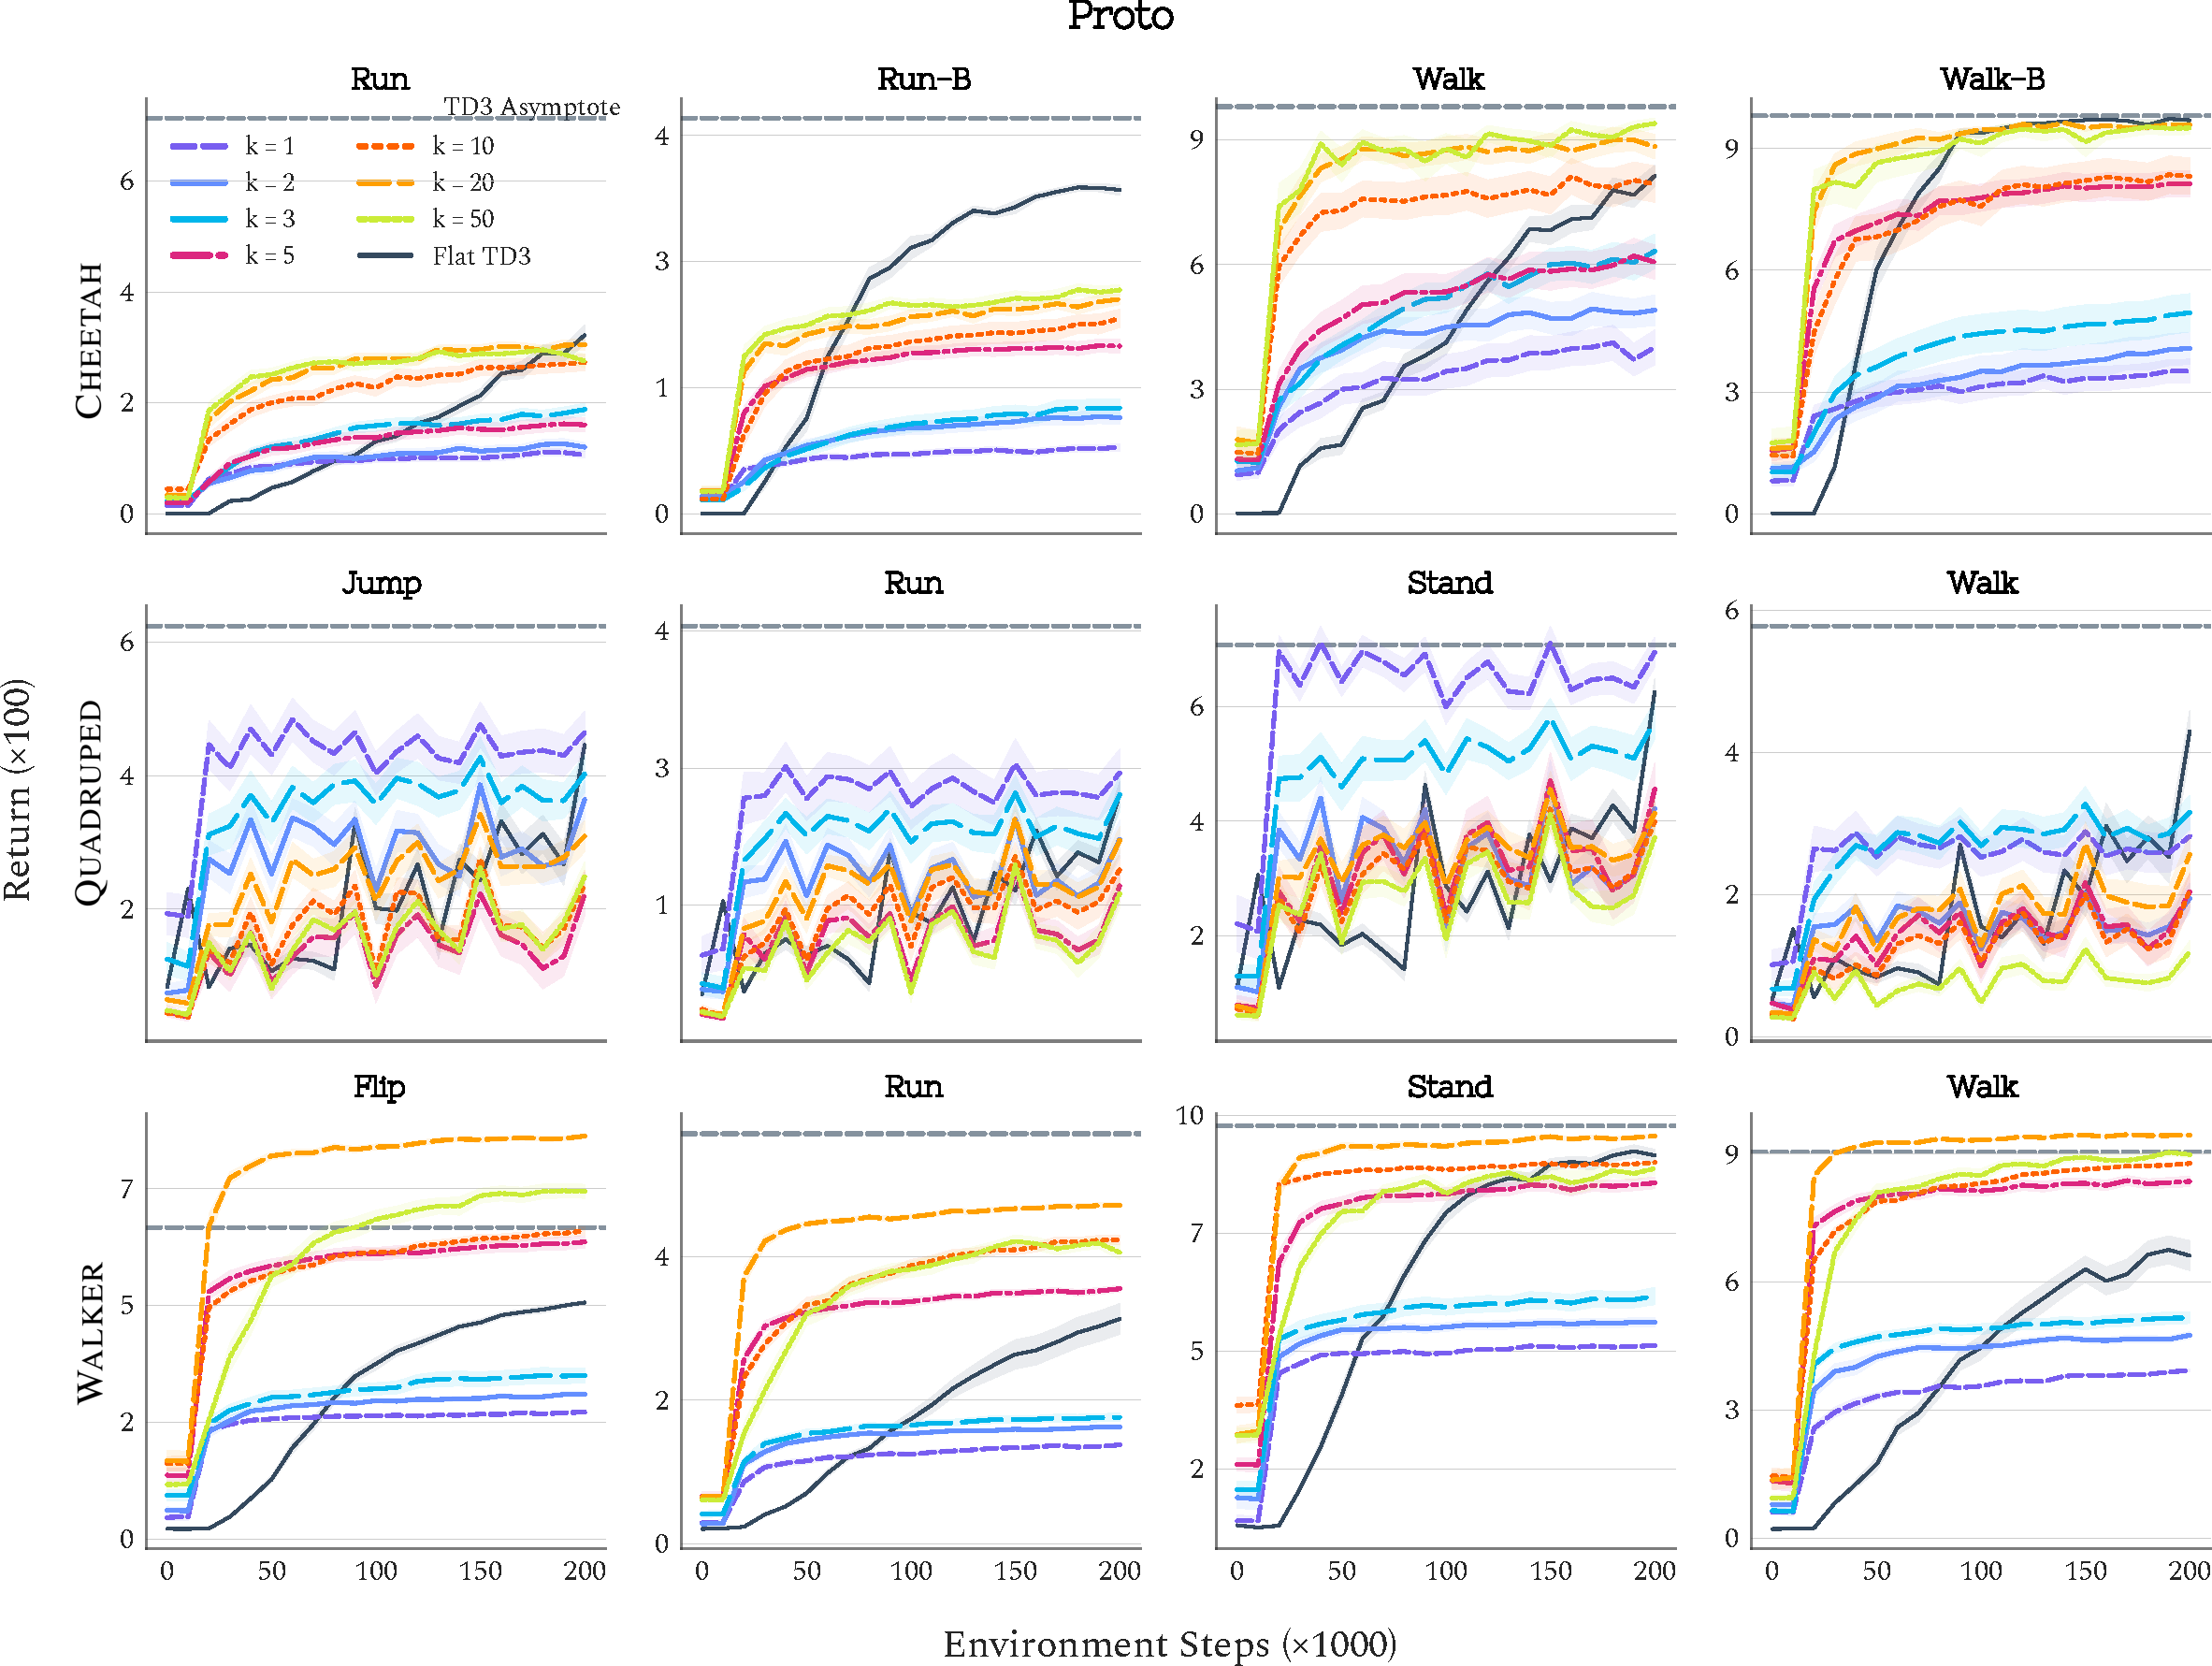
\includegraphics[width=.8\textwidth]{lk-curves-proto.pdf}}
\caption{Evaluation curves for LK pre-trained on the \texttt{Proto} dataset with varying basis sizes, and for a flat TD3 agent. Shaded region indicates the standard error estimated over 30 independent runs.}
\label{fig:lk-curve-proto}
\end{figure*}


\begin{figure*}
\centerline{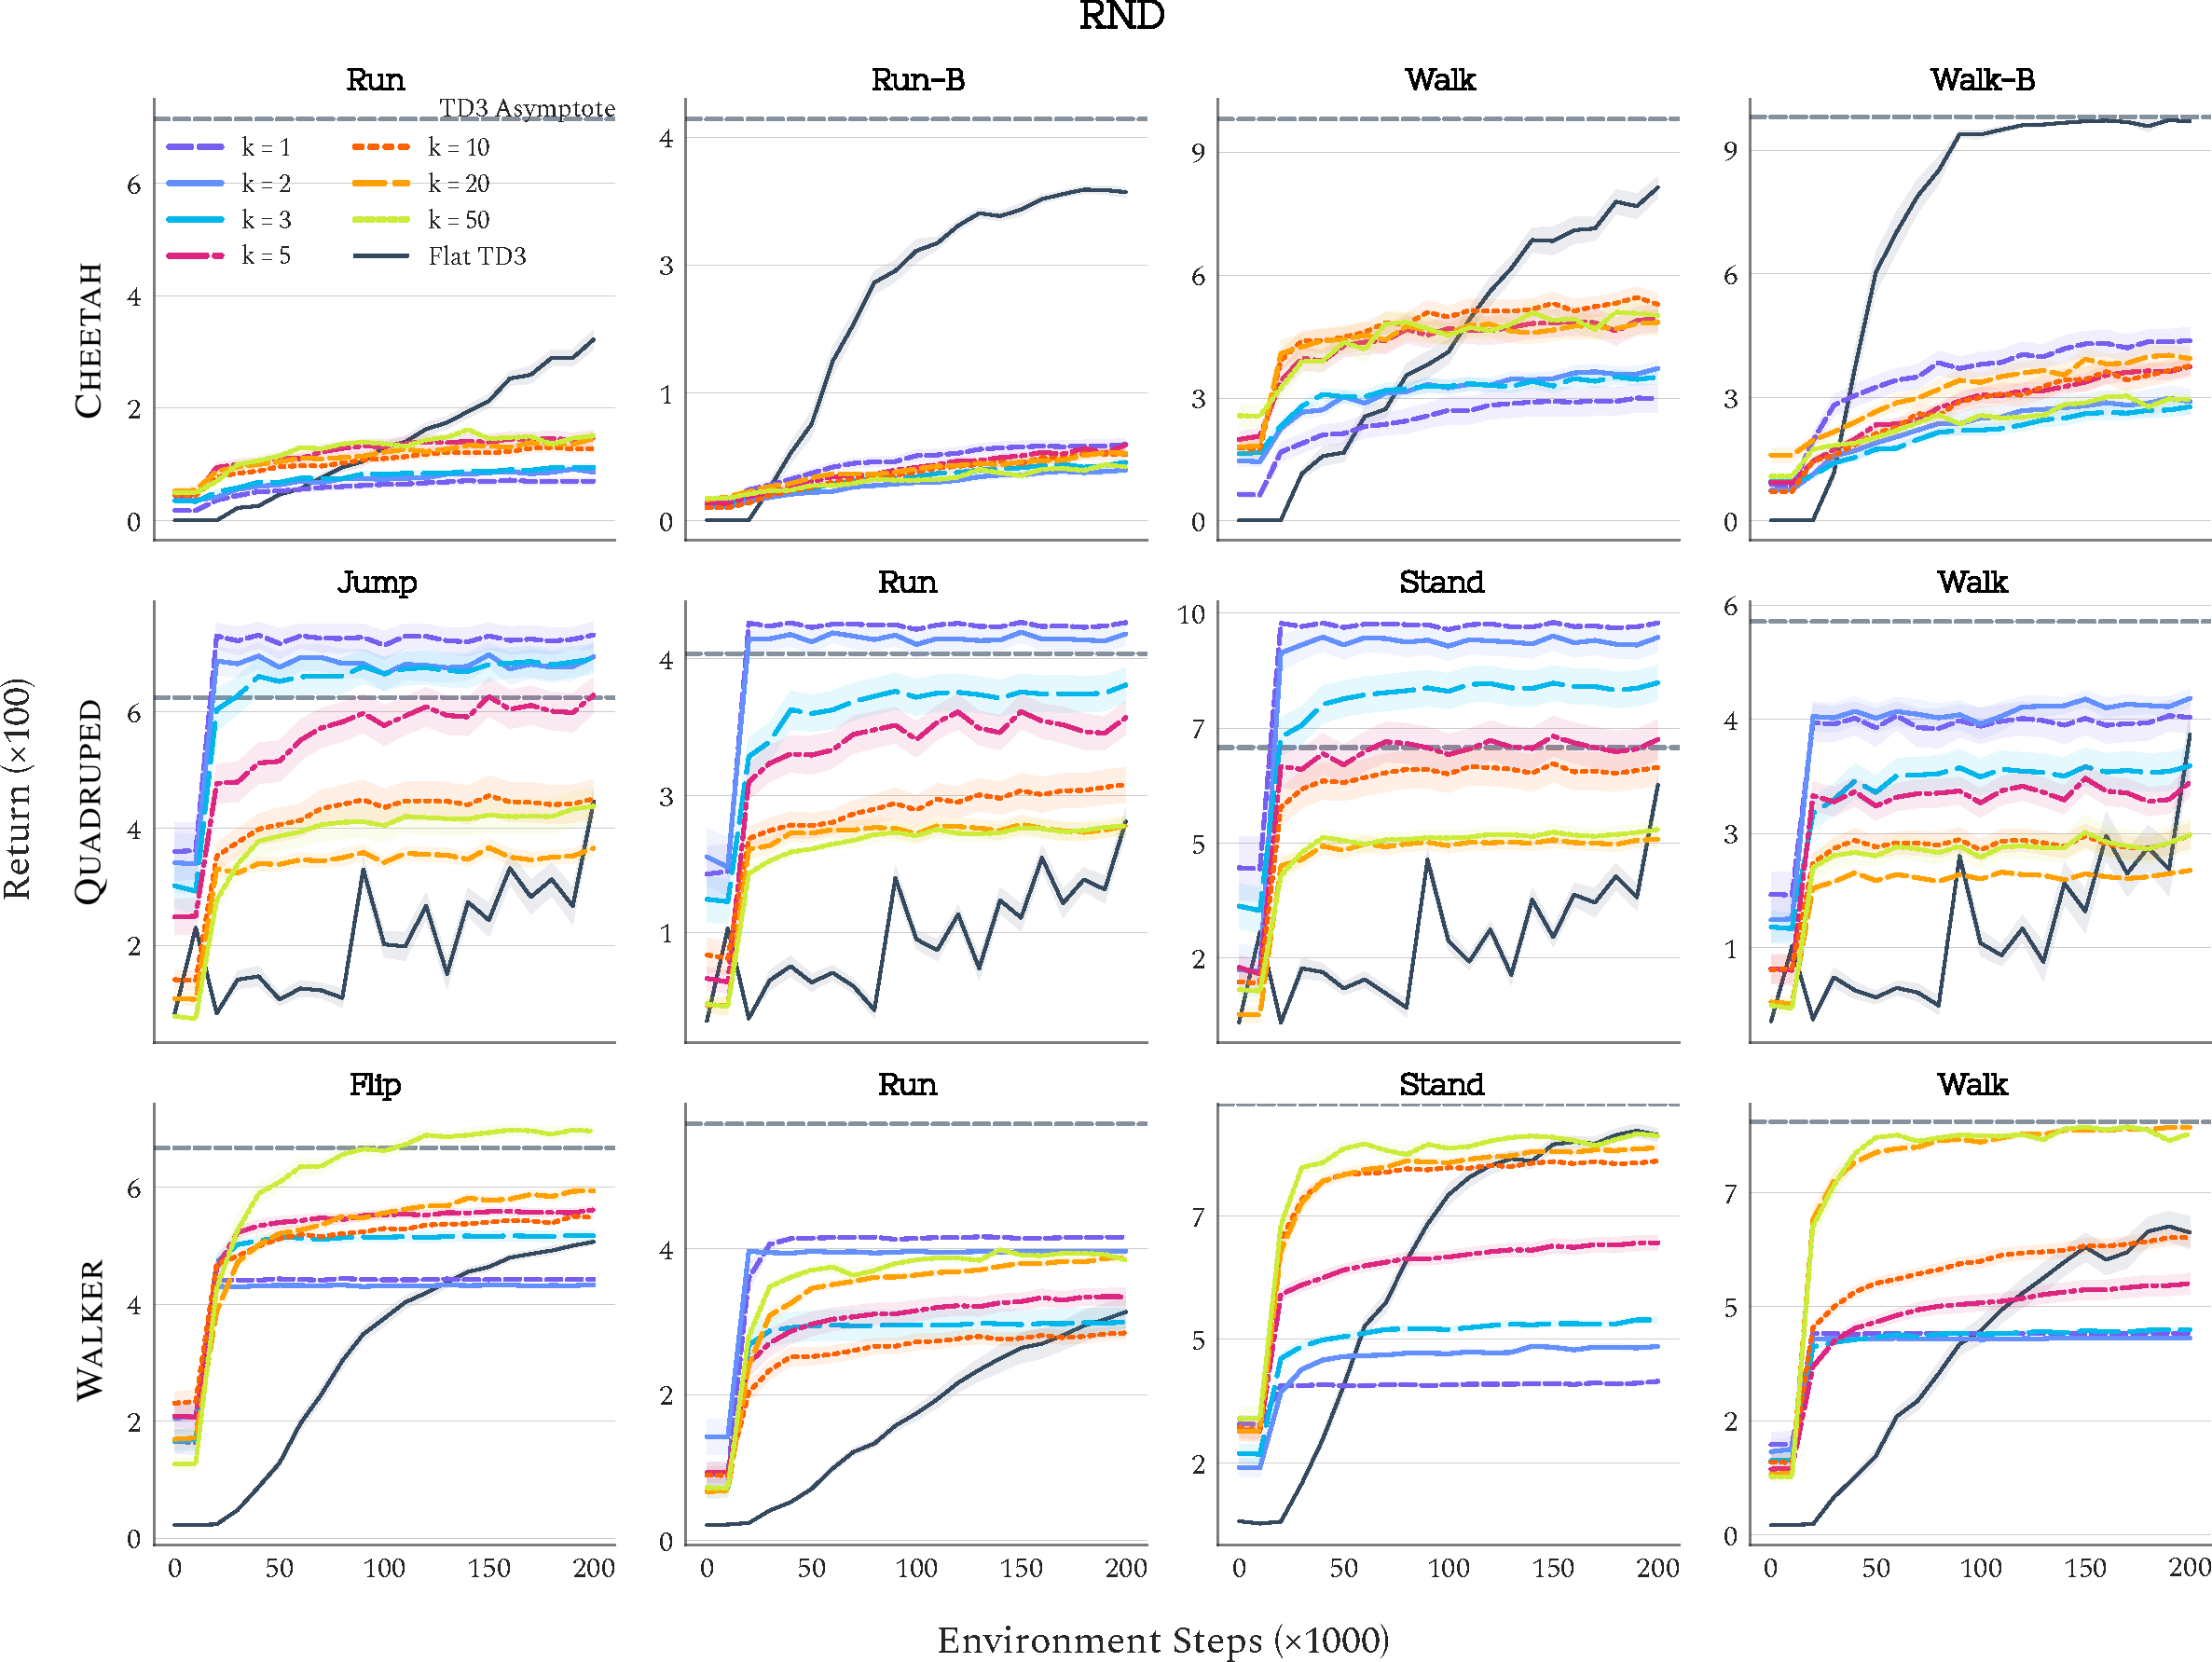
\includegraphics[width=.8\textwidth]{lk-curves-rnd.pdf}}
\caption{Evaluation curves for LK pre-trained on the \texttt{RND} dataset with varying basis sizes, and for a flat TD3 agent. Shaded region indicates the standard error estimated over 30 independent runs.}
\label{fig:lk-curve-rnd}
\end{figure*}


\newpage



% \begin{table}[H]
% \centering
% \caption{Relative percentage improvement of LK over its zero-shot baseline for varying basis sizes, averaged over 30 independent runs.}
% \label{tab:perc_imp_fb_lk_appendix}

% \setlength{\tabcolsep}{5pt}
% \footnotesize

% \begin{tabular}{
%   l
%   S[table-format=4.0] S[table-format=4.0]
%   S[table-format=4.0] S[table-format=4.0]
%   S[table-format=4.0] S[table-format=4.0]
%   S[table-format=4.0] S[table-format=4.0]
%   S[table-format=4.0] S[table-format=4.0]
%   S[table-format=3.0] S[table-format=3.0]
%   S[table-format=3.0] S[table-format=3.0]
% }
% \toprule
% & \multicolumn{14}{c}{\textbf{Zero-shot performance}} \\
% \cmidrule(lr){2-15}
% \textbf{Task}
% & \multicolumn{2}{c}{$k{=}1$}
% & \multicolumn{2}{c}{$k{=}2$}
% & \multicolumn{2}{c}{$k{=}3$}
% & \multicolumn{2}{c}{$k{=}5$}
% & \multicolumn{2}{c}{$k{=}10$}
% & \multicolumn{2}{c}{$k{=}20$}
% & \multicolumn{2}{c}{$k{=}50$} \\
% \cmidrule(lr){2-3}
% \cmidrule(lr){4-5}
% \cmidrule(lr){6-7}
% \cmidrule(lr){8-9}
% \cmidrule(lr){10-11}
% \cmidrule(lr){12-13}
% \cmidrule(lr){14-15}
% & FB & LK
% & FB & LK
% & FB & LK
% & FB & LK
% & FB & LK
% & FB & LK
% & FB & LK \\
% \midrule

% \rowcolor{gray!15} \domainavg{cheetah} & \multicolumn{14}{c}{} \\
% \hspace{.5em} \texttt{Run} & 16 & 10 & 36 & 6 & 90 & 66 & 106 & 92 & 175 & 147 & 254 & 184 & 248 & 196 \\
% \hspace{.5em} \texttt{Run-B} & 28 & 11 & 44 & 13 & 43 & 24 & 84 & 76 & 142 & 142 & 236 & 181 & 229 & 188 \\
% \hspace{.5em} \texttt{Walk} & 83 & 49 & 156 & 28 & 366 & 298 & 412 & 404 & 643 & 591 & 807 & 667 & 819 & 709 \\
% \hspace{.5em} \texttt{Walk-B} & 148 & 55 & 193 & 68 & 196 & 123 & 397 & 324 & 617 & 507 & 908 & 678 & 912 & 706 \\
% \addlinespace
% \rowcolor{gray!15} \domainavg{quadruped} & \multicolumn{14}{c}{} \\
% \hspace{.5em} \texttt{Jump} & 676 & 676 & 630 & 630 & 639 & 639 & 623 & 623 & 586 & 586 & 521 & 521 & 554 & 554 \\
% \hspace{.5em} \texttt{Run} & 433 & 433 & 411 & 411 & 411 & 411 & 422 & 422 & 375 & 375 & 334 & 334 & 366 & 366 \\
% \hspace{.5em} \texttt{Stand} & 862 & 862 & 824 & 824 & 830 & 830 & 831 & 831 & 746 & 746 & 672 & 672 & 705 & 705 \\
% \hspace{.5em} \texttt{Walk} & 447 & 447 & 413 & 413 & 412 & 412 & 424 & 424 & 376 & 376 & 376 & 376 & 410 & 410 \\
% \addlinespace
% \rowcolor{gray!15} \domainavg{walker} & \multicolumn{14}{c}{} \\
% \hspace{.5em} \texttt{Flip} & 60 & 161 & 397 & 182 & 384 & 201 & 314 & 259 & 351 & 253 & 419 & 518 & 412 & 507 \\
% \hspace{.5em} \texttt{Run} & 35 & 152 & 330 & 168 & 333 & 162 & 296 & 165 & 324 & 143 & 309 & 282 & 356 & 294 \\
% \hspace{.5em} \texttt{Stand} & 192 & 226 & 279 & 232 & 466 & 280 & 582 & 416 & 537 & 398 & 702 & 525 & 754 & 635 \\
% \hspace{.5em} \texttt{Walk} & 51 & 156 & 489 & 225 & 534 & 163 & 501 & 209 & 530 & 417 & 680 & 696 & 816 & 890 \\
% \addlinespace


% \bottomrule

% \end{tabular}
% \end{table}



\begin{figure*}[t]
\centerline{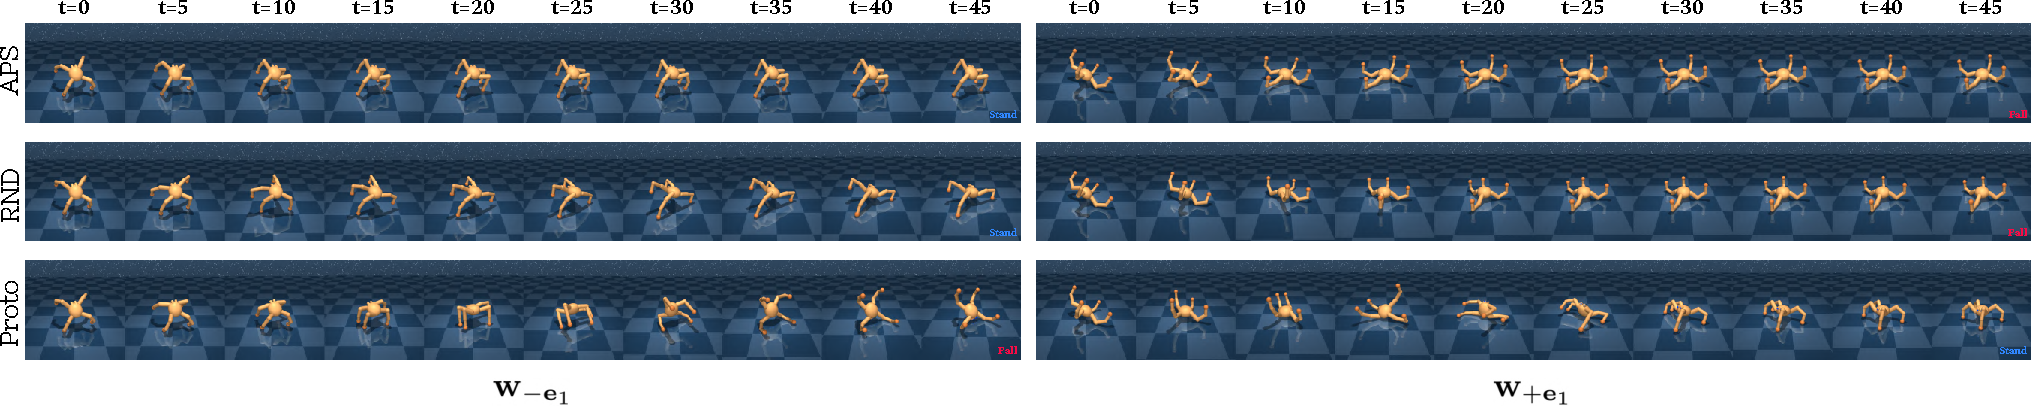
\includegraphics[width=\textwidth]{quadruped_behaviors_compressed.pdf}}
\caption{Behaviors induced by $\mathbf{w}_{\mathbf{-e_{1}}}$ and $\mathbf{w}_{\mathbf{+e_{1}}}$ in the \textsc{Quadruped} domain in all three dataset.}
\label{fig:quadruped-more}
\end{figure*}



\newpage 

\section{The Curious Case of \textsc{Quadruped}}
\label{sec:quadruped}

In this section, we analyze the behaviors induced by the weight vectors $\mathbf{w}_{-\mathbf{e}_1}$ and $\mathbf{w}_{+\mathbf{e}_1}$ in \textsc{Quadruped} to characterize their role in task performance. Across all three datasets and independent runs, these vectors consistently induce two dominant behaviors: maintaining an upright posture or collapsing onto the back (see Figure~\ref{fig:quadruped-more}). From arbitrary initial configurations, conditioning on $\mathbf{w}_{-\mathbf{e}_1}$ or $\mathbf{w}_{+\mathbf{e}_1}$ modulates the torso’s elevation relative to the ground, effectively controlling upright versus collapsed postures. \looseness=-1

Coincidentally, all four \textsc{Quadruped} tasks include an uprightness term that measures alignment between the torso’s vertical axis and the global vertical axis. The \texttt{Stand} task is defined solely by this term and encourages recovery from arbitrary initial orientations. The \texttt{Jump} task modulates the uprightness term with a height-dependent factor that increases with center-of-mass elevation and saturates at a target height. The \texttt{Walk} and \texttt{Run} tasks further scale the uprightness term by a forward-velocity factor that saturates at task-specific target speeds, with \texttt{Walk} favoring lower-speed locomotion and \texttt{Run} favoring higher-speed locomotion.

This shared uprightness structure aligns closely with the behaviors induced by $\mathbf{w}_{-\mathbf{e}_1}$ and $\mathbf{w}_{+\mathbf{e}_1}$, providing a direct explanation for the strong performance observed when using only the leading eigenvector as the basis. Figure~\ref{fig:quadruped-weight-trend} illustrates this effect by showing the estimated zero-shot weight vectors across tasks and basis sizes on the \texttt{APS} dataset. Across all conditions, the coefficient corresponding to the first basis component consistently dominates, indicating that it captures the primary reward-aligned direction. Additional eigenvectors contribute comparatively little and primarily introduce representational overhead, which correlates with the observed degradation in zero-shot performance as the basis size increases.

Consistent with this interpretation, Figure~\ref{fig:lk-lineplot-appendix} shows that average performance decreases as task rewards deviate from a pure uprightness objective, following the ordering \texttt{Stand} $>$ \texttt{Jump} $>$ \texttt{Walk} $\approx$ \texttt{Run}. Tasks that introduce additional height- or velocity-dependent modulation require structure beyond the dominant basis direction, reducing the effectiveness of a minimal representation.



\begin{figure*}
\centerline{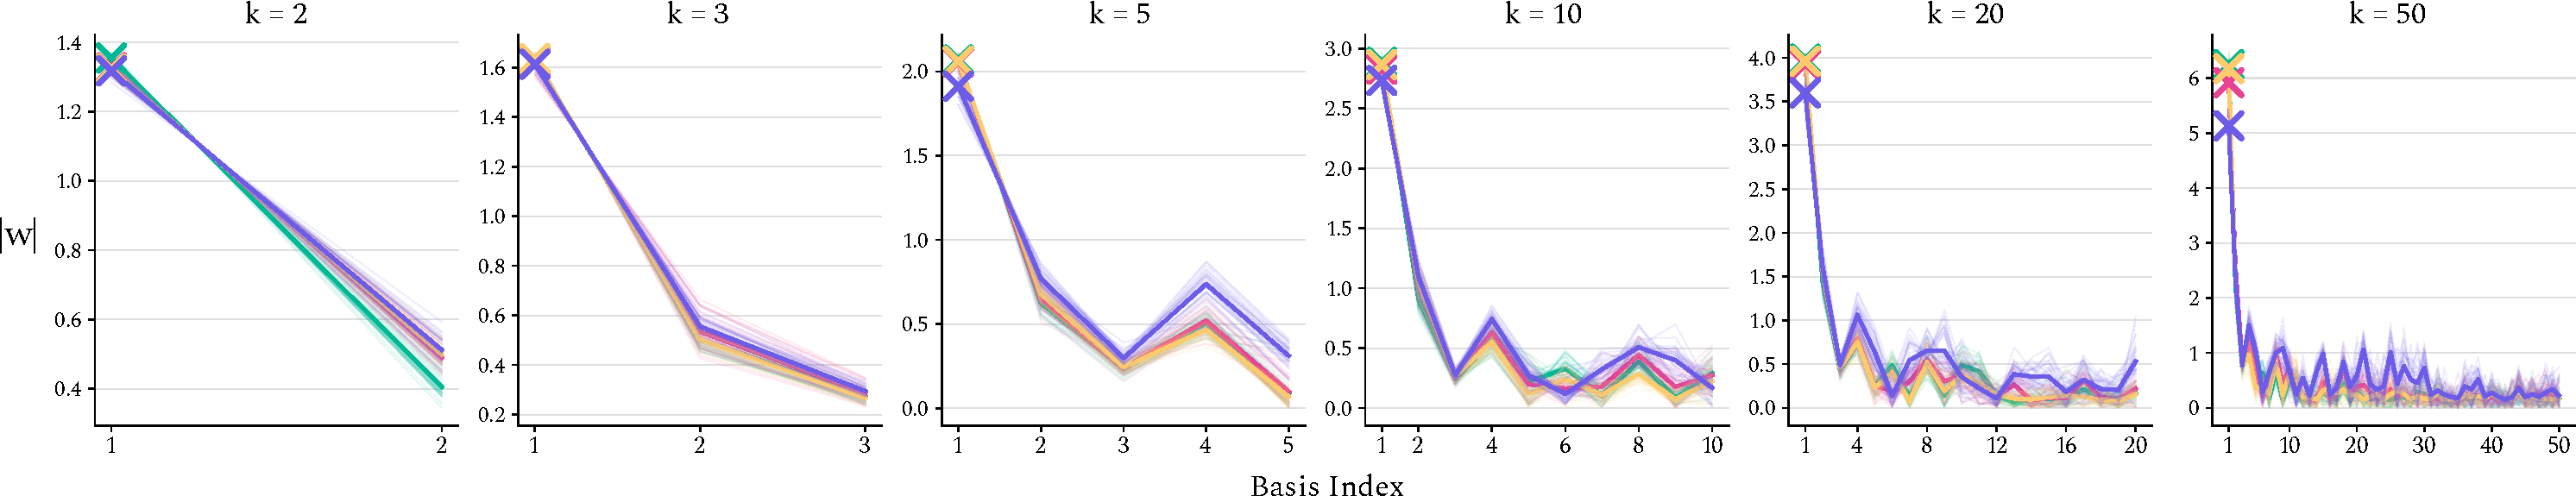
\includegraphics[width=\textwidth]{quadruped_weights.pdf}}
\caption{Absolute zero-shot weight magnitudes for all tasks, grouped by basis size. Each subplot shows all task-specific weights with low opacity, together with the mean absolute weight plotted as a thick line. Note that the entries in the $x$-axis are different indices for the weight magnitudes, there is no notion of time progression or size within a single panel; we connect the datapoints with a line to ease visualization. The first basis coefficient is indicated by a cross.}
\label{fig:quadruped-weight-trend}
\end{figure*}


\newpage

\section{Pseudocode for training Laplacian Keyboard}

We present Python-style pseudocode for training the Laplacian encoder and USFA during pre-training, and the meta-policy during downstream learning. Low-level implementation details are omitted for clarity.

\vspace{10pt}

\begin{lstlisting}[
    language=Python,
    basicstyle=\ttfamily\small,
    backgroundcolor=\color{codebg},
    commentstyle=\color{commentcolor}\itshape,
    keywordstyle=\color{keywordcolor}\bfseries,
    stringstyle=\color{stringcolor},
    numbers=left,
    numberstyle=\tiny\color{commentcolor},
    numbersep=8pt,
    frame=single,
    framexleftmargin=15pt,
    xleftmargin=40pt,
    linewidth=0.85\textwidth,
    tabsize=4,
    breaklines=true,
    showstringspaces=false,
    morekeywords={self, def, return}
]
def train_laplacian_encoder(self):

    # sample contrastive state pairs
    obs, pos_obs, neg_obs = self.sample_laplacian_batch()

    # encode states
    phi      = self.encoder(obs)
    phi_pos  = self.encoder(pos_obs)
    phi_neg  = self.encoder(neg_obs)

    # graph-smoothness loss
    graph_loss = ((phi - phi_pos) ** 2).mean()

    # orthogonality-enforcing loss
    error = compute_orthogonality_error(phi, phi_neg)

    dual_loss    = (self.dual_vars.detach() * error).sum()
    barrier_loss = (self.barrier_coefs.detach() * error.pow(2)).sum()

    # optimize encoder
    loss = graph_loss + dual_loss + barrier_loss
    self.encoder_optimizer.step()
\end{lstlisting}

\vspace{10pt}


\begin{lstlisting}[
    language=Python,
    basicstyle=\ttfamily\small,
    backgroundcolor=\color{codebg},
    commentstyle=\color{commentcolor}\itshape,
    keywordstyle=\color{keywordcolor}\bfseries,
    stringstyle=\color{stringcolor},
    numbers=left,
    numberstyle=\tiny\color{commentcolor},
    numbersep=8pt,
    frame=single,
    framexleftmargin=15pt,
    xleftmargin=40pt,
    linewidth=0.85\textwidth,
    tabsize=4,
    breaklines=true,
    showstringspaces=false,
    morekeywords={self, def, return}
]
def train_usfa(self):

    # sample transition batch
    obs, action, next_obs, done = self.sample_usfa_batch()
    w = self.sample_task_weight()

    # compute Laplacian features
    phi      = self.encoder(obs)
    phi_next = self.encoder(next_obs)

    # sample next action
    next_action = self.actor(phi_next, w).sample()

    # compute target successor features
    psi_target = phi + (1 - done) * self.gamma * \
        self.target_psi(phi_next, next_action, w)

    # predict successor features
    psi_pred = self.psi(phi, action, w)

    # TD loss
    psi_loss = mse(psi_pred - psi_target.detach())
    self.psi_optimizer.step()

    # optionally update actor
    if update_actor:
        actor_loss = -(psi_pred * w).sum(-1).mean()
        self.actor_optimizer.step()

    # update target networks
    self.update_target_networks()
\end{lstlisting}


\newpage

\begin{lstlisting}[
    language=Python,
    basicstyle=\ttfamily\small,
    backgroundcolor=\color{codebg},
    commentstyle=\color{commentcolor}\itshape,
    keywordstyle=\color{keywordcolor}\bfseries,
    stringstyle=\color{stringcolor},
    numbers=left,
    numberstyle=\tiny\color{commentcolor},
    numbersep=8pt,
    frame=single,
    framexleftmargin=15pt,
    xleftmargin=40pt,
    linewidth=0.85\textwidth,
    tabsize=4,
    breaklines=true,
    showstringspaces=false,
    morekeywords={self, def, return}
]
def train_downstream(self):
    obs = self.env.reset()
    done = False
    option_return = 0
    option_length = 0

    # sample initial option
    w = self.meta_actor(obs)

    while not done:

        # act using USFA-conditioned policy
        action = self.actor(obs, w).sample()
        next_obs, reward, done = self.env.step(action)

        # accumulate option return
        option_return += (self.gamma ** option_length) * reward
        option_length += 1

        # terminate option
        if option_length >= self.max_option_length or done:
            self.replay_buffer.store(obs, w, next_obs,
                                     option_return, done)
            w = self.meta_actor(next_obs)
            option_return = 0
            option_length = 0

        obs = next_obs

        # update meta-policy
        if update_meta:
            batch = self.replay_buffer.sample()
            self.update_critic(batch)
            self.update_actor(batch)
            self.update_target_networks()
\end{lstlisting}


\end{document}
